% ============================================================
% IPDC Digital OSS Thesis - Main Document
% Nankai University, College of Software
% Kebede Yetnayet Berhanu - December 2025
%
% Based on NKU_thesis_graduate-2024 official template
% Compile with: XeLaTeX [recommended] or PDFLaTeX
% ============================================================
\documentclass[12pt,openany]{book}

% --- Mathematics ---
\usepackage{amsmath,amssymb}
\usepackage{pifont}

% --- Hyperlinks ---
\usepackage[unicode,bookmarksnumbered]{hyperref}

% --- NKThesis Package (English mode) ---
\usepackage[emptydoublepage,English]{NKThesis}

% --- Bibliography (biblatex with NKThesis style, natbib compatibility) ---
\usepackage[backend=bibtex8, defernumbers=true, sorting=nty, style=nkthesis, natbib=true]{biblatex}
\addbibresource{references.bib}
\DeclareBibliographyCategory{cited}
\AtEveryCitekey{\addtocategory{cited}{\thefield{entrykey}}}

% --- Hyperlink Colors ---
\hypersetup{colorlinks=true,
            pdfborder=0 0 1,
            citecolor=black,
            linkcolor=black}

% --- Graphics and Figures ---
\usepackage{tikz}
\usetikzlibrary{shapes.geometric, arrows.meta, positioning, fit, calc}
\usepackage{float}
\graphicspath{{figures/}}

% --- Tables ---
\usepackage{booktabs}
\usepackage{longtable}
\usepackage{array}
\usepackage{multirow}
\usepackage{tabularx}

% --- Code Listings ---
\usepackage{listings}
\lstset{
  basicstyle=\ttfamily\small,
  breaklines=true,
  frame=single,
  numbers=left,
  numberstyle=\tiny,
  tabsize=2
}

% --- Misc ---
\usepackage{xcolor}
\usepackage{pdfpages}

% --- Allow line breaks in monospace text ---
\usepackage[htt]{hyphenat}

% --- Custom Commands ---
\newcommand{\tbf}[1]{\textbf{#1}}

% ============================================================
\begin{document}
\raggedbottom
\sloppy

% --- Thesis Metadata (auto-generates: Cover + Declaration + Authorization) ---
\NKTsetup{%
  论文题目(中文) = 面向埃塞俄比亚工业园区发展公司的离线优先数字一站式服务平台,
  副标题        = ——将中国智慧园区模式本地化应用于网络受限环境,
  论文题目(英文) = {Offline-First Digital One-Stop-Shop for Ethiopian
  Industrial Parks Development Corporation (IPDC):
  Localizing China Smart Park Model for
  Connectivity-Constrained Environments},
  论文作者       = Kebede Yetnayet Berhanu,
  学号           = 2120246030,
  指导教师       = 张海宁,
  指导教师职称   = 教授,
  申请学位       = 工学硕士,
  培养单位       = 软件学院,
  学科专业       = 软件工程,
  研究方向       = 数字平台开发,
  答辩委员会主席  = ,
  评阅人       = ,
  中图分类号     = TP311,
  UDC            = ,
  学校代码       = 10055,
  密级           = 公开,
  保密期限       = ,
  审批表编号     = ,
  批准日期       = ,
  论文完成时间   = 二〇二五年十二月,
  答辩日期       = ,
  签字日期       = 2025\quad 年\quad 12 \quad 月\quad \quad 日,
  论文类别       = 学历硕士,
  院/系/所       = 软件学院,
  专业           = 软件工程,
  联系电话       = ,
  Email          = ,
  通讯地址(邮编) = 天津经济开发区宏达街23号南开大学泰达校区（300457）,
  备注           =
}

% --- Abstract (Chinese + English) ---
% ============================================================
% Abstracts - Chinese (摘要) + English (Abstract)
% Using NKThesis custom environments
% ============================================================

% --- Chinese Abstract (摘要) ---
\begin{zhaiyao}

埃塞俄比亚工业园区发展公司（IPDC）管辖的多个工业园区目前仍依赖纸质行政流程，导致服务交付延迟、费用收缴效率低下，并引发利益相关方的不满。在中国，基于企业微信和钉钉构建的智慧园区平台已在数字化治理方面取得显著成效，但这些平台依赖稳定的互联网连接——而埃塞俄比亚工业园区无法保证这一条件，日均网络中断时间长达三至五小时。

本研究旨在为IPDC设计、开发并评估一个离线优先的数字一站式服务平台，以渐进式网络应用程序（PWA）形式交付。研究采用设计科学研究方法论，将中国智慧园区模式适配到网络受限环境中。三个研究问题贯穿全文：（1）如何系统地将中国数字治理模式迁移到非洲环境；（2）如何架构一个支持复杂工业工作流的离线优先PWA；（3）在服务多个利益相关方群体的平台中，应以何种设计原则指导功能优先级决策。

所开发的原型系统支持离线服务请求提交并在网络恢复后自动同步，提供基于角色的差异化界面，以及用于跟踪服务费用的数字令牌系统。由于采用PWA技术构建，该平台可通过单一代码库在桌面端和移动端浏览器上运行，无需开发独立的原生移动应用。Firebase Firestore作为后端服务，提供内置的离线数据持久化能力。系统还集成了三个机器学习模型：自动服务分类模型、预测性设备维护模型以及面向潜在租户的工业园区推荐模型。

本研究做出四项贡献：（1）提出技术适配框架，指导数字治理模式在不同网络条件下的跨境迁移；（2）设计离线优先工业服务架构，扩展PWA能力以支持复杂工作流；（3）建立一套设计原则，用于确定离线使用场景下的功能优先级；（4）开发首个面向埃塞俄比亚工业园区的专用数字平台。这些成果为非洲及其他发展中地区在网络受限环境下的数字化转型提供了可复制的方法。

\end{zhaiyao}

\begin{guanjianci}
离线优先架构，渐进式网络应用，数字一站式服务，智慧工业园区，设计科学研究，技术适配，埃塞俄比亚工业园区
\end{guanjianci}


% --- English Abstract ---
\begin{abstract}

Several industrial parks managed by the Ethiopian Industrial Parks Development Corporation (IPDC) still rely on paper-based administrative processes, resulting in delayed service delivery, inefficient fee collection, and mounting frustration among stakeholders. In China, smart park platforms built on WeChat Work and DingTalk have demonstrated real effectiveness for digital governance --- yet they depend on stable internet connectivity that Ethiopian parks cannot guarantee, where daily outages routinely last three to five hours.

An offline-first digital one-stop service for IPDC --- delivered as a Progressive Web Application (PWA) --- is both the research output and the vehicle for answering these questions. Drawing on Design Science Research methodology, the study adapts Chinese smart park models for environments with limited connectivity. Three research questions guide the work: (1) how to systematically transfer Chinese digital governance models to African settings; (2) how to architect an offline-first PWA that handles complex industrial workflows; and (3) what design principles should govern feature prioritization in platforms serving multiple stakeholder groups.

The resulting prototype supports offline service request submission with automatic synchronization once connectivity returns, role-based interfaces for different stakeholders, and a digital token system for tracking service fees. Built as a PWA, the platform runs on both desktop and mobile browsers from a single codebase, eliminating the need for separate native mobile applications. Firebase Firestore serves as the backend, providing built-in offline data persistence. Three machine learning models are also integrated: one for automated service classification, one for predictive equipment maintenance, and one for recommending suitable industrial parks to prospective tenants.

Four contributions come out of this work. The Technology Adaptation Framework gives practitioners a structured way to transfer digital governance models across contexts with different connectivity constraints. The Offline-First Industrial Service Architecture shows how PWA capabilities can stretch to cover complex multi-stakeholder workflows. A set of Design Principles offers practical guidance on which features to prioritize for offline availability. And the platform itself is the first purpose-built digital one-stop service for Ethiopian industrial parks. Whether these lessons travel cleanly to other developing country contexts remains open --- but the offline-first approach demonstrated here gives organizations facing the same infrastructure gap somewhere concrete to start.

\end{abstract}

\begin{keywords}
Offline-First Architecture, Progressive Web Application, Digital One-Stop Service, Smart Industrial Park, Design Science Research, Technology Adaptation, Ethiopian Industrial Parks
\end{keywords}


% --- Table of Contents ---
\tableofcontents

% --- List of Figures ---
\listoffigures

% --- List of Tables ---
\listoftables

% --- Abbreviations ---
\chapter*{List of Abbreviations}
\markboth{List of Abbreviations}{List of Abbreviations}

\vspace{-0.5em}
{\small
\begin{tabular}{@{}ll@{}}
\toprule
\textbf{Abbreviation} & \textbf{Full Form} \\
\midrule
API & Application Programming Interface \\
BaaS & Backend as a Service \\
BRI & Belt and Road Initiative \\
CBE & Commercial Bank of Ethiopia \\
CORS & Cross-Origin Resource Sharing \\
CRDT & Conflict-free Replicated Data Type \\
CSS & Cascading Style Sheets \\
DSR & Design Science Research \\
DSRM & Design Science Research Methodology \\
ETB & Ethiopian Birr \\
HTML & HyperText Markup Language \\
ICT & Information and Communication Technology \\
ICT4D & ICT for Development \\
IPDC & Industrial Parks Development Corporation \\
JS & JavaScript \\
MoSCoW & Must Have, Should Have, Could Have, Won't Have \\
MUI & Material-UI \\
NoSQL & Not Only SQL \\
OSS & One-Stop-Shop \\
PIM & Park Innovation Management \\
PWA & Progressive Web Application \\
RBAC & Role-Based Access Control \\
SDK & Software Development Kit \\
SEZ & Special Economic Zone \\
SNNPR & Southern Nations, Nationalities, and Peoples' Region \\
SQL & Structured Query Language \\
SUS & System Usability Scale \\
UAT & User Acceptance Testing \\
UI & User Interface \\
UX & User Experience \\
WCAG & Web Content Accessibility Guidelines \\
\bottomrule
\end{tabular}}


% --- Main Chapters ---
\chapter{Introduction}
\label{ch:introduction}

\section{Background of the Study}

\subsection{Global Context: Digital Transformation in Industrial Parks}

Across the world, industrial parks have moved well beyond providing land and utilities. Smart technologies now sit at the centre of park strategy --- not just to cut administrative costs, but because tenants increasingly expect the same digital governance they encounter elsewhere. Integrated platforms that consolidate services, enable real-time communication, and generate operational data have become the benchmark \citep{Yang2025, Huang2023}.

China has gone further than most. Parks built around WeChat Work and DingTalk have changed how tenants and administrators interact: business registration, permit processing, facility management, and communication all flow through a single digital interface \citep{Huang2023, Schreieck2022}. That kind of integration is no longer a novelty --- it is a working demonstration of what digital park governance actually looks like.

The appeal of these models to other countries is obvious, particularly in developing economies whose industrial zones still run on manual administration. The Belt and Road Initiative (BRI) and its digital extension, the Digital Silk Road (DSR), have built practical pathways for technology exchange between China and partner countries across Africa \citep{LiuBRI2023, deKluiver2024, ElKadi2024}.

\subsection{Ethiopian Context: Industrial Parks and Digital Transformation}

Industrial park development sits at the centre of Ethiopia's economic strategy --- and the Industrial Parks Development Corporation (IPDC), established in 2014, is the institution charged with making it work \citep{Oqubay2015, IPDC2020}. Bole Lemi, Eastern Industrial Zone, Hawassa, and a growing number of other parks host domestic and international manufacturers whose exports and employment figures are central to the country's development plans \citep{Guteta2024, Tesfaw2023}.

China's involvement in Ethiopian industrial parks goes well beyond trade. Several parks were built with Chinese capital and technical expertise, and Chinese firms remain a substantial share of the tenant base. That relationship, already deep on the investment side, makes a natural case for examining whether the digital governance tools Chinese parks have developed could be adapted to serve Ethiopian ones \citep{Negesa2022}.

Where those tools are absent, the gap shows. Service requests still require in-person office visits. Approval processes give tenants little sense of where things stand. Fee collection means cash or a separate bank visit, with no system linking payments to the requests they cover. These are not small inefficiencies --- they create delays and frustration that shape how tenants experience IPDC and how they assess whether to stay or expand \citep{Guteta2022, Guteta2023}.

\subsection{The Connectivity Challenge: Infrastructure Constraints}

Building a digital platform for Ethiopian industrial parks runs straight into a stubborn infrastructure problem: internet connectivity is unreliable. Survey data and published statistics point to the same picture --- parks typically lose internet for three to five hours a day, with complete outages two to three times a month \citep{Ethiotelecom2023, ITU2023}. Chinese parks operate on stable high-speed networks; Ethiopian parks do not.

Infrastructure investment is underway \citep{WorldBank2022}, but the near term looks much the same as today. A platform that depends on a live server connection goes dark during every outage --- potentially more disruptive than the paper systems it was meant to replace, since at least paper works without a fibre link.

Chinese platforms like WeChat Work and DingTalk were built for persistent connectivity. Deploying them in Ethiopia without fundamental reworking would produce a system that fails exactly when it is most needed, and users would reasonably revert to manual processes. The adaptation challenge is not cosmetic --- it goes to the architecture itself.

\subsection{The Offline-First Paradigm: A Solution Framework}

The offline-first paradigm inverts the usual assumption: instead of treating connectivity as the default and failure as the exception, the application treats local operation as the baseline and the network as an optional enhancement. \citet{Kleppmann2019} put this plainly in their work on local-first software --- the application works fully without a network connection; connectivity, when it arrives, is used for synchronization.

Progressive Web Applications (PWAs) make this practical for web platforms. Service workers intercept network requests and serve cached responses when the network is absent; IndexedDB persists structured data locally; background synchronization pushes queued operations to the server once connectivity returns \citep{AterPWA2017, Majchrzak2018, Tandel2018}. Research confirms that PWAs match native apps on most user-facing criteria while offering a cross-platform reach that native development cannot: one codebase serves desktop browsers, mobile browsers, and installs on phones as an app-like experience \citep{AhnAllen2020, BiornHansen2017}.

Google's Firebase reinforces this architecture. Firestore's built-in offline persistence caches data automatically and synchronizes it when the network returns, without requiring the application to manage that transition explicitly \citep{GoogleFirebase2024}. The free tier --- 50,000 daily reads, 20,000 writes, 1~GB storage --- covers both prototype development and a pilot deployment. Taken together, Chinese smart park design thinking, offline-first PWA architecture, and Firebase's persistence layer form the basis for digital governance that does not depend on a reliable connection to remain useful.

\section{Statement of the Problem}

IPDC operates multiple industrial parks serving domestic and international manufacturers. These parks depend on efficient service systems to support tenant operations — business licensing, facility management, utility services, maintenance coordination, and regulatory compliance. The quality of these services directly affects tenant satisfaction, operational efficiency, and the broader success of Ethiopia's industrial park programme.

Currently, IPDC relies almost entirely on paper-based systems and disconnected communication channels. Tenants visit administrative offices in person to file service requests, track progress through informal follow-ups, and navigate opaque bureaucratic processes. Several interconnected problems follow from this:

\textbf{Service Delivery Inefficiency:} Paper workflows slow request processing and approval routing. Requests get lost, misdirected, or stalled when staff are unavailable. Without automated tracking, neither staff nor tenants can reliably tell where any request stands.

\textbf{Fee Collection Challenges:} Fee collection is fragmented and lacks transparency. Cash payments raise security concerns; bank transfers require separate branch visits; and reconciling payments with services is a manual, error-prone process with no integrated system linking requests to payment status.

\textbf{Communication Gaps:} Information flows through multiple informal channels between management, administrative staff, operations teams, and tenants. Important announcements may not reach everyone, and there is no structured mechanism for tenant feedback.

\textbf{Operational Opacity:} Without digital records, management cannot answer basic operational questions: How long does a typical request take to resolve? Which service categories generate the most complaints? Where are staffing bottlenecks occurring? These questions are fundamental to running a well-managed park, yet there is currently no systematic way to answer them.

\textbf{Stakeholder Frustration:} Ethiopian industrial parks compete for international investment. Tenant firms arriving from China, India, or other countries where park administration is already digital encounter a jarring step backward at IPDC. That experience shapes retention decisions and the attractiveness of IPDC parks to prospective investors who can compare alternatives.

Digitisation is the obvious answer, but conventional cloud-based platforms are a poor fit given the infrastructure constraints described above. Frequent outages would make cloud-dependent systems unavailable precisely when they are most needed --- a particularly troubling irony, since disruptions tend to cluster around periods of high operational activity. Existing research offers limited guidance for this specific challenge: the Chinese smart park literature assumes reliable connectivity \citep{Yang2023, Wang2022}; offline-first and PWA literature addresses simpler citizen services rather than complex industrial workflows \citep{Cherukuri2024, Muawwal2024}; and e-government research in developing countries acknowledges connectivity as a challenge without providing practical solutions for industrial settings \citep{Denbu2019, Lessa2019}.

This research fills that gap by building an offline-first digital one-stop service that brings Chinese smart park principles to the Ethiopian context. The central research question is: \textit{How can Chinese smart park digital governance models be systematically adapted using offline-first PWA architecture to deliver reliable digital services in connectivity-constrained Ethiopian industrial parks?}

\section{Motivations}

Several converging factors motivated this work:

\begin{itemize}
\item \textbf{Operational Efficiency:} Paper-based systems create bottlenecks across service delivery, approvals, and communication. A digital platform that consolidates these services — and keeps working during outages — would substantially reduce administrative burden and improve the tenant experience.

\item Ethiopia's connectivity reality sets the fundamental design constraint. Most digital governance solutions assume stable internet, making them a poor fit for environments that lose connectivity for three to five hours daily --- a mismatch this research treats as a design problem to solve rather than an obstacle to accept.

\item \textbf{Leveraging China-Ethiopia Technology Relationships:} China's deep involvement in Ethiopian industrial parks creates a natural opportunity for technology adaptation. Platforms like WeChat Work and DingTalk offer tested governance models, but no systematic framework yet exists for adapting them to African infrastructure realities — and developing that framework is a core motivation for this work.

\item The industrial park programme is growing. A platform proven at existing parks could scale across the entire IPDC portfolio through a single PWA codebase --- a cost-effective route to nationwide digital transformation that avoids duplicating development effort across sites.

\item \textbf{Data-Driven Decision Making:} Paper-based systems produce no digital records. A digital platform with integrated AI capabilities — service classification, predictive maintenance, park recommendation — would fundamentally improve IPDC's capacity for evidence-based management.

\item Offline-first principles have rarely been tested against the complexity of multi-stakeholder industrial workflows in developing countries. The design principles and architectural patterns that emerge from this work aim to fill that gap --- one applicable to similar initiatives across Africa and other connectivity-constrained regions.
\end{itemize}

\section{Research Questions}

Three interconnected research questions guide this study, addressing the adaptation approach, the technical architecture, and the design principles for an effective offline-first platform.

\textbf{RQ1: What systematic adaptation methodology enables the transfer of Chinese Smart Park digital governance models to connectivity-constrained African industrial parks?}

This question addresses the conceptual challenge of taking systems designed for high-connectivity settings and adapting them for infrastructure-limited environments. It examines which elements of Chinese models can be transferred, what changes are necessary, and what approach should guide such adaptations.

\textbf{RQ2: How should offline-first PWA architecture be designed to maintain functional parity with online systems for complex industrial park service workflows?}

Keeping industrial park services fully functional during connectivity disruptions is the technical core of this question --- caching strategies, synchronization, conflict resolution, and offline user experience all feed into the answer.

\textbf{RQ3: What design principles should guide feature prioritization for offline availability in multi-stakeholder industrial platforms?}

Not every feature can be equally critical or technically feasible for offline use. This question explores prioritization approaches that balance stakeholder needs with technical constraints.

\section{Research Objectives}

\subsection{General Objective}

The overall objective of this research is to design, develop, and evaluate an offline-first digital one-stop service Progressive Web Application (PWA) for the Ethiopian Industrial Parks Development Corporation (IPDC) by systematically adapting Chinese smart park digital governance models using Firebase backend services for connectivity-constrained environments.

\subsection{Specific Objectives}

To achieve this overall objective, the research pursues the following specific objectives:

\begin{enumerate}
\item To analyze and document existing service delivery processes and stakeholder requirements across IPDC industrial parks through comprehensive requirement gathering involving tenant firms, administrative staff, and operations personnel.

\item To develop a systematic adaptation framework identifying which elements of Chinese smart park models (WeChat Work, DingTalk) can be transferred and what modifications are needed for Ethiopian infrastructure constraints.

\item To design an offline-first system architecture incorporating PWA technologies (service workers, IndexedDB, background sync) together with Firebase backend services (Firestore with offline persistence, Authentication, Cloud Functions).

\item To build a functional PWA prototype accessible through web browsers on both desktop and mobile devices, demonstrating offline service request submission, digital service token-based fee tracking, local data persistence, automated synchronization, and role-based interfaces.

\item To evaluate the prototype through technical testing (offline functionality, synchronization accuracy, performance) and usability assessment with representative stakeholders.

\item To derive and document design principles for offline-first industrial service platforms based on the development experience and evaluation findings.
\end{enumerate}

Table~\ref{tab:obj-rq-mapping} maps the specific objectives to research questions and expected deliverables.

\begin{table}[H]
\centering
\caption{Mapping of Objectives, Research Questions, and Deliverables}
\label{tab:obj-rq-mapping}
\begin{tabular}{p{3.5cm}p{2cm}p{6cm}}
\toprule
\textbf{Specific Objective} & \textbf{RQ} & \textbf{Expected Deliverable} \\
\midrule
1. Analyze requirements & RQ1, RQ3 & Requirements specification with stakeholder analysis \\
2. Develop adaptation framework & RQ1 & China-to-Ethiopia adaptation framework \\
3. Design offline-first architecture & RQ2 & System architecture with PWA and Firebase design \\
4. Implement PWA prototype & RQ2, RQ3 & Functional PWA accessible on desktop and mobile browsers \\
5. Evaluate prototype & RQ2, RQ3 & Evaluation report with technical and usability findings \\
6. Derive design principles & RQ1, RQ2, RQ3 & Design principles for offline-first industrial platforms \\
\bottomrule
\end{tabular}
\end{table}

\section{Significance of the Study}

The significance of this work plays out at several levels --- some more immediately practical, others more squarely academic.

\subsection{Academic Contributions}

\textbf{Technology Adaptation Framework:} A systematic methodology for adapting Chinese smart park models to connectivity-constrained African settings fills a gap in the literature — existing work documents Chinese implementations and general technology transfer principles separately, but no prior framework addresses this specific adaptation challenge.

\textbf{Offline-First Architecture for Complex Workflows:} By pushing offline-first PWA research beyond simple citizen services into complex multi-stakeholder industrial workflows, this work addresses the specific architectural challenges of approval processes, status tracking, and multi-party coordination in offline-capable systems.

\textbf{Design Science Research in African Contexts:} DSR is well established as a methodology, but its application to software engineering problems in African industrial settings remains relatively uncommon. This work demonstrates --- not just argues --- that research rigour and practical relevance can coexist in that context.

\subsection{Practical Contributions}

\textbf{IPDC Digital Transformation:} The prototype directly addresses documented service delivery challenges at Ethiopian industrial parks, laying groundwork for broader digital transformation at IPDC.

\textbf{Replicable Solution Model:} The design principles and architecture patterns that emerge can serve as a template for similar projects in connectivity-constrained settings across Africa and beyond.

\textbf{Cross-Platform Accessibility:} The PWA approach demonstrates how one codebase serves both desktop and mobile users — a cost-effective path for organisations with limited development resources.

\subsection{Stakeholder Benefits}

For \textbf{tenant enterprises}, the most immediate gain is service access that works regardless of whether the internet does --- token tracking and request status visibility replacing the need to follow up by phone or visit the office. \textbf{Administrative staff} gain streamlined workflows and a digital audit trail: less paper, and a much clearer picture of what is pending and what has stalled. \textbf{Operations personnel} can receive and update task assignments in the field without connectivity, which changes the practical reality of their working day. And \textbf{IPDC management} gains the operational data they currently have no way to access: service volumes, resolution times, and resource utilization across the entire park portfolio, in one place.

\section{Scope and Limitations}

\subsection{Scope of the Research}

\textbf{Geographic Scope:} The research targets IPDC-managed industrial parks in Ethiopia, drawing primary data from Bole Lemi and Hawassa Industrial Parks — two parks that differ in location, size, and tenant composition, providing a range of perspectives.

\textbf{Stakeholder Scope:} Three groups are involved: tenant firm representatives, IPDC administrative staff, and operations personnel.

\textbf{Functional Scope:} The prototype covers core service delivery functions: service request submission and tracking, maintenance request management, announcements, document management, and digital token-based fee tracking.

\textbf{Technical Scope:} The research produces a PWA built with modern web technologies, delivering cross-platform accessibility across desktops, tablets, and phones from a single codebase, with home screen installation and offline access. Firebase provides the cloud backend via its built-in Firestore offline persistence.

\textbf{Fee Tracking Scope---Digital Service Token System:} Rather than integrating with external payment gateways, the platform uses an internal token system: administrators assign tokens to tenant accounts, fees are deducted on request, and tokens are topped up when external payments are confirmed. This demonstrates the complete fee workflow with a clear path to future payment gateway integration.

\textbf{Scope Exclusions:} The research leaves out native mobile app development, external payment gateway integration, IoT sensor integration, and advanced analytics — all noted as directions for future work.

\subsection{Limitations}

\textbf{Prototype Stage:} The research produces a functional prototype rather than a production-ready system. Moving to full deployment would require additional security hardening and scalability work.

\textbf{Internal Token System:} While the token approach demonstrates the full fee management workflow, it requires manual administrator action when external payments come in. Integration with services like telebirr or CBE Birr is a future enhancement once the necessary API partnerships are in place.

\textbf{Evaluation Constraints:} The prototype is evaluated with a representative stakeholder group rather than through comprehensive testing across all parks.

\textbf{Connectivity Simulation:} Offline functionality testing necessarily uses simulated offline conditions rather than real network outages.

\textbf{Language Considerations:} The interface is in English, the main business language in Ethiopian industrial parks. Amharic localisation is noted as a future enhancement.

\section{Theoretical Framework}

This research rests on four complementary theoretical foundations.

\subsection{Design Science Research (DSR)}

Design Science Research serves as the overarching methodological framework. Following \citet{Hevner2004} and \citet{Peffers2007}, this research creates a purposeful IT artifact --- the offline-first digital platform --- while also generating design knowledge. The work adheres to Hevner's seven DSR guidelines: design as artifact, problem relevance, design evaluation, research contributions, research rigor, design as search process, and communication of research.

\subsection{Appropriate Technology Theory}

Rooted in \citet{Schumacher1973} and updated for the digital age by \citet{Toyama2015}, Appropriate Technology Theory insists that solutions must fit local conditions — infrastructure capabilities, available skills, economic resources, and existing ecosystems. The decision to use an internal token system rather than requiring external payment gateway partnerships is one concrete expression of this principle: it produces a self-contained solution that works within current organisational capabilities while remaining extensible.

\subsection{Local-First Software Principles}

As described by \citet{Kleppmann2019}, local-first principles put local data storage and processing first, treating network connectivity as an enhancement rather than a requirement. These principles directly shape key architecture decisions: using IndexedDB for client-side persistence, implementing service workers for request caching, and designing background synchronization strategies. Firebase Firestore's built-in offline persistence aligns naturally with this philosophy.

\subsection{Technology Transfer Framework}

Drawing on South-South technology transfer literature \citep{Chen2018, Hensengerth2018}, the research treats technology adaptation as an active, context-sensitive process rather than simple replication. The framework accounts for technological, organisational, cultural, and economic dimensions of the China-to-Ethiopia transfer.

\section{Definition of Key Terms}

\textbf{Offline-First Architecture:} A software design approach treating local data storage as primary, so the application remains fully functional without network access; connectivity enhances synchronization but is not a prerequisite.

\textbf{Progressive Web Application (PWA):} A web application using service workers, manifests, and caching APIs to deliver app-like offline capability, push notifications, and home screen installation across desktop and mobile browsers.

\textbf{One-Stop Service (OSS):} A service delivery model consolidating multiple services into a single access point, eliminating the need to visit separate channels or locations.

\textbf{Digital Service Token:} An internal credit unit for tracking service fees; administrators assign tokens to tenant accounts and the system deducts them when services are requested.

\textbf{Firebase:} Google's Backend-as-a-Service platform offering Firestore (cloud database with offline persistence), authentication, hosting, and cloud functions.

\textbf{Service Worker:} A JavaScript file running in a background browser thread that enables request interception, caching, and offline functionality.

\textbf{IndexedDB:} A browser API for client-side structured data storage, used here via Dexie.js as the local offline queue and data cache.

\textbf{Smart Park:} An industrial park using digital technologies for intelligent management, automated services, and data-driven decision-making.

\textbf{Digital Governance:} The use of digital technologies to deliver organisational services, engage stakeholders, and manage operations electronically.

\textbf{Design Science Research (DSR):} A research paradigm centered on creating and evaluating IT artifacts to solve identified organisational problems, producing practical solutions and generalizable knowledge.

\textbf{Industrial Parks Development Corporation (IPDC):} The Ethiopian government corporation, established in 2014, responsible for developing, managing, and operating industrial parks across Ethiopia.

\section{Thesis Organization}

This thesis consists of six chapters following the Design Science Research Methodology (DSRM) process model. Table~\ref{tab:dsrm-mapping} shows how DSRM activities map onto chapters.

\textbf{Chapter One: Introduction} establishes the research context, problem statement, research questions, objectives, significance, scope, theoretical framework, and key definitions.

\textbf{Chapter Two: Literature Review} surveys Chinese smart park ecosystems, the BRI and Digital Silk Road, digital governance in developing countries, offline-first and PWA technologies, ICT4D, technology adaptation frameworks, the Ethiopian industrial parks context, and DSR methodology — concluding with a gap analysis.

\textbf{Chapter Three: Research Methodology} describes the DSR approach, data collection methods, development methodology, and evaluation framework.

\textbf{Chapter Four: System Analysis and Design} presents the requirements analysis, the China-to-Ethiopia adaptation framework, and the system architecture.

\textbf{Chapter Five: Implementation and Evaluation} covers prototype development, demonstrates key features, and reports technical testing and usability assessment findings.

\textbf{Chapter Six: Conclusions and Recommendations} synthesizes findings, presents design principles, discusses implications, acknowledges limitations, and suggests future work.

\begin{table}[H]
\centering
\caption{Mapping of DSRM Activities to Thesis Chapters}
\label{tab:dsrm-mapping}
\begin{tabular}{p{4cm}p{3.5cm}p{4.5cm}}
\toprule
\textbf{DSRM Activity} & \textbf{Thesis Chapter} & \textbf{Key Outputs} \\
\midrule
Problem Identification \& Motivation & Chapter 1, Chapter 2 & Problem statement, research gap \\
Define Objectives of a Solution & Chapter 1, Chapter 3 & Objectives, requirements \\
Design \& Development & Chapter 4, Chapter 5 & Architecture, prototype \\
Demonstration & Chapter 5 & Use cases, screenshots \\
Evaluation & Chapter 5, Chapter 6 & Testing results, usability findings \\
Communication & Chapter 6 & Design principles, thesis document \\
\bottomrule
\end{tabular}
\end{table}

\chapter{Literature Review}
\label{ch:literature}

\section{Introduction}

This chapter surveys the bodies of work that directly shaped the research. Chinese smart park implementations provided the design model. Offline-first and PWA literature supplied the technical approach. ICT4D and e-government scholarship grounded the development context. Design Science Research gave the methodology its structure. Each domain is reviewed in turn, and the chapter closes with a gap analysis showing what the existing literature leaves open.

\section{Chinese Smart Park Digital Ecosystems}

\subsection{Evolution of Smart Industrial Parks in China}

Chinese industrial parks have changed substantially over forty years. \citet{Yang2025} identify three phases: an establishment period through the 1990s that prioritised attracting foreign capital; an optimisation period in the 2000s and 2010s focused on industrial clustering; and a smart phase from around 2015 onward defined by digital transformation \citep{Yu2020, Zeng2021, Chen2022}.

The shift is not just technological. \citet{Huang2023} describe it as a change in how parks understand what they are for --- moving from ``space provider'' to ``service ecosystem.'' Parks that once delivered land and utilities now manage tenant operations through digital platforms.

In practice, this means layers of technology working together: IoT sensors for environmental monitoring, digital platforms for administrative services, analytics tools for operational management, and connections to national e-government systems \citep{Wang2022}. The architecture is not standardised across parks, but the basic logic is consistent.

\subsection{Digital One-Stop Service Platforms}

The one-stop service model is what most clearly distinguishes Chinese smart park platforms from earlier administrative arrangements. Rather than sending tenants to separate departments for different needs, parks built integrated interfaces that handle multiple services in one place --- an approach borrowed from broader e-government reforms and adapted for the industrial park setting \citep{Yang2023}.

\citet{Schreieck2022} examine platform strategies in Chinese industrial parks and identify three common approaches: proprietary platform development, adoption of commercial enterprise platforms (WeChat Work, DingTalk), and hybrid models combining aspects of both. Parks using commercial platforms benefit from established user familiarity and mature feature sets; proprietary platforms, meanwhile, offer greater customization.

WeChat Work (internationally known as WeCom) has emerged as a dominant vehicle for smart park digital services. As of 2021, \citet{Tencent2024} report over 5.5 million enterprise users, with industrial parks forming a notable segment. The platform provides enterprise messaging, workflow automation, approval routing, and integration with the broader WeChat ecosystem --- including payment services. DingTalk, Alibaba's alternative, offers comparable functionality with particular strengths in workflow management and cloud integration. \citet{Alibaba2024} document features such as OA approval workflows, collaborative document editing, attendance tracking, and video conferencing for up to 1,000 participants, with low-code tools enabling rapid customization.

\subsection{Park Innovation Management Framework}

\citet{Yang2025} propose the Park Innovation Management (PIM) framework as a lens for understanding digital transformation in Chinese industrial parks. Five interconnected dimensions structure the framework: institutional innovation (governance structures and policies), technological innovation (digital infrastructure and platforms), service innovation (new service delivery models), ecosystem innovation (stakeholder relationships and value networks), and spatial innovation (bridging the physical and digital).

For this research, the PIM framework is useful because it maps which elements of Chinese smart park models might transfer and which will require rethinking. More importantly, it shows that technology transfer cannot work by copying the software alone --- the institutional, cultural, and service innovation dimensions matter just as much.

\subsection{Suzhou Industrial Park Case Study}

Suzhou Industrial Park (SIP), launched in 1994 as a China-Singapore collaboration, represents one of the most mature smart park implementations in operation. Its ``Marvelous City of SIP'' mobile application functions as a comprehensive one-stop service platform, available in both English and Chinese \citep{PRNewswire2024}.

Services span business registration, permits, utilities, and cultural amenities. Key transferable principles include a single service access point, mobile-first design, integrated payment workflows, and transparent request tracking --- alongside a dependency on reliable connectivity and Chinese payment ecosystems that does not transfer directly.

\section{Belt and Road Initiative and Digital Silk Road}

\subsection{China-Africa Technology Transfer Context}

Launched in 2013, the Belt and Road Initiative (BRI) established extensive frameworks for infrastructure development and technology transfer between China and partner countries. The Digital Silk Road (DSR), formally announced in 2015, extended these frameworks specifically to digital infrastructure, e-commerce, and smart city technologies \citep{ElKadi2024}.

\citet{deKluiver2024} review BRI and DSR implications for African digital development. The picture is mixed: there are genuine opportunities --- access to Chinese technology, financing, and working governance models --- but also legitimate concerns around technological dependency and contextual fit. Ethiopian industrial parks are deep inside these China-Africa relationships. Chinese capital and expertise built several of them, Chinese companies remain among the largest tenants, and technical ties between Ethiopian and Chinese park managers are ongoing \citep{Negesa2022, Brautigam2011}. That relationship creates a practical basis --- and a reasonable motivation --- for asking whether Chinese digital governance tools could be adapted to work there.

\subsection{Technology Adaptation in South-South Transfer}

The South-South technology transfer literature is consistent on one point: copying does not work. \citet{Chen2018} argue that receiving countries need ``absorptive capacity'' --- the ability to recognise, process, and genuinely apply external knowledge rather than simply import it. \citet{Hensengerth2018}, studying China-Africa infrastructure transfers specifically, found that projects with localised training, adjusted designs, and continued support tended to succeed where wholesale imports did not. Digital transfers add another layer of difficulty: local digital ecosystems, payment infrastructure, and connectivity conditions all differ, and those differences are not cosmetic.

\section{Digital Governance in Developing Countries}

\subsection{E-Government Evolution and Models}

E-government research has moved through several phases. Early work by \citet{Layne2001} described a four-stage model --- cataloguing, transactions, vertical integration, horizontal integration --- that set the terms for much subsequent thinking. \citet{Wimmer2002} brought a European lens focused on cross-boundary integration. \citet{Bannister2015} tracks the field's more recent turn toward citizen-centred design and governance goals that go beyond efficiency.

The UN E-Government Survey places Ethiopia in the middle tier on its Development Index, noting better online service availability alongside persistent gaps in telecommunications infrastructure and digital skills \citep{UN2022}. That combination --- improving but still constrained --- describes the environment this research operates in.

\subsection{E-Government in Ethiopia}

Ethiopian e-government has expanded since the Ministry of Innovation and Technology was established, though unevenly. \citet{Lessa2019} found infrastructure constraints as the primary barrier, with mobile-based delivery providing a partial workaround. \citet{Denbu2019}, studying public organisations specifically, identified connectivity problems, limited digital literacy, and institutional resistance as the main obstacles, and recommended mobile-first, offline-capable designs as the pragmatic path forward --- exactly the design logic this research follows.

Ethiopia's Digital Strategy 2025 identifies industrial parks as priority zones for digital infrastructure investment. The national policy direction and this research's objectives point toward the same gap.

\subsection{One-Stop Service Delivery Models}

One-stop service models have been implemented widely in e-government. \citet{Askim2011} document consistent benefits across national cases: service consolidation, lower administrative burden, better coordination. \citet{Bhatnagar2014} found similar efficiency gains and higher satisfaction in South Asian developing country implementations, though inter-agency coordination remained a persistent challenge.

In an industrial park, the one-stop model addresses a very specific problem: tenants currently have to visit different departments for different services. A unified platform removes that burden. The coordination still has to happen, but it happens inside the system rather than falling on the tenant to manage.

\section{Offline-First Architecture and PWA Technologies}

\subsection{Local-First Software Principles}

\citet{Kleppmann2019} lay out the local-first software paradigm as a deliberate challenge to conventional web application design. Where standard applications treat the server as the authoritative data source, local-first software makes locally stored data authoritative and uses the network opportunistically for synchronization rather than as a prerequisite for operation.

Seven ideals frame the paradigm \citep{Kleppmann2019}: work happens locally without waiting for the network; data is not trapped on a single device; the network is optional; collaboration with colleagues is seamless; data remains accessible over the long term even if service providers disappear; security and privacy are defaults; and users retain ultimate ownership of their data. In environments where connectivity cannot be taken for granted, these principles have direct practical value --- people can get their work done regardless of network conditions.

\subsection{Progressive Web Application Technologies}

Progressive Web Applications combine a set of technologies and design patterns that allow web applications to deliver app-like experiences while preserving the reach and accessibility of the web \citep{AterPWA2017, Majchrzak2018}. \citet{Tandel2018} document measurable gains in user engagement and retention over traditional web applications, attributing these to three key capabilities: home screen installation, offline operation, and progressive enhancement --- functioning on any browser while offering richer features where supported.

Technically, PWAs rest on three pillars. Service workers are JavaScript files that run in a separate thread, enabling background processing, request interception, and caching. Web app manifests supply the metadata needed for installation and customization. Caching APIs --- particularly the Cache API and IndexedDB --- provide persistent client-side storage for assets and data alike.

\citet{BiornHansen2017} compare PWAs with native mobile applications across performance, capability, development cost, and user experience, finding that PWAs deliver comparable results for many application types at significantly lower development and deployment costs. The advantage is especially pronounced when offline capability and multi-platform reach are priorities.

\subsection{Service Workers and Caching Strategies}

Service workers enable the caching strategies that offline-first applications depend on \citep{Gaunt2020}. Google's Workbox library provides production-ready modules for managing service worker logic, simplifying the implementation of common patterns \citep{Workbox2024}. \citet{ArchibaldJake2023} catalog these patterns extensively in the ``Offline Cookbook,'' while \citet{AhnAllen2020} describe the principal approaches: cache-first (serve from cache, fall back to network), network-first (try network, fall back to cache), stale-while-revalidate (serve immediately from cache while updating in the background), and cache-only or network-only strategies for specific resource types.

For offline-first applications, cache-first is generally preferred for assets and previously loaded data, since it guarantees availability regardless of connectivity. Stale-while-revalidate suits data that changes periodically, balancing instant responsiveness with eventual consistency. Background synchronization, enabled through the Background Sync API, lets PWAs defer network operations until connectivity returns --- essential for queueing data submissions created while offline.

\subsection{IndexedDB and Client-Side Data Persistence}

IndexedDB provides a low-level API for storing substantial amounts of structured data on the client. Unlike localStorage --- limited to string key-value pairs and typically capped at 5--10\,MB --- IndexedDB supports complex data structures, indexing, and storage limits that typically reach hundreds of megabytes \citep{MDN2024}. In offline-first applications, it serves as the local database: pending changes accumulate there and synchronize with the server when connectivity resumes. Libraries such as Dexie.js \citep{Dexie2024} abstract over the raw IndexedDB API, simplifying common operations and improving code maintainability. \citet{Nicoara2018} offer detailed guidance on offline-first development patterns using these technologies.

\subsection{Firebase Offline Persistence}

Google's Firebase platform provides built-in offline persistence through Firestore. When enabled, Firestore automatically caches data locally and synchronizes changes once the network is available again \citep{GoogleFirebase2024}, offloading most synchronization logic to the platform rather than requiring application-level implementation. Conflicts are resolved using a last-write-wins strategy at the document level; more complex resolution can be implemented via Cloud Functions triggered by database changes. Firebase's generous free tier also makes it practical for thesis research and prototype deployment.

\section{ICT4D and Connectivity Constraints}

\subsection{ICT for Development Frameworks}

ICT4D research asks how digital technologies can contribute to development in resource-constrained settings \citep{Avgerou2010, Walsham2017}. \citet{Heeks2018} describes the field's progression from ICT4D 1.0 --- transferring technology from developed countries --- through participatory and locally adapted approaches, to a third wave that embeds technology questions within broader development processes \citep{Zheng2018, Sahay2017, Sein2019}. The one finding that holds across all phases: technology interventions need to fit local conditions. \citet{Toyama2015} puts it in terms of amplification --- technology magnifies what human and institutional capacity already exists, but it cannot create that capacity from nothing.

\subsection{Connectivity Challenges in Developing Regions}

Connectivity infrastructure in developing regions often diverges fundamentally from the assumptions embedded in technologies designed for reliably connected environments. \citet{ChenNath2016} document that intermittent access --- periods of availability interspersed with outages and variable quality --- is the norm, not the exception. Delay-tolerant networking research offers relevant technical frameworks. \citet{Fall2003} introduced delay-tolerant networking for scenarios where continuous end-to-end connectivity cannot be assumed; though originally targeting extreme settings like disaster response and interplanetary networks, the underlying principles apply directly to everyday connectivity challenges in developing regions.

\subsection{Mobile-First and Offline-First in Development Contexts}

The rapid spread of mobile devices in developing regions has driven sustained interest in mobile-first design. \citet{Donner2015} find that mobile devices frequently serve as people's primary --- and sometimes only --- computing platform. Offline-first design extends this mobile-first orientation to address connectivity limitations more directly. \citet{Muawwal2024} demonstrate that offline-first application design meaningfully improves both service accessibility and user satisfaction in government service contexts with limited connectivity.

\citet{Cherukuri2024} provide practical implementation guidance for offline-first PWAs, covering synchronization patterns, conflict resolution, and UX design for offline scenarios. A key recommendation: give users clear, continuous feedback about connectivity status and synchronization state.

\section{Technology Adaptation Frameworks}

Two theoretical threads inform the adaptation approach taken here. Appropriate Technology Theory, rooted in \citet{Schumacher1973}, holds that solutions must suit local conditions --- available resources, skill levels, and institutional realities --- rather than assuming that advanced technologies from industrialized settings are universally applicable. \citet{Toyama2015} extends this to digital contexts: technology amplifies existing human and institutional capacity; it cannot create what is not already there. Classical technology transfer theory reinforces the point: \citet{Rogers2003} identifies absorptive capacity and institutional environment as key determinants of success, while \citet{Edgerton2007} shows that adoption is never passive --- recipients always adapt technologies as they deploy them.

On the platform side, \citet{Schreieck2022} describe adaptation strategies along dimensions of feature modification, integration adaptation, and ecosystem repositioning. The adaptation in this research is substantial on all three: the connectivity architecture changes fundamentally, the payment ecosystem is replaced entirely with an internal token system, and core functionality (service consolidation, workflow automation, status tracking) is preserved while being reshaped for a different institutional context.

\section{Ethiopian Industrial Parks Context}

\subsection{Industrial Parks Development Corporation (IPDC)}

The Industrial Parks Development Corporation was established in 2014 as a public enterprise responsible for developing and managing Ethiopia's industrial parks. It is the institutional instrument behind the country's push to shift its economy from agriculture toward manufacturing \citep{Oqubay2018, Guteta2024}. \citet{Gebreeyesus2019} traces how this strategy developed, placing the park programme within a wider effort at structural economic transformation.

IPDC's portfolio includes Bole Lemi Industrial Park (the first to become operational, in 2014), Eastern Industrial Zone (developed with Chinese partners), Hawassa Industrial Park (the flagship eco-industrial facility), and several parks at various development stages. These parks host both Ethiopian and international manufacturers, with a notable presence of Chinese, Turkish, and Indian firms \citep{Tesfaw2023}.

\subsection{Current Service Delivery Challenges}

\citet{Guteta2022} document recurring shortfalls in administrative responsiveness, infrastructure reliability, and communication at Ethiopian industrial parks. \citet{Guteta2023} used SERVQUAL to measure the gap between what tenants expect and what they actually experience, finding shortfalls across every dimension and recommending digital systems as the path toward improvement.

The operational reality is straightforward: processes run on paper. Requesting a service means visiting an office. Approvals follow paper through manual routing. Checking on a request means making a phone call. Tenants who came from places where this is handled digitally --- China, India, Turkey --- find the contrast difficult to overlook, and research confirms it shapes how they assess IPDC.

\subsection{Infrastructure and Connectivity Context}

Ethiopian telecommunications infrastructure has grown substantially in recent years, with mobile penetration surpassing 50\% and internet usage rising quickly. Connectivity remains unreliable outside major cities, however, and industrial parks --- despite their strategic importance --- are not insulated from regular disruptions. Survey respondents consistently reported three to five hours of daily internet disruption in their parks, with complete outages occurring two to three times monthly. This profile is fundamentally incompatible with cloud-dependent systems that treat network availability as a given.

Government investment in telecommunications --- fiber optic expansion, 4G coverage --- is underway, but infrastructure improvements take time. Any near-term digital solution must work within current constraints rather than banking on connectivity improvements that have yet to materialize.

\subsection{China-Ethiopia Industrial Park Relationships}

China-Ethiopia ties in industrial park development span investment, construction, tenancy, and technical cooperation \citep{Oqubay2019}. \citet{Negesa2022} document the scale of Chinese involvement in financing and building Ethiopian parks. Chinese companies form a substantial share of tenants --- particularly in textiles and garments --- meaning park stakeholders already have direct familiarity with Chinese business practices and may be receptive to digital systems informed by Chinese models. Technical cooperation channels between Ethiopian and Chinese park managers provide further routes for knowledge transfer, while also sharpening attention to how much genuine adaptation is needed to suit Ethiopian conditions.

\section{Design Science Research Methodology}

\subsection{DSR Paradigm and Principles}

Design Science Research is built around the idea that creating and evaluating artifacts is itself a valid form of research \citep{Hevner2004}. Where behavioural research tries to understand and explain phenomena, DSR tries to solve problems through purposeful design. Seven guidelines govern the approach: the research must produce a working artifact, address a real and relevant problem, evaluate utility rigorously, make clear knowledge contributions, apply methods systematically, treat design as a search through possibilities, and communicate results to appropriate audiences.

\subsection{DSRM Process and Artifact Types}

\citet{Peffers2007} propose a six-activity DSRM process model --- problem identification, defining objectives, design and development, demonstration, evaluation, and communication --- that organizes this research from literature review through thesis. \citet{March1995} identify four artifact types (constructs, models, methods, instantiations); this research produces all three non-trivial types: an instantiation (the platform prototype), a method (the adaptation framework), and constructs (the design principles). \citet{Gregor2013} argues that design theory --- knowing how to do something --- is epistemically as valuable as explanatory theory, a position that justifies DSR as the appropriate paradigm where existing solutions fall demonstrably short.

\section{Related Works and Comparative Analysis}

\subsection{Smart Park Implementations}

Several research efforts have examined smart park implementations in various settings. Table~\ref{tab:related-smart-park} summarizes the most relevant works and their relationship to this research.

\begin{table}[H]
\centering
\caption{Related Smart Park Research}
\label{tab:related-smart-park}
\begin{tabular}{p{3.5cm}p{2.5cm}p{3.0cm}p{3.0cm}}
\toprule
\textbf{Study} & \textbf{Focus} & \textbf{Context} & \textbf{Gap Addressed} \\
\midrule
Yang et al. (2025) & Park Innovation Mgmt. framework & Chinese smart parks & Conceptual framework only \\
Huang et al. (2023) & SEZ digitalization & China & Assumes connectivity \\
Wang et al. (2022) & Smart park platforms & China & Assumes connectivity \\
Grosse-Bley \& Kostka (2021) & Big data in smart cities & Shenzhen, China & Does not address offline \\
\textbf{Current Research} & \textbf{Offline-first adaptation} & \textbf{Ethiopia} & \textbf{Addresses connectivity constraints} \\
\bottomrule
\end{tabular}
\end{table}

\subsection{Offline-First and PWA Applications}

Research on offline-first and PWA applications in developing country contexts offers useful technical guidance while revealing gaps this research aims to fill. Table~\ref{tab:related-pwa} summarizes the relevant PWA studies.

\begin{table}[H]
\centering
\caption{Related PWA and Offline-First Research}
\label{tab:related-pwa}
\begin{tabular}{p{3.5cm}p{2.5cm}p{3.0cm}p{3.0cm}}
\toprule
\textbf{Study} & \textbf{Focus} & \textbf{App.\ Domain} & \textbf{Gap} \\
\midrule
Cherukuri et al. (2024) & Offline-first PWA patterns & General & Not industrial context \\
Muawwal et al. (2024) & Offline gov.\ services & Citizen services & Simple workflows only \\
Ahn \& Allen (2020) & PWA capabilities & General web apps & Not developing country \\
\textbf{Current Research} & \textbf{Offline-first industrial OSS} & \textbf{Industrial parks} & \textbf{Complex workflows, Ethiopia} \\
\bottomrule
\end{tabular}
\end{table}

\subsection{E-Government in Ethiopian Context}

Ethiopian e-government research provides important context while making clear the absence of industrial park-specific digital solutions. \citet{Lessa2019} and \citet{Denbu2019} document broader e-government challenges in Ethiopia without addressing industrial park service delivery. This research extends that body of work into the industrial park domain, tackling the connectivity constraints that hold back conventional e-government approaches.

\section{Research Gap Analysis}

\subsection{Identified Gaps}

Four gaps emerge from the review. Table~\ref{tab:gap-matrix} maps them against the literature domains.

\textbf{Gap 1:} Chinese smart park implementations are well documented, but no adaptation framework exists for connectivity-constrained environments. The literature assumes persistent broadband.

\textbf{Gap 2:} Offline-first and PWA research covers simple single-user services. The multi-stakeholder workflows of industrial park service delivery --- approvals, status tracking, complaint resolution --- have not been addressed.

\textbf{Gap 3:} No purpose-built digital solution exists for Ethiopian industrial parks. E-government research covers Ethiopia but not industrial parks; industrial park research covers Ethiopia but not connectivity constraints.

\textbf{Gap 4:} General offline-first design patterns exist but industrial-specific guidance does not: which features to prioritize for offline use, how to sync multi-stakeholder data, how to present connectivity state to operational users.

Table~\ref{tab:gap-matrix} presents a gap matrix mapping how existing literature addresses --- or fails to address --- the key dimensions of this research.

\begin{table}[H]
\centering
\caption{Research Gap Matrix}
\label{tab:gap-matrix}
\begin{tabular}{lcccc}
\toprule
\textbf{Literature Domain} & \textbf{Smart Park} & \textbf{Offline-First} & \textbf{Ethiopia} & \textbf{Industrial} \\
\midrule
Chinese Smart Parks & \checkmark & $\times$ & $\times$ & \checkmark \\
PWA/Offline-First & $\times$ & \checkmark & $\times$ & $\times$ \\
Ethiopian E-Gov & $\times$ & $\times$ & \checkmark & $\times$ \\
ICT4D & $\times$ & Partial & Partial & $\times$ \\
\textbf{Current Research} & \checkmark & \checkmark & \checkmark & \checkmark \\
\bottomrule
\end{tabular}
\end{table}

\section{Conceptual Framework}

Figure~\ref{fig:conceptual-framework} maps the relationship between the bodies of literature reviewed in this chapter. Chinese smart park models supply the design vocabulary; technology adaptation theory governs how that vocabulary travels; offline-first architecture answers the connectivity constraint; and the Ethiopian IPDC context sets the requirements the resulting platform must satisfy.

\begin{figure}[H]
\centering
\resizebox{0.95\textwidth}{!}{%
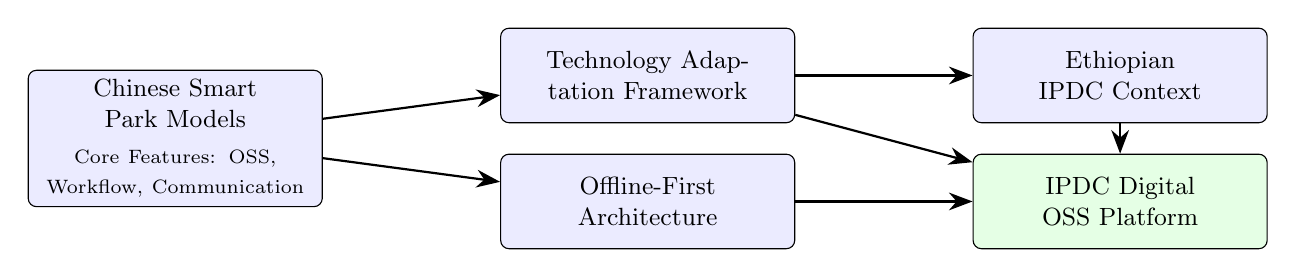
\begin{tikzpicture}[
  block/.style={rectangle, draw, fill=blue!8, text width=3.5cm, text centered, minimum height=1.2cm, rounded corners=3pt, font=\small},
  greenblock/.style={rectangle, draw, fill=green!10, text width=3.5cm, text centered, minimum height=1.2cm, rounded corners=3pt, font=\small},
  arrow/.style={-{Stealth[length=3mm]}, thick}
]
\node[block] (china) at (0,0) {Chinese Smart Park Models\\[2pt]\scriptsize Core Features: OSS, Workflow, Communication};
\node[block] (adapt) at (6,0.8) {Technology Adaptation Framework};
\node[block] (offline) at (6,-0.8) {Offline-First Architecture};
\node[block] (ethiopia) at (12,0.8) {Ethiopian IPDC Context};
\node[greenblock] (platform) at (12,-0.8) {IPDC Digital OSS Platform};

\draw[arrow] (china) -- (adapt);
\draw[arrow] (china) -- (offline);
\draw[arrow] (adapt) -- (ethiopia);
\draw[arrow] (adapt) -- (platform);
\draw[arrow] (offline) -- (platform);
\draw[arrow] (ethiopia) -- (platform);
\end{tikzpicture}}
\caption{Conceptual Framework for Technology Adaptation}
\label{fig:conceptual-framework}
\end{figure}

Chinese smart park experience defines what digital park governance can look like in practice. The adaptation framework answers what can be transferred and what needs rethinking. Offline-first architecture solves the connectivity problem that makes direct replication impossible. The Ethiopian operating environment sets the requirements that all three must satisfy. The IPDC Digital OSS Platform is where those influences converge.

None of the reviewed literature addresses the full combination: complex industrial workflows, multiple stakeholder roles, and variable connectivity. That gap is where this research starts, and the methodology described in the next chapter was designed specifically to work within it.

\chapter{Research Methodology}
\label{ch:methodology}

\section{Introduction}

This chapter describes how the offline-first digital one-stop-shop platform for Ethiopian IPDC was designed, developed, and evaluated. The methodology brings together Design Science Research as the overarching research paradigm with agile-inspired iterative development for building the prototype. The chapter covers the research design, data collection methods, the reasoning behind technology choices, the development approach, and the evaluation framework.

\section{Research Paradigm: Design Science Research}

\subsection{Justification of the DSR Approach}

Design Science Research (DSR) was chosen as the guiding paradigm because of the nature of the research problem itself. IPDC faces a well-documented operational challenge---paper-based service delivery in an environment with unreliable connectivity---and no adequate solution exists. Behavioral methods like surveys or case studies could describe the problem in more detail, but they would not produce the practical artifact needed to actually address it. DSR, on the other hand, is geared toward creating and evaluating purposeful artifacts that solve identified problems while also contributing to the knowledge base \citep{Hevner2004}.

Three features of the research problem make it particularly well suited to DSR. First, the problem is practical and situated within a real organization: IPDC needs a working digital platform, not just a theoretical analysis. Second, the solution calls for creative design rather than routine technology deployment, since no existing system addresses offline-first industrial park governance in African settings. Third, the research aims to produce generalizable knowledge---design principles and an adaptation framework---alongside the specific artifact, which is what distinguishes DSR from ordinary software development \citep{Gregor2013}.

\subsection{DSRM Process Model Application}

The research follows the six-activity DSRM process model proposed by \citet{Peffers2007}. Figure~\ref{fig:dsrm-process} shows how these activities map to the research timeline and thesis structure.

\begin{figure}[H]
\centering
\resizebox{0.95\textwidth}{!}{%
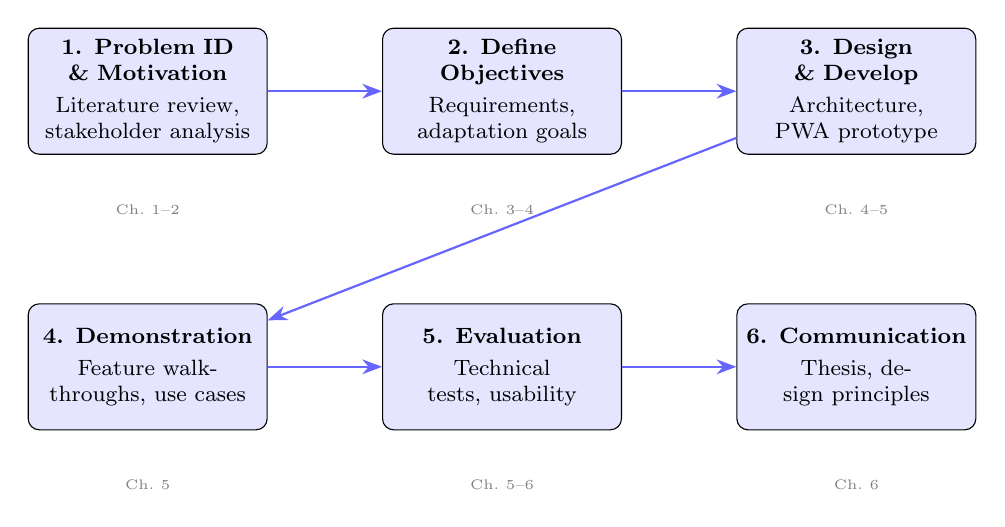
\begin{tikzpicture}[
  activity/.style={rectangle, draw, fill=blue!10, text width=2.8cm, text centered, minimum height=1.6cm, rounded corners=4pt, font=\footnotesize},
  arrow/.style={-{Stealth[length=2.5mm]}, thick, blue!60},
  label/.style={font=\tiny, text=gray}
]
\node[activity] (a1) at (0,0) {\textbf{1. Problem ID \& Motivation}\\[2pt]Literature review, stakeholder analysis};
\node[activity] (a2) at (4.5,0) {\textbf{2. Define Objectives}\\[2pt]Requirements, adaptation goals};
\node[activity] (a3) at (9,0) {\textbf{3. Design \& Develop}\\[2pt]Architecture, PWA prototype};
\node[activity] (a4) at (0,-3.5) {\textbf{4. Demonstration}\\[2pt]Feature walkthroughs, use cases};
\node[activity] (a5) at (4.5,-3.5) {\textbf{5. Evaluation}\\[2pt]Technical tests, usability};
\node[activity] (a6) at (9,-3.5) {\textbf{6. Communication}\\[2pt]Thesis, design principles};

\draw[arrow] (a1) -- (a2);
\draw[arrow] (a2) -- (a3);
\draw[arrow] (a3) -- (a4);
\draw[arrow] (a4) -- (a5);
\draw[arrow] (a5) -- (a6);

\node[label] at (0, -1.5) {Ch.\ 1--2};
\node[label] at (4.5, -1.5) {Ch.\ 3--4};
\node[label] at (9, -1.5) {Ch.\ 4--5};
\node[label] at (0, -5) {Ch.\ 5};
\node[label] at (4.5, -5) {Ch.\ 5--6};
\node[label] at (9, -5) {Ch.\ 6};
\end{tikzpicture}}
\caption{DSRM Process Model Applied to This Research}
\label{fig:dsrm-process}
\end{figure}

\textbf{Activity 1 --- Problem Identification and Motivation} was carried out through a review of the scholarly literature (Chapter~\ref{ch:literature}) and an analysis of current IPDC service delivery processes. The convergence of documented service gaps \citep{Guteta2022, Guteta2023} with the connectivity constraints specific to Ethiopian infrastructure established the importance and urgency of the problem.

\textbf{Activity 2 --- Define Objectives of a Solution} turned the identified problem into concrete design objectives. Through stakeholder requirement gathering and analysis of Chinese smart park reference models, the research defined the functional and non-functional requirements for the platform (detailed in Chapter~\ref{ch:analysis}).

\textbf{Activity 3 --- Design and Development} produced the core artifact: an offline-first PWA prototype built with React, Firebase, and Dexie.js. The architecture was designed to keep services running during connectivity disruptions while supporting workflows that involve multiple stakeholder groups.

\textbf{Activity 4 --- Demonstration} showed the artifact in action through structured walkthroughs of tenant, administrator, and operations workflows, including scenarios that specifically test offline operation.

\textbf{Activity 5 --- Evaluation} assessed the artifact through technical testing of offline functionality, synchronization accuracy, and cross-platform compatibility, along with a usability evaluation based on the System Usability Scale.

\textbf{Activity 6 --- Communication} takes the form of this thesis, which presents the artifact, the reasoning behind its design, evaluation results, and the design principles that emerged from the work.

\section{Research Design Overview}

The overall research design combines qualitative and technical methods within the DSR framework. Qualitative methods---document analysis, platform analysis, and stakeholder requirements gathering---informed the understanding of the problem and shaped design objectives. Technical methods---iterative software development and systematic testing---produced and evaluated the artifact. This mixed approach is consistent with DSR practice, which uses whatever methods are needed to rigorously build and assess the artifact \citep{Hevner2004}.

The work unfolded in four overlapping phases:

\begin{enumerate}
\item \textbf{Exploration Phase} (Months 1--3): Literature review, Chinese platform analysis, stakeholder requirement gathering, and problem formulation.
\item \textbf{Design Phase} (Months 3--5): Architecture design, technology selection, adaptation framework development, and database schema design.
\item \textbf{Development Phase} (Months 4--8): Iterative prototype implementation with features added progressively and offline behavior tested continuously.
\item \textbf{Evaluation Phase} (Months 8--10): Technical testing, usability assessment, and synthesis of design principles.
\end{enumerate}

\section{Data Collection Methods}
\label{sec:data-collection}

\subsection{Stakeholder Requirements Questionnaire}

Structured questionnaires were administered to representatives of the three main stakeholder groups: tenant firm representatives, IPDC administrative staff, and park operations personnel. The questionnaire was designed to capture:

\begin{itemize}
\item Current service delivery workflows and their pain points;
\item How often connectivity disruptions occur and what impact they have;
\item Which services stakeholders most want delivered digitally;
\item Familiarity with technology and patterns of device use;
\item What stakeholders expect from a digital platform.
\end{itemize}

A total of \textbf{49 respondents} completed the questionnaire, exceeding the initial target of 45. Respondents were drawn from \textbf{eleven Special Economic Zones and industrial parks} across Ethiopia: Semera, Hawassa, Adama, Bole Lemi, Mekelle, Kilinto, Kombolcha, Bahir Dar, Debre Birhan, and Jimma SEZs, as well as Dire Dawa Free Trade Zone. This geographic spread ensures that the requirements capture the diversity of park contexts in terms of industry mix, infrastructure maturity, and location. Table~\ref{tab:survey-respondents} summarises the response breakdown by stakeholder group.

\begin{table}[H]
\centering
\caption{Questionnaire Response Summary by Stakeholder Group}
\label{tab:survey-respondents}
\small
\begin{tabular}{lccc}
\toprule
\textbf{Stakeholder Group} & \textbf{Target} & \textbf{Received} & \textbf{Response Rate} \\
\midrule
Tenant Firm Representatives & 20 & 20 & 100\% \\
IPDC Administrative Staff   & 15 & 15 & 100\% \\
Park Operations Personnel   & 10 & 14 & 140\% \\
\midrule
\textbf{Total} & \textbf{45} & \textbf{49} & \textbf{109\%} \\
\bottomrule
\end{tabular}
\end{table}

The questionnaire used Likert-scale items for quantifiable measurement alongside open-ended questions to gather richer qualitative insights. Key findings that directly shaped the platform requirements include the following. On service delivery pain points, the overwhelming majority of tenants reported always needing to follow up on submitted requests, with long wait times, lack of status updates, and difficulty reaching the right person cited as the top three frustrations. Regarding connectivity, most respondents rated internet reliability at their park at 3 out of 5, with outage frequency ranging from ``sometimes (1--2 times per week)'' for field operations staff to ``sometimes (1--4 times per month)'' for administrative staff. On digital readiness, all ten features listed in the platform feature survey received average importance ratings above 4.0 out of 5; offline capability specifically was rated ``5 -- Very Important'' by nearly all respondents across all three groups. Language preference was overwhelmingly ``Both English and Amharic'', directly informing the i18n architecture described in Chapter~\ref{ch:analysis}. On platform adoption intent, only two respondents expressed uncertainty (``Maybe, depending on how easy it is''), while the remainder selected ``Yes, definitely''.

\subsection{Document Analysis}

Existing IPDC documentation was reviewed to understand formal service processes, organizational structures, and regulatory requirements. The documents examined included service request forms, fee schedules, organizational charts, operational guidelines, and annual reports. This analysis fed into the functional requirements and helped ensure that the prototype aligns with established institutional processes.

\subsection{Platform Analysis: WeChat Work and DingTalk}

A systematic analysis of Chinese smart park platforms---primarily WeChat Work and DingTalk---was carried out to identify features, interaction patterns, and architectural approaches that could inform the IPDC platform design. The analysis drew on platform documentation, published research, and publicly available demonstrations. Features were categorized by their relevance and transferability to the Ethiopian context.

This platform analysis served two purposes: it established the source model for the technology adaptation framework, and it provided concrete design inspiration for specific features such as workflow automation, approval routing, and status tracking.

\subsection{Field Observations}

Field visits to IPDC industrial parks gave firsthand insight into service delivery workflows, infrastructure conditions, and user behavior. Observations focused on:

\begin{itemize}
\item How tenants physically interact with administrative offices for service delivery;
\item The technology infrastructure in place (available devices, network quality, power reliability);
\item How different stakeholder groups communicate with one another;
\item Environmental factors that affect technology use (heat, dust, noise in industrial settings).
\end{itemize}

These observations complemented the questionnaire findings by revealing tacit aspects of service delivery that stakeholders might not articulate on their own.

\section{System Development Methodology}

\subsection{Agile-Inspired Iterative Development}

The prototype was developed using an agile-inspired iterative approach. Rather than following a rigid waterfall sequence, development proceeded through multiple iterations, each adding functionality and incorporating lessons from testing. This approach suits DSR well, since the artifact takes shape through an iterative process of design and evaluation \citep{Hevner2004}.

Each iteration followed a build--test--refine cycle:
\begin{enumerate}
\item \textbf{Build:} Implement a set of features drawn from prioritized requirements.
\item \textbf{Test:} Check that everything works, with special attention to offline behavior and cross-platform compatibility.
\item \textbf{Refine:} Fix issues and adjust the design based on what testing revealed.
\end{enumerate}

Iterations were organized around functional modules: authentication and user management; service request workflows; the digital token system; announcements and complaint management; AI model integration; and the interactive park map.

\subsection{Technology Selection Rationale}

Technology choices were guided by three criteria: compatibility with offline-first architectural requirements, maturity and community support for long-term viability, and cost-effectiveness for a thesis research prototype. Table~\ref{tab:tech-stack} summarizes the technologies chosen and the reasoning behind each one.

\begin{table}[H]
\centering
\caption{Technology Stack Summary}
\label{tab:tech-stack}
\small
\begin{tabular}{p{2.2cm}p{3cm}p{6.5cm}}
\toprule
\textbf{Category} & \textbf{Technology} & \textbf{Selection Rationale} \\
\midrule
Frontend Framework & React 19 + TypeScript & Component-based architecture, strong PWA ecosystem, type safety for complex application \\
Build Tool & Vite 7 & Fast development server, native PWA plugin support via vite-plugin-pwa \\
UI Library & Material-UI (MUI) 7 & Comprehensive component library, responsive design, accessibility support \\
Backend & Firebase 12 (Firestore, Auth, Storage) & Built-in offline persistence, generous free tier, real-time synchronization \\
Local Database & Dexie.js 4 (IndexedDB) & High-level IndexedDB wrapper, React hooks integration, query capabilities \\
PWA Tooling & Workbox 7 + vite-plugin-pwa & Industry-standard service worker management, precaching and runtime caching \\
AI Backend & FastAPI (Python) & Lightweight REST API, Pydantic validation, easy model deployment \\
Maps & Leaflet + React-Leaflet & Open-source mapping, no API key required, offline tile caching potential \\
Forms & React Hook Form + Zod & Performant form handling, schema-based validation \\
Charts & Recharts & React-native charting, responsive, minimal dependencies \\
PDF Generation & jsPDF + AutoTable & Client-side PDF generation for invoices and reports \\
\bottomrule
\end{tabular}
\end{table}

\textbf{React and TypeScript} were chosen as the frontend foundation because React's component model supports the modular architecture a multi-stakeholder platform needs, and TypeScript catches type errors at compile time---important for a complex application with eight separate type definition files.

\textbf{Firebase} was preferred over alternatives like Supabase or a custom Node.js backend mainly because of its built-in offline persistence. When Firestore is configured with \texttt{persistentLocalCache()}, it automatically keeps a local copy of accessed data and handles synchronization in both directions. This drastically reduces the engineering effort needed for offline-first behavior compared to building custom synchronization logic from scratch.

\textbf{Dexie.js} complements Firebase's offline capabilities by providing a local database under the application's direct control. It handles operations that need explicit offline queuing, such as service requests submitted while the internet is down. Together, Firestore's transparent cache and Dexie's explicit queue form a dual-layer offline storage architecture.

\textbf{Workbox} was picked for service worker management because it provides well-tested implementations of standard caching strategies (CacheFirst, NetworkFirst, StaleWhileRevalidate) through a declarative configuration. This reduces the risk of service worker bugs that could break offline functionality.

\subsection{Development Tools and Environment}

Development used Visual Studio Code as the primary IDE, with Vite's development server providing hot module replacement for fast iteration. Firebase emulators handled local testing of authentication and Firestore operations without using up cloud resources. The AI model backend was built in Python with FastAPI, and models were trained using scikit-learn and XGBoost on structured datasets representing IPDC operational scenarios.

Version control was managed through Git, with the repository hosted for backup and collaboration. The production build pipeline uses Vite with manual chunk splitting to keep bundle sizes efficient---vendor libraries (React, ReactDOM), the UI framework (Material-UI), and Firebase SDKs are separated into distinct chunks for better caching.

\section{Evaluation Framework}

The prototype evaluation brings together technical assessment and usability evaluation, reflecting the dual nature of what DSR aims to achieve: the artifact needs to both work correctly and be genuinely useful to the people it is built for \citep{Hevner2004}. The evaluation design follows the Framework for Evaluation in Design Science Research (FEDS) proposed by \citet{Venable2016}, which recommends combining formative and summative evaluation strategies.

\subsection{Technical Evaluation}

Technical evaluation checks whether the prototype meets its design specifications, paying special attention to offline-first capabilities. The evaluation covers four dimensions:

\begin{enumerate}
\item \textbf{Offline Functionality:} Each core feature is systematically tested under simulated offline conditions to confirm that users can complete critical workflows without connectivity.
\item \textbf{Synchronization Accuracy:} Data that was created or changed while offline is verified to synchronize correctly with Firestore once connectivity returns, with no data loss or corruption.
\item \textbf{Performance:} Key metrics are measured, including initial load time, cached load time, response time during offline operation, and how long synchronization takes.
\item \textbf{Cross-Platform Compatibility:} The prototype is tested on desktop browsers (Chrome, Firefox), mobile browsers (Chrome for Android, Safari for iOS), and as an installed PWA.
\end{enumerate}

\subsection{Usability Evaluation}

Usability is assessed using the System Usability Scale (SUS), a widely used instrument for measuring perceived system usability \citep{Nielsen1993, Brooke1996}. SUS produces a single score between 0 and 100 based on ten Likert-scale items; scores above 68 are generally considered above average. \citet{Lewis2018} provide a thorough review of the SUS instrument's validity and reliability over three decades of use, confirming its suitability for evaluating novel systems.

The evaluation involves representative stakeholders from each user group (tenants, administrators, operations personnel) who work through structured task scenarios on the prototype and then fill out the SUS questionnaire. Qualitative feedback is also gathered through follow-up questions about specific aspects of the interface and the offline experience.

\subsection{DSR Guidelines Compliance}

As a methodological quality check, the research evaluates its own compliance with Hevner's seven DSR guidelines. Table~\ref{tab:eval-criteria} maps evaluation criteria to the guidelines and specifies what evidence is required.

\begin{table}[H]
\centering
\caption{Evaluation Criteria Matrix}
\label{tab:eval-criteria}
\small
\begin{tabular}{p{3cm}p{4cm}p{5cm}}
\toprule
\textbf{DSR Guideline} & \textbf{Evaluation Criterion} & \textbf{Evidence} \\
\midrule
1. Design as Artifact & Functional prototype exists & Working PWA with documented features \\
2. Problem Relevance & Addresses real IPDC needs & Requirements traced to stakeholder input \\
3. Design Evaluation & Rigorous assessment & Technical tests + SUS usability scores \\
4. Research Contributions & Novel knowledge produced & Adaptation framework + design principles \\
5. Research Rigor & Systematic methods applied & DSRM process followed, documented \\
6. Design as Search & Iterative refinement & Multiple development iterations \\
7. Communication & Results disseminated & Thesis document, chapter structure \\
\bottomrule
\end{tabular}
\end{table}

\section{Ethical Considerations}

The research adheres to ethical principles in several ways. Stakeholder participation in requirement gathering and usability evaluation was voluntary, and participants were told about the purpose of the research and their right to withdraw at any point. No personally identifiable data from real IPDC tenants or staff was used in the prototype; all demonstration data is synthetic. The authentication system stores credentials securely through Firebase Authentication, and offline credential caching uses hashing rather than plaintext storage.

The research also considers the ethical implications of introducing technology into an organizational context. The platform is designed to support and enhance human roles, not replace them---administrative staff remain at the center of service delivery, with the platform giving them better tools rather than automating them out of the picture.

\section{Chapter Summary}

This chapter laid out the research methodology, with Design Science Research as the overarching paradigm and the DSRM process model organizing the work into six activities from problem identification through to communication. Data collection drew on stakeholder questionnaires, document analysis, Chinese platform analysis, and field observations, while development followed agile-inspired iterations with technology choices driven by offline-first requirements. The evaluation framework combines technical assessment of offline functionality, synchronization, and performance with SUS usability evaluation and Hevner's DSR guidelines compliance. The next chapter presents the system analysis and design, covering stakeholder requirements, the China-to-Ethiopia adaptation framework, and the resulting system architecture.

\chapter{System Analysis and Design}
\label{ch:analysis}

\section{Introduction}

Getting from stakeholder pain points to a working system design is rarely a linear process. This chapter records what that process produced for the IPDC platform: the requirements that emerged from stakeholder analysis, the framework for adapting Chinese smart park patterns to the Ethiopian context, and the architecture that resulted. Not every decision was obvious at the time --- but all of them trace back to a documented constraint or a real operational need.

\section{Requirements Analysis}

\subsection{Stakeholder Identification and Analysis}

Organizational analysis of IPDC's structure, combined with insights from the stakeholder questionnaires, identified four distinct stakeholder groups, each with its own role, priorities, and interaction patterns.

\textbf{Tenant Enterprises} are the primary consumers of services. Their representatives --- typically operations managers and administrative staff --- submit service requests, track progress, handle fee payments, and raise complaints. Speed, transparency, and the ability to keep working during connectivity outages are their chief concerns.

\textbf{IPDC Administrative Staff} serve as the bridge between tenants and operational resources. Service coordinators, permit officers, and finance officers process requests, publish announcements, manage tenant accounts, and resolve complaints. Workflow efficiency and dependable record-keeping matter most to this group.

\textbf{Operations Personnel} are the ones doing the physical work once a request is approved. A maintenance coordinator might receive a task assignment, find they cannot access the system from a remote corner of the park, and need to pick it back up an hour later. That specific scenario --- task received, connectivity lost, work continues --- is exactly what the mobile offline task queue was built for.

\textbf{IPDC Management} needs a high-level view of operational performance without involvement in day-to-day platform use. Directors and planning officers rely on aggregated data about service volumes, resolution times, and resource utilization to inform decisions.

\subsection{Functional Requirements}

Table~\ref{tab:func-req} summarizes the twelve functional requirement groups that emerged from stakeholder analysis and the mapping of Chinese smart park features.

\begin{table}[H]
\centering
\caption{Functional Requirements Summary}
\label{tab:func-req}
\small
\begin{tabular}{lp{3.5cm}p{7.5cm}}
\toprule
\textbf{ID} & \textbf{Requirement} & \textbf{Description} \\
\midrule
FR1 & User Authentication & Email-based registration and login with role assignment (tenant, admin, operations); offline authentication fallback using cached credentials \\
FR2 & Service Request Management & Submit, track, approve, and complete service requests across multiple categories with file attachments and priority levels \\
FR3 & Digital Service Token System & Internal credit system for fee tracking with tiered accounts (basic, silver, gold, platinum), transaction history, and automated deductions \\
FR4 & Announcement Management & Create, distribute, and display system announcements targeted to specific audiences with priority and expiration settings \\
FR5 & Complaint Management & File complaints against completed services with evidence uploads, track resolution through defined workflows \\
FR6 & Asset \& Maintenance Management & Register, categorize, and track park assets; schedule and record maintenance activities \\
FR7 & AI-Powered Services & Automated service request classification, predictive equipment maintenance, and intelligent park recommendation for prospective tenants \\
FR8 & Document Management & Upload, store, and retrieve documents associated with service requests and OSS applications \\
FR9 & OSS Services & Digital interfaces for investment permits, business licenses, customs services, and banking coordination \\
FR10 & Interactive Park Map & Geographic visualization of Ethiopian industrial parks with detail overlays \\
FR11 & Billing \& Invoicing & Generate invoices, track payment transactions, and export PDF reports \\
FR12 & Notifications & In-platform and email notifications for status changes and announcements \\
\bottomrule
\end{tabular}
\end{table}

\subsection{Non-Functional Requirements}

Table~\ref{tab:nonfunc-req} sets out the non-functional requirements that constrain and shape the system architecture.

\begin{table}[H]
\centering
\caption{Non-Functional Requirements}
\label{tab:nonfunc-req}
\small
\begin{tabular}{lp{3cm}p{8cm}}
\toprule
\textbf{ID} & \textbf{Requirement} & \textbf{Specification} \\
\midrule
NFR1 & Offline-First Operation & All core workflows (FR1--FR5) must function without connectivity; data persists locally and synchronizes when online \\
NFR2 & Cross-Platform Access & Single codebase accessible on desktop, tablet, and mobile via web browser; installable as PWA on mobile devices \\
NFR3 & Response Time & Page transitions under 2 seconds; form submissions under 1 second in offline mode \\
NFR4 & Sync Latency & Queued data synchronized within 30 seconds of connectivity restoration \\
NFR5 & Security & Role-based access control; Firebase Authentication; credential hashing for offline cache \\
NFR6 & Scalability & Architecture supports multiple industrial parks under a single deployment \\
NFR7 & Accessibility & WCAG 2.1 Level AA compliance for core interfaces \\
\bottomrule
\end{tabular}
\end{table}

\subsection{MoSCoW Prioritization}

The MoSCoW framework guided requirement prioritization and iteration planning. Offline availability served as the primary deciding factor. Table~\ref{tab:moscow} shows the results.

\begin{table}[H]
\centering
\caption{MoSCoW Feature Prioritization}
\label{tab:moscow}
\small
\begin{tabular}{p{2.5cm}p{5cm}p{4cm}}
\toprule
\textbf{Priority} & \textbf{Features} & \textbf{Offline Requirement} \\
\midrule
Must Have & Authentication, service requests, token system, announcements, complaint management & Full offline capability \\
Should Have & Asset management, notifications, billing, document management & Graceful degradation \\
Could Have & AI services, interactive map, OSS services, PDF export & Online-preferred \\
Won't Have (this phase) & External payment gateway, IoT integration, Amharic localization & Identified as future work \\
\bottomrule
\end{tabular}
\end{table}

\section{China-to-Ethiopia Technology Adaptation Framework}

\subsection{Chinese Smart Park Feature Analysis}

An examination of WeChat Work and DingTalk platforms revealed several feature categories common to Chinese smart parks: enterprise messaging and group communication, workflow approval routing, service request submission and tracking, payment processing (through WeChat Pay or Alipay), document management, attendance and access control, video conferencing, and analytics dashboards.

\subsection{Adaptation Dimensions}

Four dimensions structure the adaptation framework. The technological dimension carries the most weight --- the connectivity gap between Chinese and Ethiopian contexts is the primary constraint that reshapes everything else --- but organizational fit, cultural context, and economic realities each produce their own distinct adaptation requirements.

\textbf{Technological Dimension:} Connectivity demands the most fundamental adaptation. Chinese platforms assume persistent high-speed internet; the Ethiopian version replaces this with an offline-first architecture. Dependencies on Chinese ecosystem platforms (WeChat, Alipay, Alibaba Cloud) are replaced by globally accessible alternatives (Firebase, web standards).

\textbf{Organizational Dimension:} IPDC's organizational structure and service processes do not mirror those of Chinese park management. The adaptation translates Chinese workflow patterns into IPDC's three-role structure (tenant, admin, operations) and aligns approval workflows with the institution's existing hierarchies.

\textbf{Cultural Dimension:} Interface design was adjusted to fit local expectations. An English-language interface reflects the international business environment of Ethiopian industrial parks, while Amharic localization has been identified as a future enhancement. The digital service token concept is an adaptation of Chinese integrated payment, designed for a context where external payment gateway partnerships have not yet been established.

\textbf{Economic Dimension:} Cost constraints shaped technology choices at every stage: PWA over native apps (eliminating app store fees and multi-platform development costs), Firebase's free tier over paid cloud services, and open-source tools across the full stack.

\subsection{Feature Mapping and Modification Matrix}

Table~\ref{tab:adaptation-matrix} maps each Chinese smart park feature to its adapted counterpart in the IPDC platform.

\begin{table}[H]
\centering
\caption{China-to-Ethiopia Feature Adaptation Matrix}
\label{tab:adaptation-matrix}
\small
\begin{tabular}{p{3.5cm}p{3.5cm}p{5cm}}
\toprule
\textbf{Chinese Feature} & \textbf{IPDC Adaptation} & \textbf{Modification Rationale} \\
\midrule
WeChat Work messaging & Announcement system & Structured notifications replace real-time chat; works offline \\
DingTalk approval workflows & Service request pipeline & Adapted to tenant$\rightarrow$admin$\rightarrow$operations flow \\
WeChat Pay / Alipay & Digital service tokens & Internal system avoids external API dependency \\
Native mobile apps & Progressive Web App & Single codebase, no app store, offline-capable \\
Cloud-only architecture & Offline-first with Firebase & Dual-layer local storage + cloud sync \\
Real-time IoT monitoring & Asset management module & Manual tracking as IoT infrastructure unavailable \\
Chinese language UI & English interface & Primary business language; Amharic as future work \\
Alibaba Cloud backend & Firebase (Google Cloud) & Global availability, built-in offline persistence \\
\bottomrule
\end{tabular}
\end{table}

\subsection{Offline-First Adaptation Strategy}

The offline-first adaptation represents the most architecturally consequential departure from the Chinese reference models. It is worth being clear that this is not simply a matter of enabling a ``save offline'' toggle; it requires rethinking how data flows through the entire system. The adaptation is built on three guiding principles:

\begin{enumerate}
\item \textbf{Local-first data storage:} Every piece of data the user reads comes from local storage (the Firestore cache or IndexedDB), while network requests happen in the background to keep things synchronized.
\item \textbf{Queue-based write operations:} When users create or modify data while offline, their operations are placed in an IndexedDB queue and executed against Firestore once connectivity is restored.
\item \textbf{Transparent status communication:} The interface continuously shows connectivity status, synchronization state, and any pending operations, so users always know exactly where their data stands.
\end{enumerate}

\section{System Architecture}

\subsection{High-Level Architecture Overview}

The platform is organized as a three-tier architecture adapted for offline-first operation. Figure~\ref{fig:architecture} provides an overview of the high-level structure.

\begin{figure}[H]
\centering
\resizebox{0.95\textwidth}{!}{%
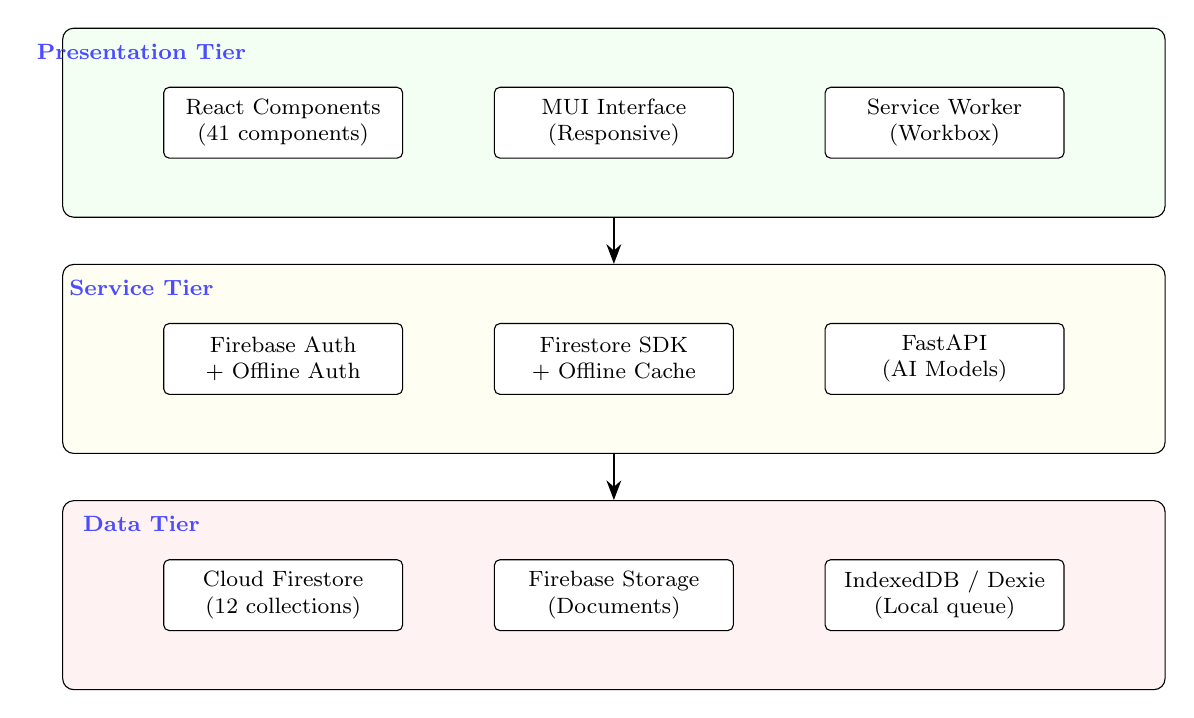
\begin{tikzpicture}[
  tier/.style={rectangle, draw, fill=blue!5, minimum width=14cm, minimum height=2.4cm, rounded corners=4pt},
  component/.style={rectangle, draw, fill=white, text width=2.8cm, text centered, minimum height=0.9cm, font=\footnotesize, rounded corners=2pt},
  arrow/.style={-{Stealth[length=2.5mm]}, thick},
  label/.style={font=\footnotesize\bfseries, text=blue!70}
]

% Presentation Tier
\node[tier, fill=green!5] (pres) at (0,4.5) {};
\node[label] at (-6,5.4) {Presentation Tier};
\node[component] at (-4.2,4.5) {React Components\\(41 components)};
\node[component] at (0,4.5) {MUI Interface\\(Responsive)};
\node[component] at (4.2,4.5) {Service Worker\\(Workbox)};

% Service Tier
\node[tier, fill=yellow!5] (serv) at (0,1.5) {};
\node[label] at (-6,2.4) {Service Tier};
\node[component] at (-4.2,1.5) {Firebase Auth\\+ Offline Auth};
\node[component] at (0,1.5) {Firestore SDK\\+ Offline Cache};
\node[component] at (4.2,1.5) {FastAPI\\(AI Models)};

% Data Tier
\node[tier, fill=red!5] (data) at (0,-1.5) {};
\node[label] at (-6,-0.6) {Data Tier};
\node[component] at (-4.2,-1.5) {Cloud Firestore\\(12 collections)};
\node[component] at (0,-1.5) {Firebase Storage\\(Documents)};
\node[component] at (4.2,-1.5) {IndexedDB / Dexie\\(Local queue)};

\draw[arrow] (pres) -- (serv);
\draw[arrow] (serv) -- (data);

\end{tikzpicture}}
\caption{High-Level System Architecture}
\label{fig:architecture}
\end{figure}

The \textbf{Presentation Tier} comprises 41 React components across six modules (admin, common, layout, map, operations, tenant) and 15 page-level components. Material-UI supplies the responsive design system; Workbox handles service worker management for asset caching and offline navigation.

The \textbf{Service Tier} mediates between the user interface and persistent storage. Firebase Authentication handles online identity verification, backed by an offline authentication module that checks cached credentials stored in IndexedDB. The Firestore SDK provides transparent offline caching, and a custom sync service manages the explicit operation queue. Separately, the FastAPI backend serves three AI models through REST endpoints.

The \textbf{Data Tier} blends cloud and local storage. Cloud Firestore holds twelve collections constituting the complete data model. Firebase Storage retains uploaded documents and images. IndexedDB (through Dexie.js) maintains a local queue of pending operations and cached service request data for offline access.

\subsection{Offline-First Architecture Design}

The offline-first architecture relies on a dual-layer storage strategy. Figure~\ref{fig:offline-flow} shows data flow during a service request submission under both online and offline conditions.

\begin{figure}[H]
\centering
\resizebox{0.85\textwidth}{!}{%
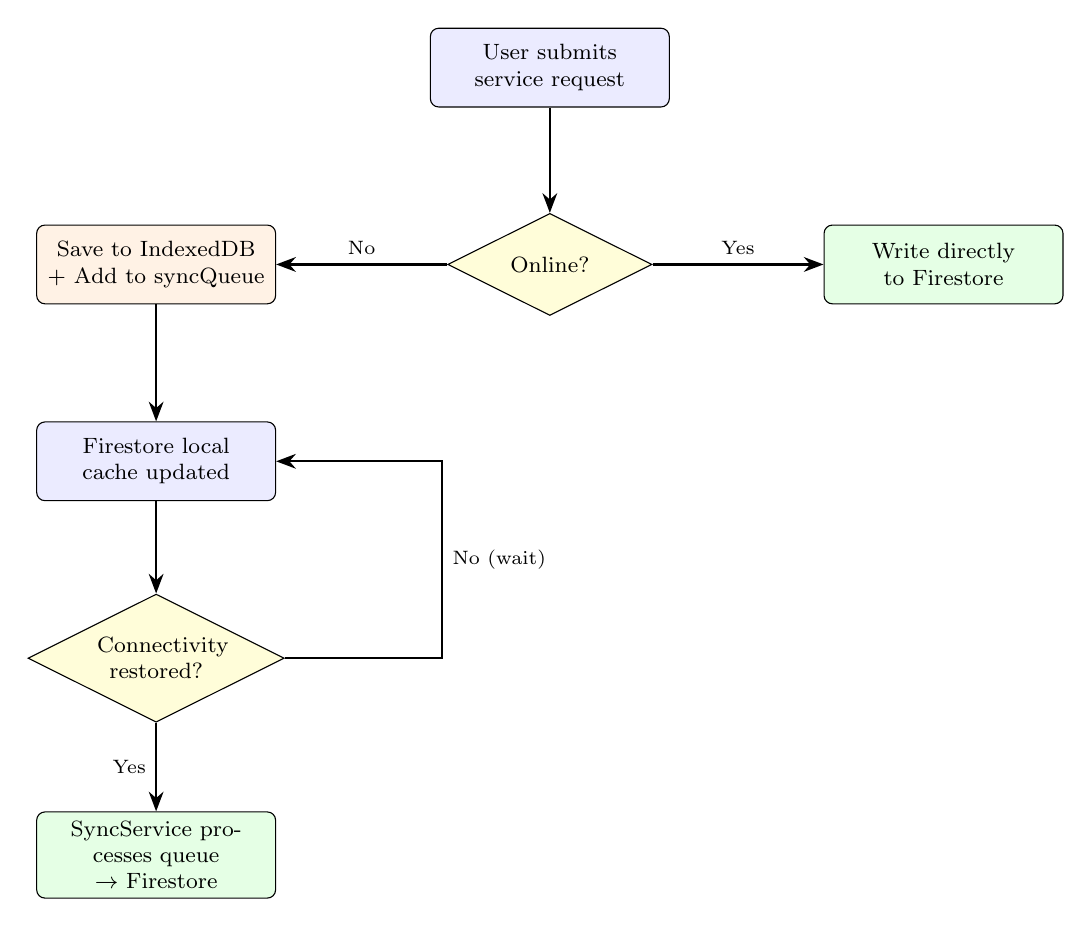
\begin{tikzpicture}[
  box/.style={rectangle, draw, fill=blue!8, text width=2.8cm, text centered, minimum height=1cm, rounded corners=3pt, font=\footnotesize},
  decision/.style={diamond, draw, fill=yellow!15, text width=1.5cm, text centered, aspect=2, font=\footnotesize},
  arrow/.style={-{Stealth[length=2.5mm]}, thick},
]

\node[box] (user) at (0,0) {User submits service request};
\node[decision] (check) at (0,-2.5) {Online?};
\node[box, fill=green!10] (direct) at (5,-2.5) {Write directly to Firestore};
\node[box, fill=orange!10] (queue) at (-5,-2.5) {Save to IndexedDB\\+ Add to syncQueue};
\node[box] (cache) at (-5,-5) {Firestore local cache updated};
\node[decision] (reconnect) at (-5,-7.5) {Connectivity restored?};
\node[box, fill=green!10] (sync) at (-5,-10) {SyncService processes queue $\rightarrow$ Firestore};

\draw[arrow] (user) -- (check);
\draw[arrow] (check) -- node[above]{\scriptsize Yes} (direct);
\draw[arrow] (check) -- node[above]{\scriptsize No} (queue);
\draw[arrow] (queue) -- (cache);
\draw[arrow] (cache) -- (reconnect);
\draw[arrow] (reconnect) -- node[left]{\scriptsize Yes} (sync);
\draw[arrow] (reconnect.east) -- ++(2,0) |- node[near start, right]{\scriptsize No (wait)} (cache.east);

\end{tikzpicture}}
\caption{Offline-First Data Flow for Service Request Submission}
\label{fig:offline-flow}
\end{figure}

\textbf{Layer 1 --- Firebase Firestore Persistent Cache:} With \texttt{persistentLocalCache()} and \texttt{persistentMultipleTabManager()} enabled, Firestore maintains a local copy of every document the user has previously accessed. When offline, read operations draw from this cache, giving users seamless access to existing records without any network connection.

\textbf{Layer 2 --- Dexie.js IndexedDB Queue:} Write operations initiated while offline are stored in two IndexedDB tables managed by Dexie.js. The \texttt{serviceRequests} table holds complete request data locally; the \texttt{syncQueue} table records metadata for each pending operation (type, collection, document ID, timestamp). Once the \texttt{useOnlineStatus} hook detects restored connectivity, the sync service processes queued items and writes them to Firestore.

\subsection{PWA Architecture}

The PWA setup, managed through vite-plugin-pwa, employs three caching strategies:

\begin{itemize}
\item \textbf{Precaching:} JavaScript bundles, CSS stylesheets, HTML pages, icons, and image assets are cached when the service worker is first installed, ensuring the application shell loads even without network access.
\item \textbf{CacheFirst} (Google Fonts): Font resources are served from cache with a one-year expiration, avoiding unnecessary repeat downloads.
\item \textbf{NetworkFirst} (Firebase Storage, API endpoints): For dynamic content, the application tries the network first and falls back to cached versions during outages. Firebase Storage responses are cached for seven days.
\end{itemize}

The web app manifest declares the application as \texttt{"display": "standalone"}, enabling full-screen installation on mobile devices. It also specifies the application name (``IPDC-OSS Platform''), a theme color (\texttt{\#2563eb}), and icon assets at 192px and 512px resolutions.

\subsection{Authentication Architecture}

Authentication follows a dual-mode design so that users can still log in during connectivity disruptions. Figure~\ref{fig:auth-flow} illustrates the authentication flow.

\begin{figure}[H]
\centering
\resizebox{0.95\textwidth}{!}{%
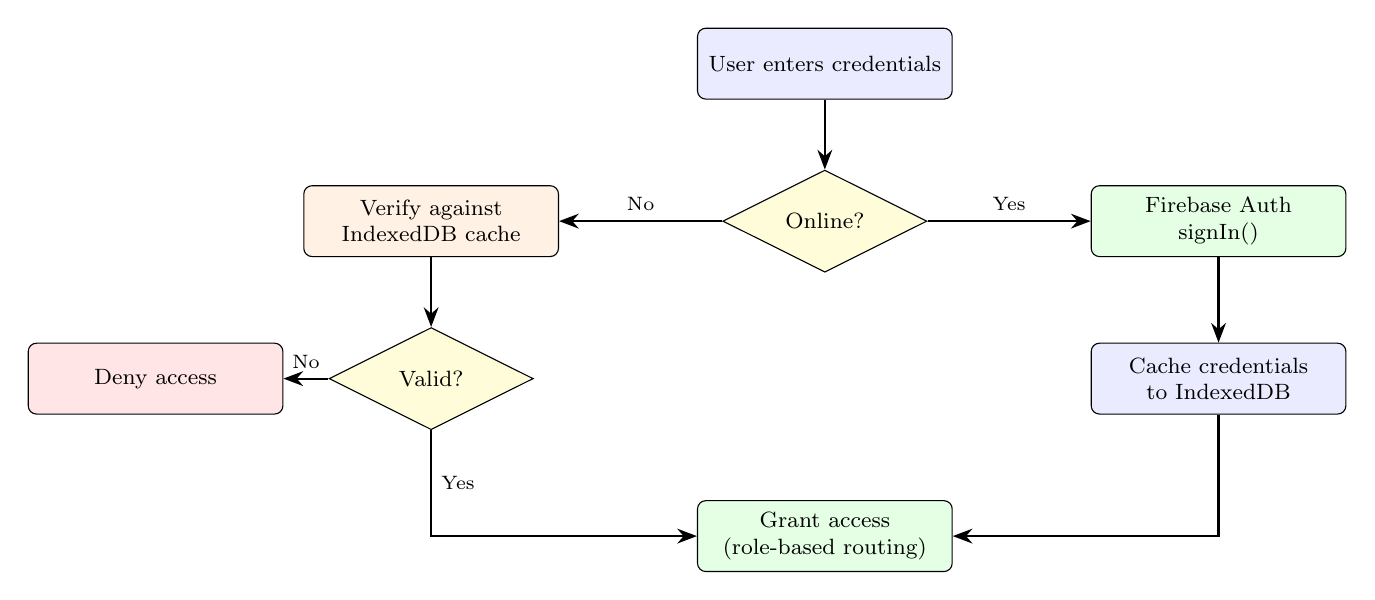
\begin{tikzpicture}[
  box/.style={rectangle, draw, fill=blue!8, text width=3cm, text centered, minimum height=0.9cm, rounded corners=3pt, font=\footnotesize},
  decision/.style={diamond, draw, fill=yellow!15, text width=1.5cm, text centered, aspect=2, font=\footnotesize},
  arrow/.style={-{Stealth[length=2.5mm]}, thick},
]

\node[box] (login) at (0,0) {User enters credentials};
\node[decision] (online) at (0,-2) {Online?};
\node[box, fill=green!10] (firebase) at (5,-2) {Firebase Auth\\signIn()};
\node[box] (cache) at (5,-4) {Cache credentials to IndexedDB};
\node[box, fill=orange!10] (offline) at (-5,-2) {Verify against IndexedDB cache};
\node[decision] (valid) at (-5,-4) {Valid?};
\node[box, fill=green!10] (grant) at (0,-6) {Grant access\\(role-based routing)};
\node[box, fill=red!10] (deny) at (-8.5,-4) {Deny access};

\draw[arrow] (login) -- (online);
\draw[arrow] (online) -- node[above]{\scriptsize Yes} (firebase);
\draw[arrow] (firebase) -- (cache);
\draw[arrow] (cache) |- (grant);
\draw[arrow] (online) -- node[above]{\scriptsize No} (offline);
\draw[arrow] (offline) -- (valid);
\draw[arrow] (valid) |- node[near start, right]{\scriptsize Yes} (grant);
\draw[arrow] (valid) -- node[above]{\scriptsize No} (deny);

\end{tikzpicture}}
\caption{Dual-Mode Authentication Flow}
\label{fig:auth-flow}
\end{figure}

When online, authentication proceeds through Firebase Auth via \texttt{signInWithEmailAndPassword()}. After a successful login, credentials are hashed and stored in IndexedDB through the \texttt{cacheCredentials()} utility. When offline, the system retrieves cached credentials and checks the user's input against the stored hash. The \texttt{AuthContext} component orchestrates this dual-mode logic, switching automatically to offline authentication whenever it encounters network errors.

Three user roles --- \texttt{tenant}, \texttt{admin}, and \texttt{operations} --- determine which dashboard a user sees and which features they can access, managed through role-based conditional rendering in the React component tree.

\subsection{AI Integration Architecture}

Three machine learning models are served through a FastAPI backend as REST endpoints at \texttt{/api/v1/}:

\begin{enumerate}
\item \textbf{Service Classifier} (\texttt{/classify-service}): Accepts a request title and description; returns a predicted service type, priority level, estimated processing time in days, confidence score, and contextual recommendations.
\item \textbf{Predictive Maintenance} (\texttt{/predict-maintenance}): Takes asset attributes --- age, condition score, maintenance history --- and outputs a failure probability, risk level, estimated days until failure, and a recommended action. The output is designed to give operations teams something actionable rather than just a probability number.
\item \textbf{Park Recommendation} (\texttt{/recommend-parks}): Accepts a tenant profile (industry sector, employee count, investment capital, infrastructure needs); returns ranked park recommendations with match scores, pros and cons, and cost estimates. Scoring weights are: industry alignment 30\%, capacity 25\%, infrastructure 20\%, cost 15\%, location 10\%.
\end{enumerate}

AI features are designed with graceful degradation: when the FastAPI backend is unreachable during connectivity outages, the platform reverts to manual classification and disables recommendation features without blocking core workflows.

\section{Database Design}

\subsection{Firestore Collections Schema}

The Firestore database is organized into twelve collections. Table~\ref{tab:firestore-schema} documents the primary collections with their key fields and purposes.

\begin{table}[H]
\centering
\caption{Firestore Collections Schema}
\label{tab:firestore-schema}
\small
\begin{tabular}{p{3cm}p{5cm}p{4cm}}
\toprule
\textbf{Collection} & \textbf{Key Fields} & \textbf{Purpose} \\
\midrule
users & uid, email, displayName, role, parkId, createdAt & User profiles and roles \\
serviceRequests & id, tenantId, title, description, serviceType, priority, status, assignedTo & Core service workflow \\
ossServiceRequests & id, tenantId, serviceCategory, documents[], status & OSS-specific requests \\
announcements & id, title, content, targetAudience, priority, expiresAt, isActive & System announcements \\
complaints & id, requestId, tenantId, category, evidence[], status, resolution & Complaint tracking \\
tokenAccounts & tenantId, balance, tier, totalEarned, totalSpent & Token balances \\
tokenTransactions & id, tenantId, type, amount, description, timestamp & Transaction ledger \\
invoices & id, tenantId, lineItems[], total, status, pdfUrl & Billing records \\
paymentTransactions & id, tenantId, amount, method, referenceNumber & Payment tracking \\
assets & id, name, category, condition, purchaseCost, currentValue & Park asset inventory \\
maintenanceRecords & id, assetId, type, scheduledDate, completedDate, cost & Maintenance history \\
notifications & id, userId, title, message, read, createdAt & User notifications \\
\bottomrule
\end{tabular}
\end{table}

\subsection{IndexedDB Schema (Dexie.js)}

The local IndexedDB database, named \texttt{IPDCDatabase}, holds two tables tailored for offline operations:

\begin{itemize}
\item \texttt{serviceRequests}: Stores complete request documents for offline access. Indexed on: \texttt{id}, \texttt{tenantId}, \texttt{status}, \texttt{priority}, \texttt{serviceType}, \texttt{createdAt}.
\item \texttt{syncQueue}: Stores pending write operations with auto-incrementing IDs. Indexed on: \texttt{++id}, \texttt{type}, \texttt{collection}, \texttt{status}, \texttt{createdAt}.
\end{itemize}

The sync queue recognizes four status values: \texttt{pending} (awaiting sync), \texttt{syncing} (currently being processed), \texttt{synced} (successfully written to Firestore), and \texttt{failed} (sync attempted but unsuccessful; will be retried).

\section{User Interface Design}

\subsection{Design Principles}

The interface follows Material Design guidelines through the MUI component library, enhanced with a custom theme. A primary color (\texttt{\#2563eb}, professional blue) and secondary color (\texttt{\#059669}, confident green) establish a visual identity suited to an institutional platform. Status-specific colors give instant feedback: amber for pending, blue for approved, purple for in-progress, green for completed, and red for rejected.

Responsive breakpoints at 600px and 960px ensure the platform works across device categories. The \texttt{useDeviceDetection} hook dynamically adjusts layout density and navigation patterns based on the device in use.

\subsection{Navigation and Role-Based Views}

After authentication, the routing system directs each user to a role-appropriate dashboard:

\begin{itemize}
\item \textbf{Tenant Dashboard:} Service request submission, request tracking, token management, complaint filing, park recommendations.
\item \textbf{Admin Dashboard:} Request management (across all tenants), announcement creation, tenant account management, complaint resolution, billing oversight, asset management.
\item \textbf{Operations Dashboard:} Service fulfillment, maintenance scheduling, asset inspection, performance metrics.
\end{itemize}

\subsection{Status Indicators}

The \texttt{StatusBar} component keeps users informed about system state at all times, showing:
\begin{itemize}
\item Online/offline connectivity status with a color-coded indicator;
\item Device type (desktop, tablet, or mobile);
\item Number of pending sync operations;
\item Timestamp of the last successful synchronization.
\end{itemize}

This transparency is essential for an offline-first system, where users need to know whether their actions have been synchronized to the server or are still waiting in a local queue.

\section{Chapter Summary}

The analysis and design work described in this chapter produced several concrete outputs: twelve functional and seven non-functional requirement groups grounded in stakeholder input, a four-dimension adaptation framework translating Chinese platform patterns to the Ethiopian context, and a three-tier architecture built from 41 React components, Firebase and FastAPI services, and a dual-layer local storage strategy. Of these, the dual-mode authentication and queue-based synchronization mechanisms arguably matter most to end users --- they are what make the platform feel continuous and trustworthy rather than intermittent and fragile. It is also worth noting that many of the design decisions recorded here were not obvious at the outset; they emerged iteratively as the constraints of the Ethiopian operating environment became clearer. How those decisions translate into working software, and what the evaluation reveals about them, is the subject of the next chapter.

\chapter{Implementation and Evaluation}
\label{ch:implementation}

\section{Introduction}

This chapter is, in many ways, where the design decisions of the previous chapter either hold up or fall apart. What was built is a working Progressive Web Application comprising roughly 105 TypeScript source files, three trained machine learning models, and a dual-layer offline data management architecture. Whether it actually works as intended is the question the evaluation half of this chapter answers --- through offline functionality tests, performance measurement, cross-platform compatibility checks, and a structured usability assessment with nine real IPDC stakeholders.

\section{Development Environment and Tools}

\subsection{Development Setup}

The development environment centered on Visual Studio Code as the primary IDE, Node.js (v18+) as the JavaScript runtime, React 19.2.1 \citep{React2024} as the frontend framework, and the Vite development server for hot module replacement at \texttt{localhost:5173}. Firebase emulators handled local testing of authentication and Firestore operations, avoiding unnecessary consumption of cloud quotas. The AI model backend was developed separately in a Python environment using FastAPI, with models available at \texttt{localhost:8000}.

\subsection{Project Structure}

The project follows a modular directory structure organized by concern. Application source code lives in \texttt{src/}, while machine learning components and the API server reside in \texttt{ai-models/}. Table~\ref{tab:project-structure} provides an overview of the directory layout and component counts.

\begin{table}[H]
\centering
\caption{Project Directory Structure and Component Counts}
\label{tab:project-structure}
\small
\begin{tabular}{p{3.8cm}p{7.5cm}l}
\toprule
\textbf{Directory} & \textbf{Purpose} & \textbf{Files} \\
\midrule
src/components/admin/ & Admin-specific UI components & 6 \\
src/components/common/ & Shared UI components (StatusBar, FileUpload, etc.) & 12 \\
src/components/layout/ & Navigation and layout scaffolding & 3 \\
src/components/map/ & Interactive park map and details & 3 \\
src/components/operations/ & Operations module components & 4 \\
src/components/tenant/ & Tenant-specific components & 13 \\
src/pages/ & Page-level route components & 15 \\
src/services/ & Business logic and API services & 18 \\
src/services/offline/ & Offline storage and sync services & 3 \\
src/contexts/ & React context providers & 1 \\
src/hooks/ & Custom React hooks & 4 \\
src/db/ & Dexie.js schema definition & 1 \\
src/types/ & TypeScript type definitions & 8 \\
src/config/ & Firebase and theme configuration & 2 \\
ai-models/ & Three ML models + FastAPI backend & 12 \\
\midrule
\textbf{Total} & & \textbf{$\sim$105} \\
\bottomrule
\end{tabular}
\end{table}

\subsection{Build and Deployment Configuration}

The Vite build uses manual chunk splitting (\texttt{vendor}, \texttt{mui}, \texttt{firebase}) so application updates do not invalidate cached library bundles --- valuable where connectivity is limited.

The vite-plugin-pwa generates the service worker and web app manifest automatically from the configuration in \texttt{vite.config.ts}. The deployed platform is accessible at the following URLs:

\begin{itemize}
  \item \textbf{Frontend Application:} \url{https://ipdc-oss-platform.vercel.app/} --- deployed on Vercel with HTTPS, global CDN distribution, and automatic SSL certificate management.
  \item \textbf{AI Backend API:} \url{https://ipdc-oss-platform.onrender.com/api/docs} --- deployed on Render, hosting the FastAPI server with the three trained ML models. Interactive API documentation (Swagger UI) is available at this URL; model endpoints are served under the \texttt{/api/v1/} prefix (e.g., \texttt{/api/v1/classify-service}, \texttt{/api/v1/predict-maintenance}, \texttt{/api/v1/recommend-parks}).
\end{itemize}

\section{Key Feature Implementation}

\subsection{Offline-First Architecture Implementation}

The offline-first architecture is realized through three cooperating subsystems: Firebase Firestore's transparent cache, the Dexie.js local database, and a custom synchronization service.

\textbf{Firebase Offline Persistence} is activated in the Firebase configuration module (\texttt{src/config/firebase.ts}) during initialization:

\begin{lstlisting}[language=Java, caption={Firebase Offline Persistence Configuration}, label={lst:firebase-config}]
initializeFirestore(app, {
  localCache: persistentLocalCache({
    tabManager: persistentMultipleTabManager()
  })
});
\end{lstlisting}

This instructs Firestore to maintain a persistent local cache of all documents the user has accessed, keeping it intact across browser sessions and coordinating access when multiple tabs are open. When the network is unavailable, reads are served from this cache and writes are internally queued for later synchronization.

\textbf{Dexie.js Local Database} extends Firestore's cache with explicit offline data management. The schema, defined in \texttt{src/db/schema.ts}, sets up two indexed tables:

\begin{lstlisting}[language=Java, caption={Dexie.js Database Schema}, label={lst:dexie-schema}]
const db = new Dexie('IPDCDatabase');
db.version(1).stores({
  serviceRequests:
    'id, tenantId, status, priority, serviceType, createdAt',
  syncQueue:
    '++id, type, collection, status, createdAt'
});
\end{lstlisting}

\textbf{The Sync Service} (\texttt{src/services/offline/syncService.ts}) picks up queued items once connectivity is detected. It iterates through pending entries, converts local JavaScript \texttt{Date} objects to Firestore \texttt{Timestamp} objects, writes to the appropriate collection, and marks each item with an updated status. A built-in retry mechanism handles transient failures so no queued data is lost.

\subsection{Authentication with Offline Fallback}

The authentication system implements the dual-mode design outlined in Chapter~\ref{ch:analysis}. The \texttt{AuthContext} (\texttt{src/contexts/AuthContext.tsx}) wraps the entire application and manages authentication state. When signing in online, credentials are verified through Firebase Auth and cached locally:

\begin{lstlisting}[language=Java, caption={Credential Caching After Online Authentication}, label={lst:auth-cache}]
// After successful Firebase Auth sign-in:
await cacheCredentials(email, password);
await cacheAuthState({
  uid: user.uid,
  email: user.email,
  displayName: user.displayName,
  role: userData.role
});
\end{lstlisting}

If the sign-in attempt fails because of a network error, the context automatically falls back to offline verification:

\begin{lstlisting}[language=Java, caption={Offline Authentication Fallback}, label={lst:auth-offline}]
// Network error detected during sign-in:
const isValid = await verifyOfflineCredentials(email, password);
if (isValid) {
  const cachedUser = await getCachedAuthState();
  // Grant access using cached user profile
}
\end{lstlisting}

Any user who has previously authenticated while online can therefore continue using the platform during connectivity outages. Figure~\ref{fig:auth-interfaces} shows the sign-in and tenant registration interfaces.

\begin{figure}[H]
\centering
\begin{minipage}[t]{0.48\textwidth}
\centering
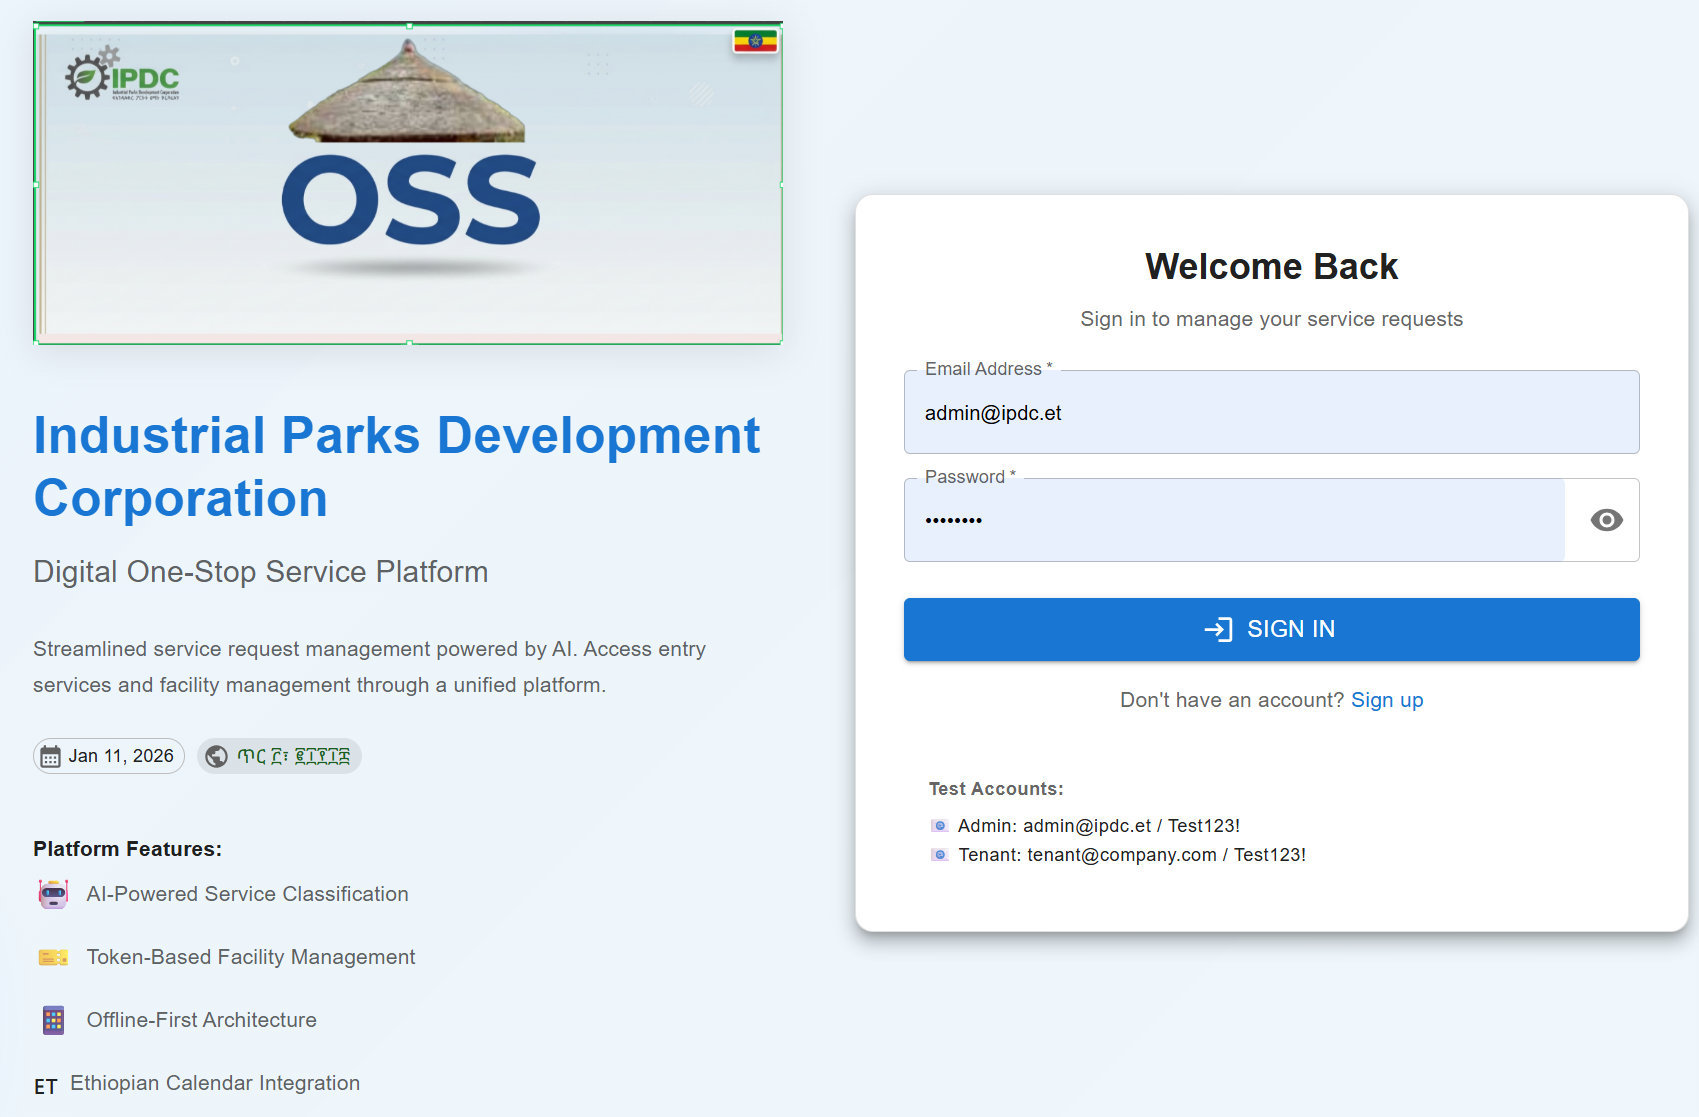
\includegraphics[width=\textwidth]{figures/fig_sign_in.png}
\end{minipage}
\hfill
\begin{minipage}[t]{0.48\textwidth}
\centering
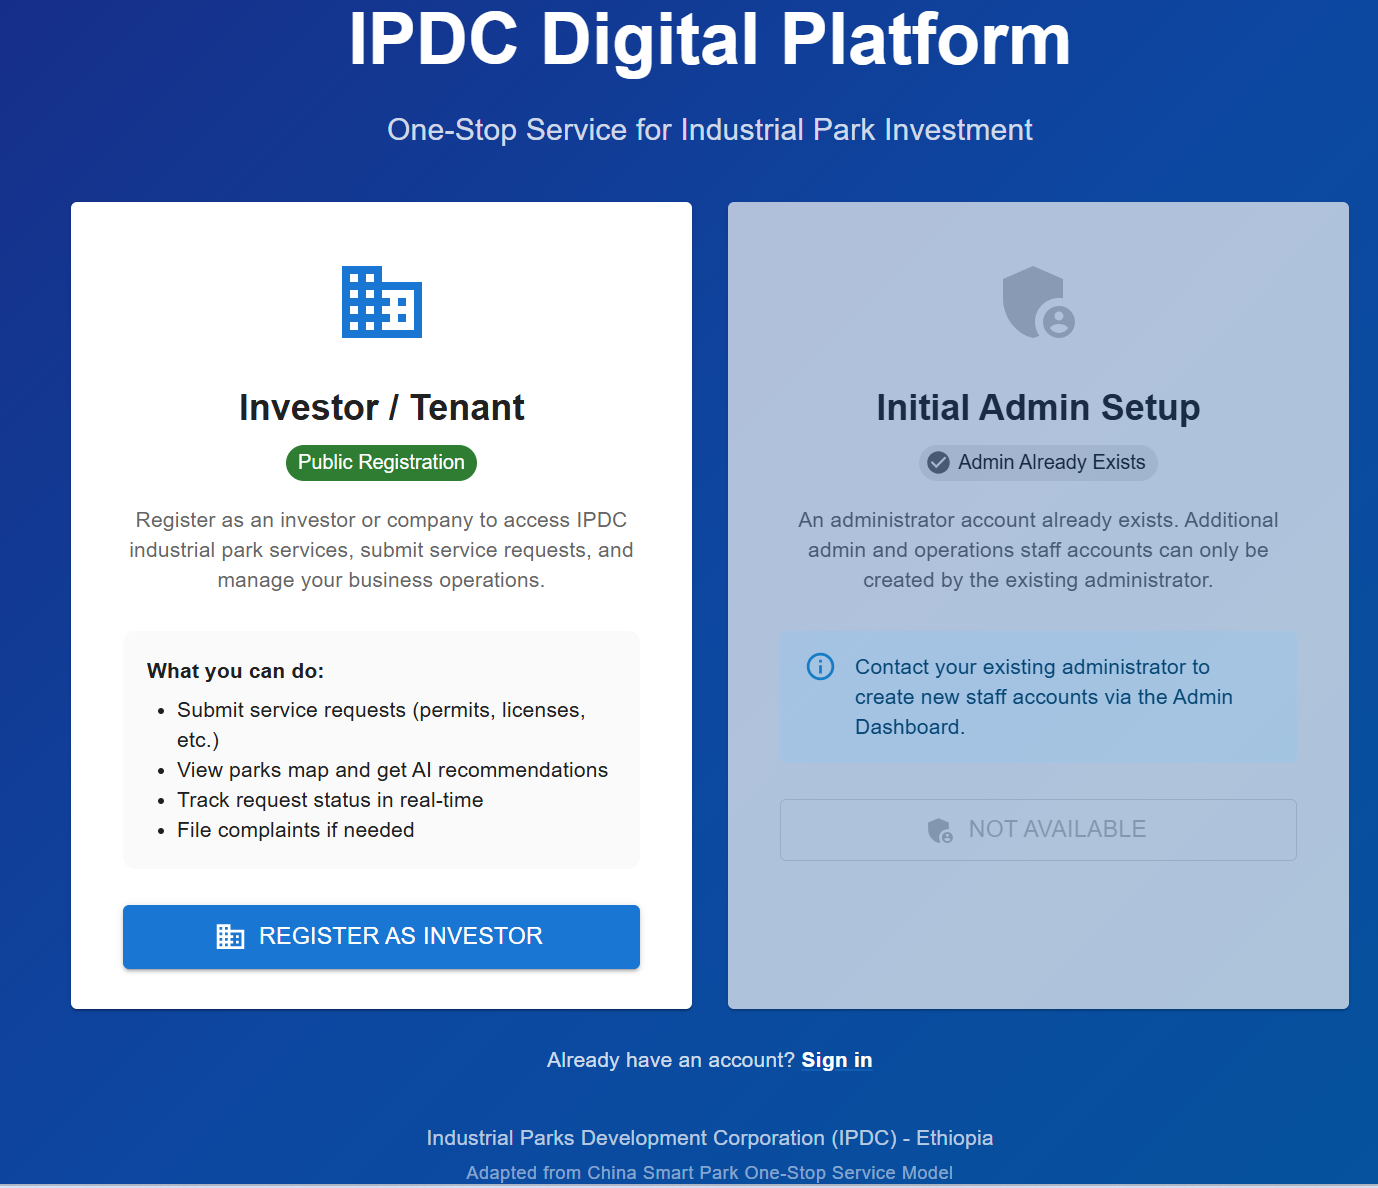
\includegraphics[width=\textwidth]{figures/fig_sign_up.png}
\end{minipage}
\caption[Authentication Interfaces]{Authentication Interfaces --- Sign-In (left) and Tenant Registration (right)}
\label{fig:auth-interfaces}
\end{figure}

\subsection{Service Request Management}

Service request management forms the backbone of the platform. The \texttt{CreateRequestForm} component (\texttt{src/components/tenant/}) uses React Hook Form for state management and Zod for schema validation. Requests can be categorized across multiple service types (maintenance, IT support, security, cleaning, waste management, and others), assigned one of four priority levels, given free-text descriptions, and accompanied by file attachments uploaded through the \texttt{FileUpload} component to Firebase Storage.

Each request follows a defined status progression: \texttt{pending} $\rightarrow$ \texttt{approved} $\rightarrow$ \texttt{in-progress} $\rightarrow$ \texttt{completed}. Administrators may also \texttt{reject} a request with a stated reason. Every status transition triggers a notification and updates the record in Firestore --- or in the local queue when offline. Figure~\ref{fig:tenant-workflow} shows the tenant dashboard alongside the service request creation form.

\begin{figure}[H]
\centering
\begin{minipage}[t]{0.48\textwidth}
\centering
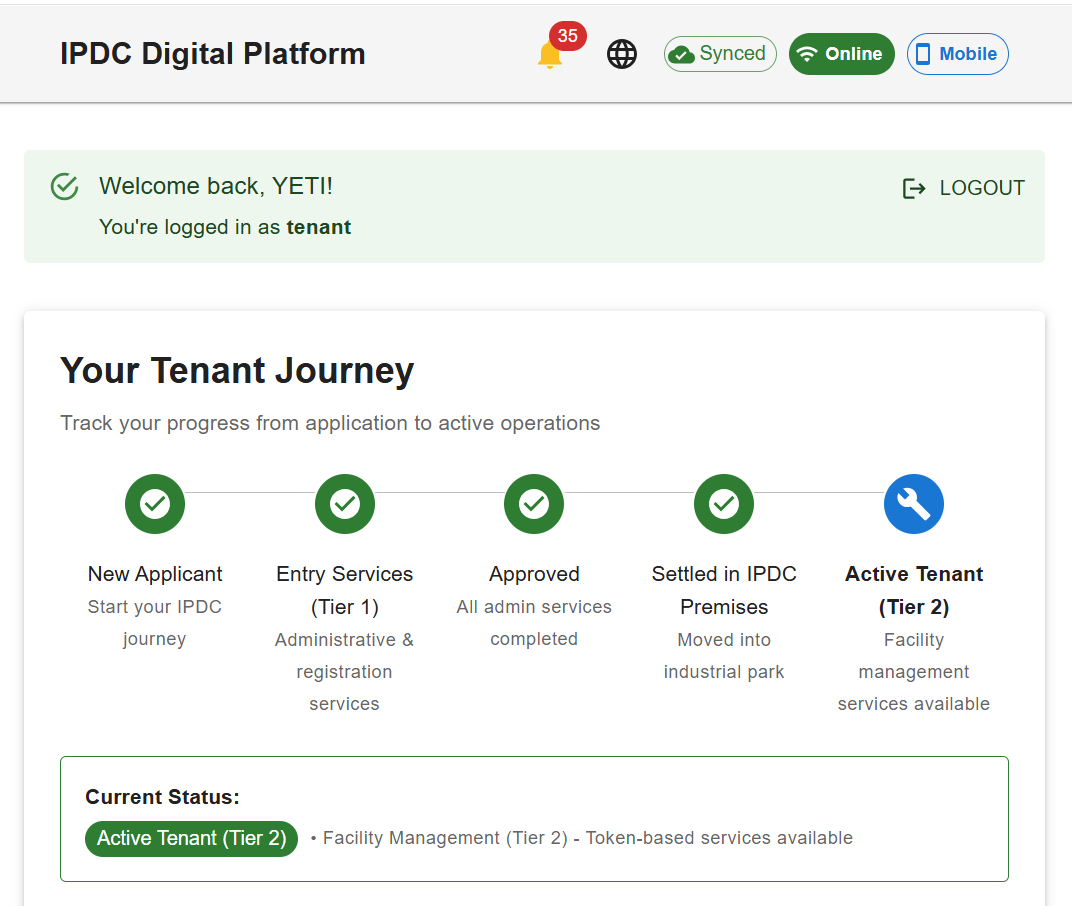
\includegraphics[width=\textwidth]{figures/fig_tenant_dashboard.png}
\end{minipage}
\hfill
\begin{minipage}[t]{0.48\textwidth}
\centering
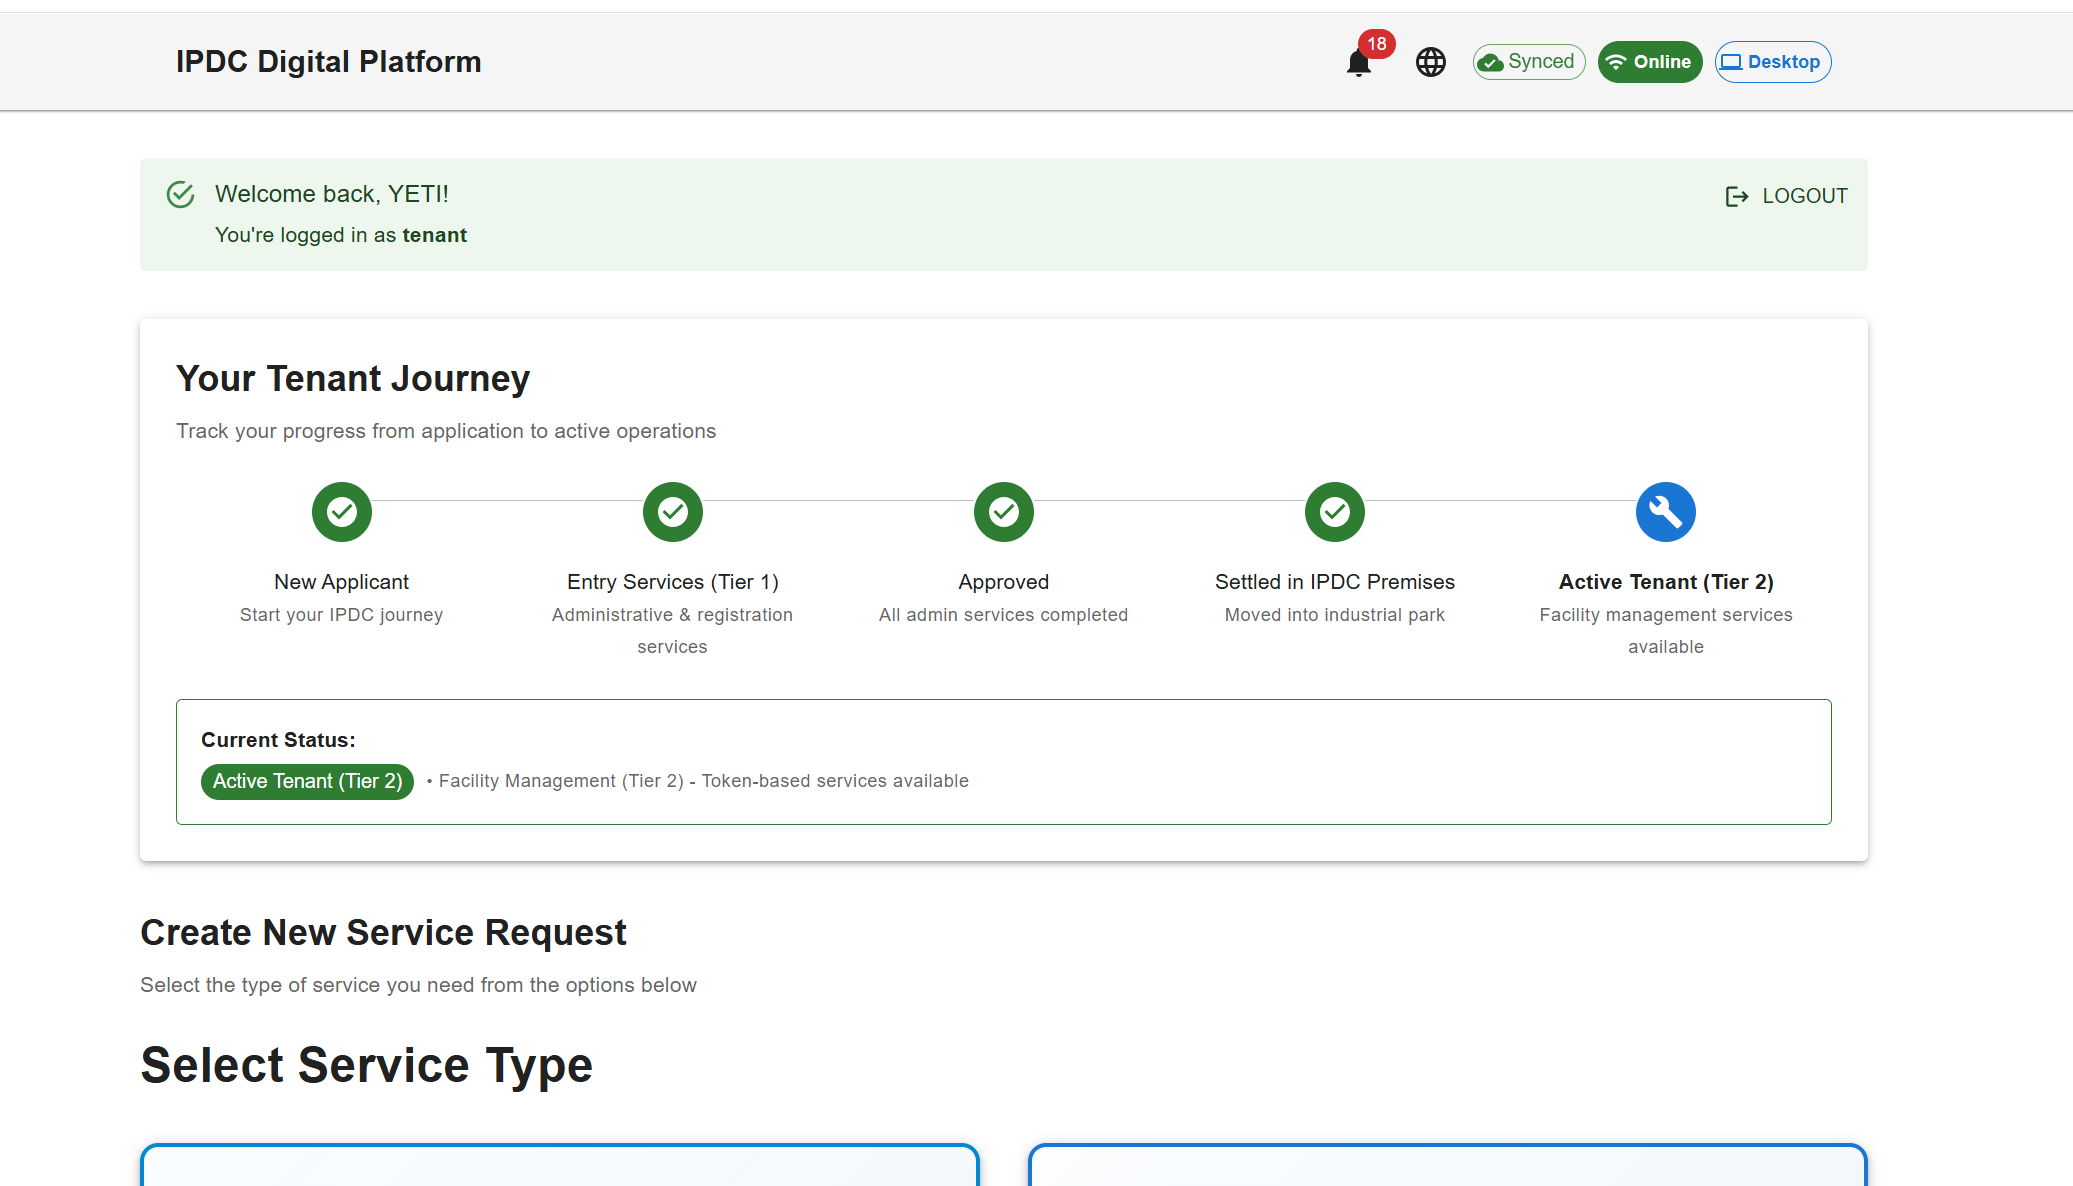
\includegraphics[width=\textwidth]{figures/fig_create_request.png}
\end{minipage}
\caption[Tenant Service Request Workflow]{Tenant Service Request Workflow --- Dashboard Overview (left) and Request Creation Form (right)}
\label{fig:tenant-workflow}
\end{figure}

\subsection{Digital Service Token System}

The token system provides an internal mechanism for tracking service fees without requiring an external payment gateway. Its implementation spans the \texttt{TokenDashboard} component and the \texttt{billingService} module.

\textbf{Token Tiers} reward engagement: basic through platinum (four tiers), each unlocking progressively larger discounts (0--20\%), higher monthly request limits, and priority support.

\textbf{Service Costs} vary by both service type and priority level. Table~\ref{tab:token-costs} shows the pricing matrix.

\begin{table}[H]
\centering
\caption{Service Token Pricing Matrix (tokens per request)}
\label{tab:token-costs}
\small
\begin{tabular}{lcccc}
\toprule
\textbf{Service Type} & \textbf{Low} & \textbf{Medium} & \textbf{High} & \textbf{Urgent} \\
\midrule
Maintenance & 50 & 80 & 120 & 150 \\
IT Support & 60 & 100 & 140 & 180 \\
Security & 40 & 65 & 95 & 120 \\
Cleaning & 25 & 45 & 65 & 80 \\
Waste Management & 35 & 60 & 85 & 110 \\
\bottomrule
\end{tabular}
\end{table}

A complete audit trail covers all transaction types (allocation, deduction, refund, bonus, penalty, purchase). Administrators credit tokens after confirming external payment receipt. Figure~\ref{fig:token-dashboard} shows the token dashboard interface.

\begin{figure}[H]
\centering

\includegraphics[width=0.75\textwidth]{figures/fig_token_dashboard.png}
\caption{Digital Service Token Dashboard}
\label{fig:token-dashboard}
\end{figure}

\subsection{AI Model Integration}

Three machine learning models are connected to the platform through a FastAPI backend. The frontend AI service module (\texttt{src/services/aiService.ts}) exposes typed interfaces for each model endpoint, with error handling and timeout management built in.

\textbf{Model 1 --- Service Classifier:} Trained on labeled service request data, this model sorts incoming requests into eleven service categories and assigns priority levels. Because the endpoint returns a confidence score, the interface presents predictions as suggestions that users can accept or override.

\textbf{Model 2 --- Predictive Maintenance:} This was the model stakeholders responded to most immediately during the usability evaluation --- the idea of warning operations staff before equipment fails, rather than after, resonated without any prompting. Given asset attributes, it produces a failure probability, risk level (low/medium/high), estimated days until failure, and a recommended maintenance action.

\textbf{Model 3 --- Park Recommendation:} Built to help prospective tenants choose a suitable industrial park, this model evaluates a tenant profile against park characteristics using a weighted scoring algorithm. Five dimensions --- industry alignment (30\%), capacity and availability (25\%), infrastructure match (20\%), cost efficiency (15\%), and location preference (10\%) --- produce ranked recommendations with detailed justifications.

All three models degrade gracefully: if the API is unreachable, the interface disables AI features without disrupting core service request and management workflows. Figure~\ref{fig:ai-interfaces} shows the service classifier and park recommendation interfaces; Figure~\ref{fig:predictive-views} presents the predictive maintenance module.

\begin{figure}[H]
\centering
\begin{minipage}[t]{0.48\textwidth}
\centering
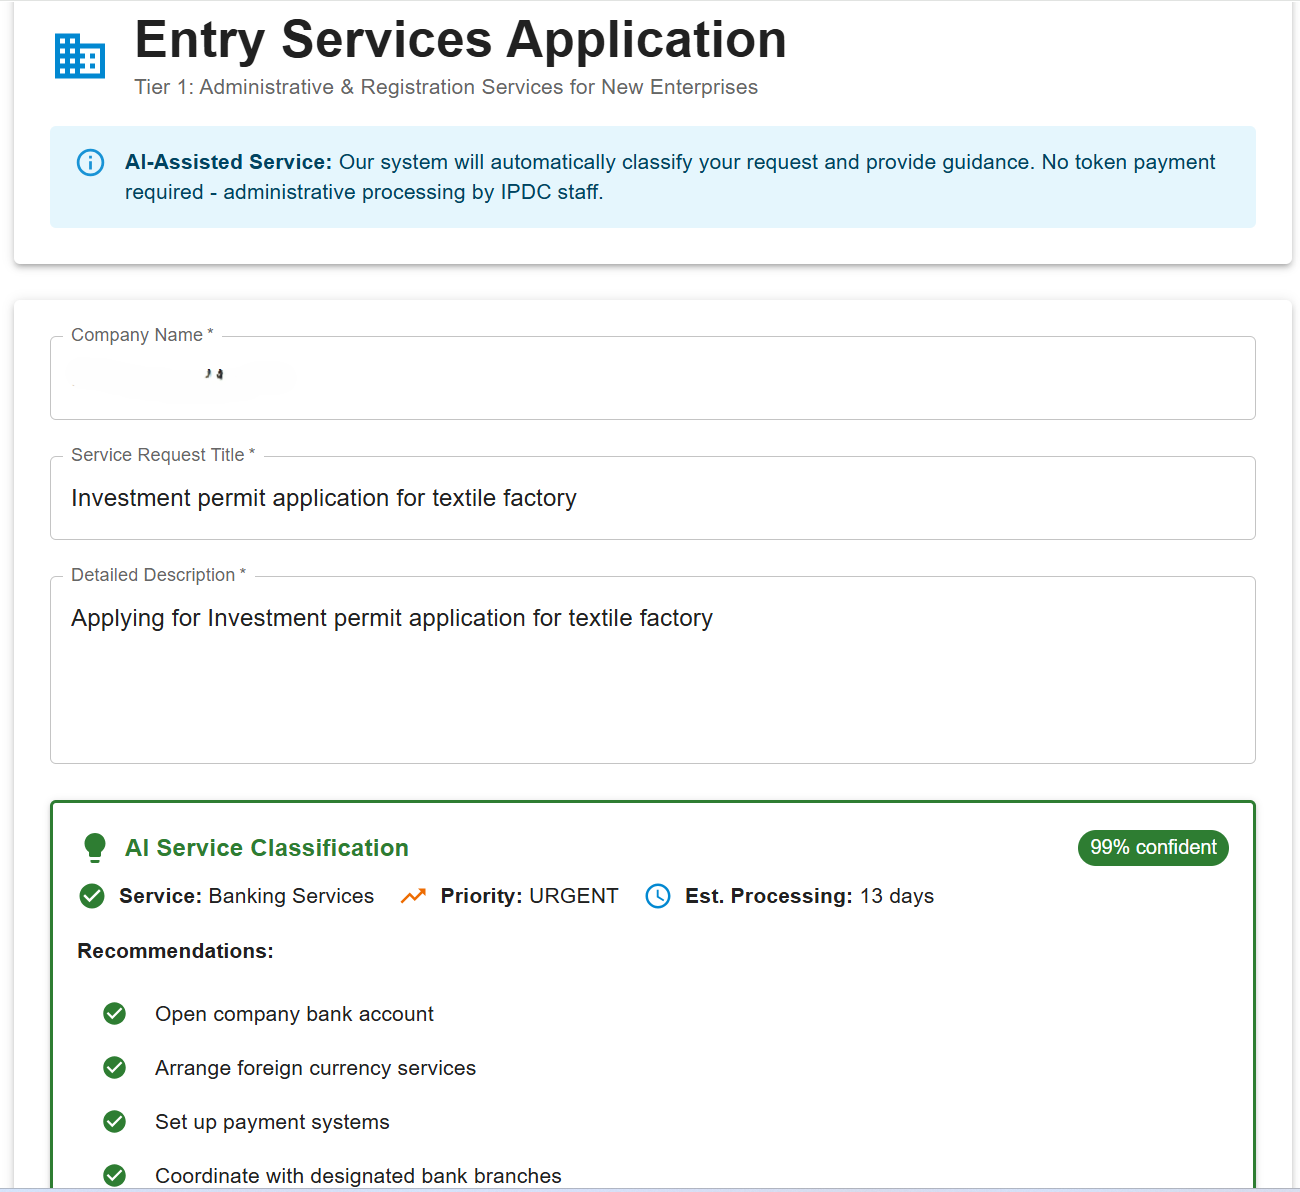
\includegraphics[width=\textwidth]{figures/fig_service_classifier.png}
\end{minipage}
\hfill
\begin{minipage}[t]{0.48\textwidth}
\centering
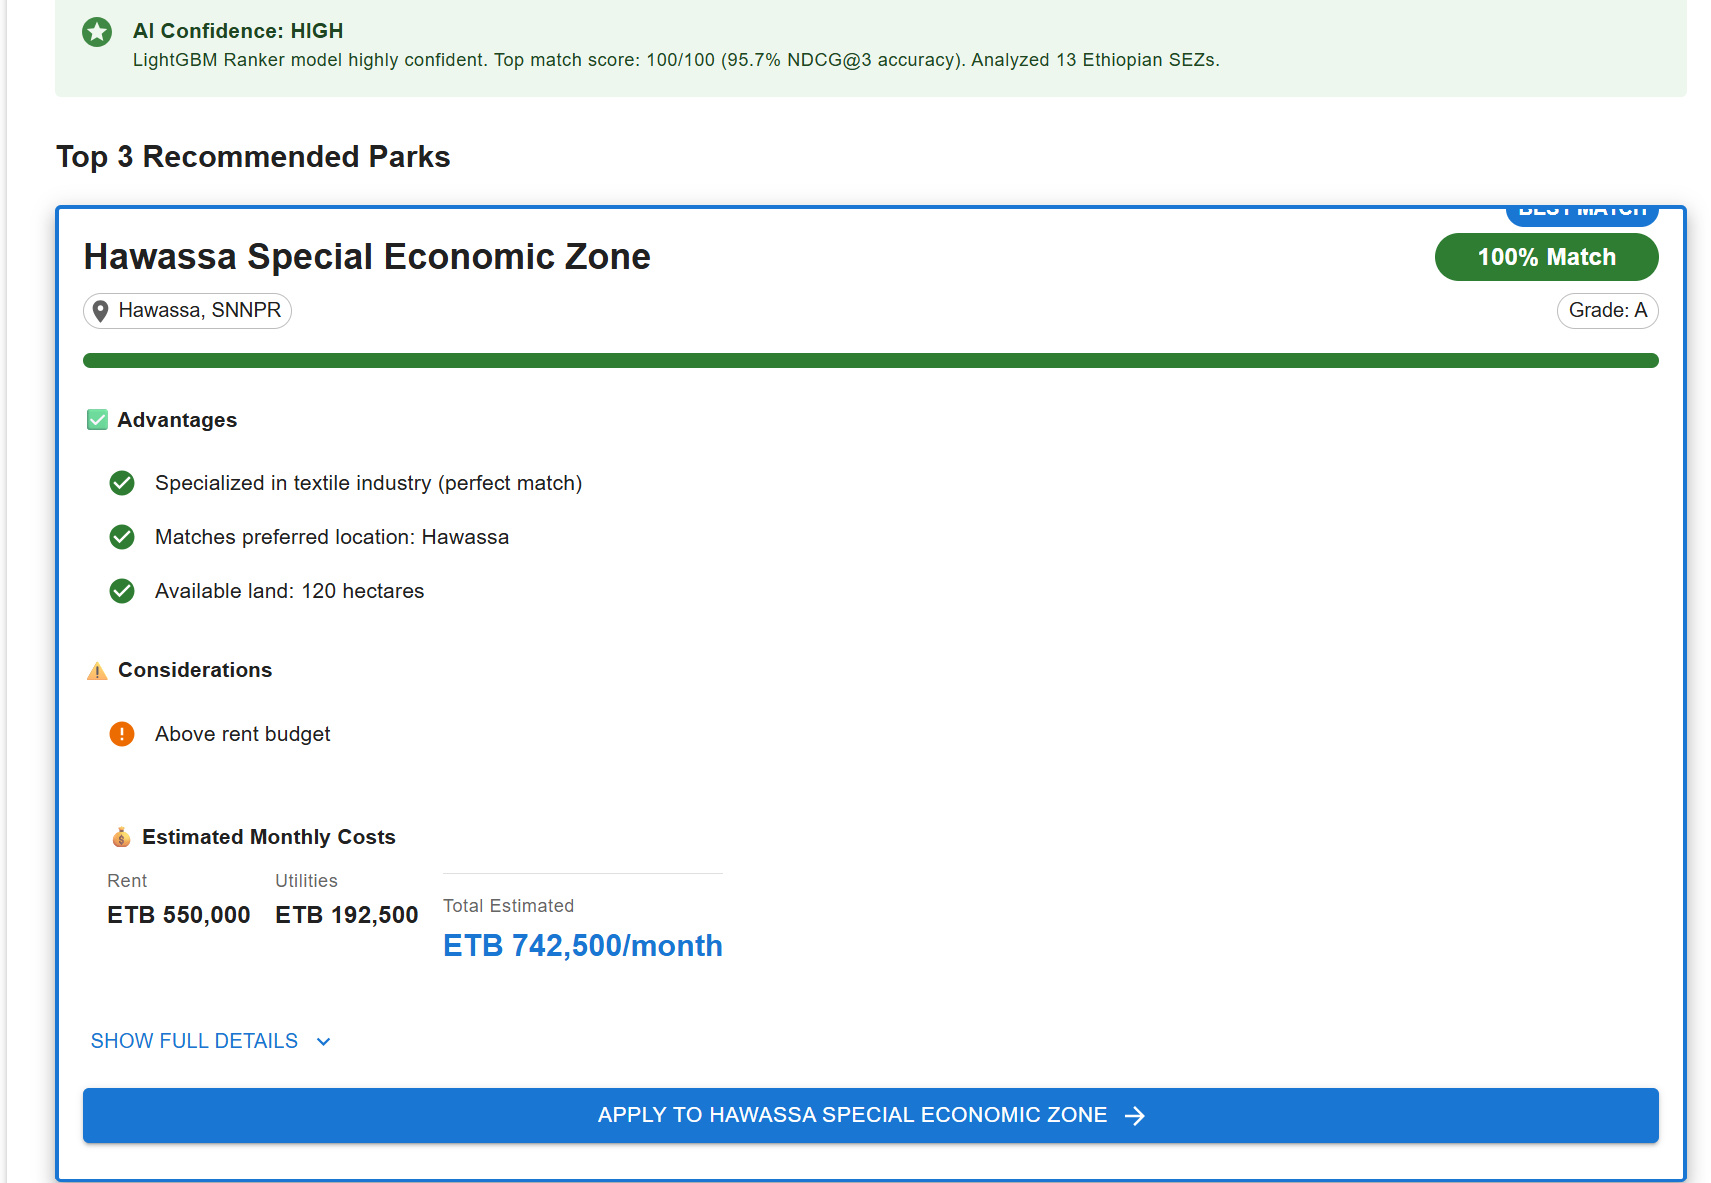
\includegraphics[width=\textwidth]{figures/fig_park_recommendation.png}
\end{minipage}
\caption[AI Model Interfaces]{AI Model Interfaces --- Service Classifier (left) and Park Recommendation (right)}
\label{fig:ai-interfaces}
\end{figure}

\begin{figure}[H]
\centering
\begin{minipage}[t]{0.48\textwidth}
\centering
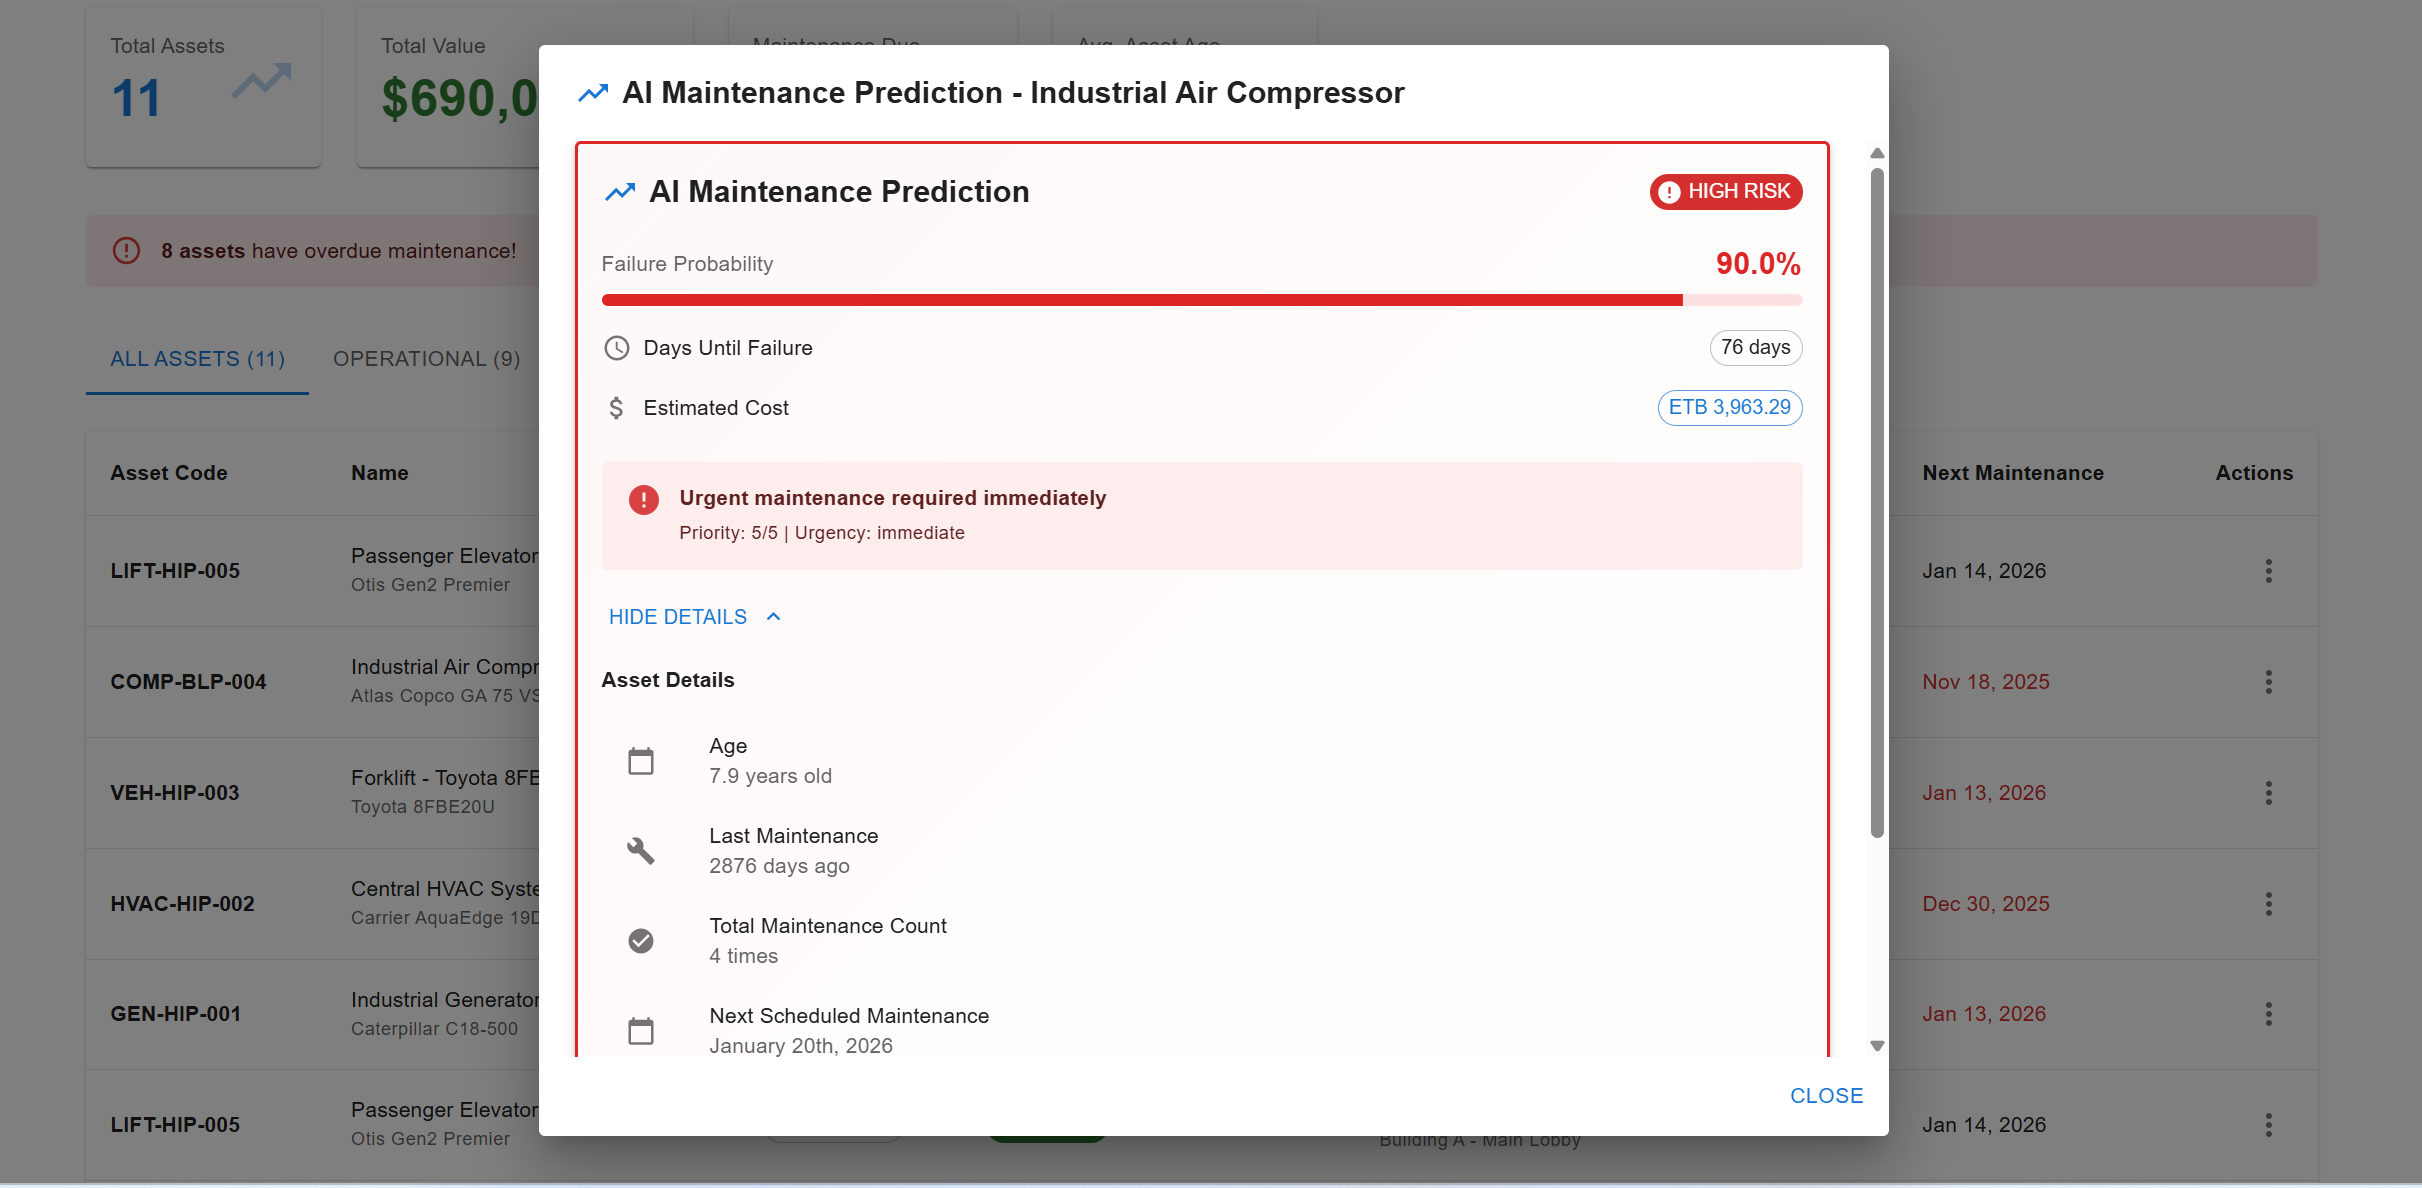
\includegraphics[width=\textwidth]{figures/fig_predictive_maintenance.png}
\end{minipage}
\hfill
\begin{minipage}[t]{0.48\textwidth}
\centering

\includegraphics[width=\textwidth]{figures/fig_predictive_maintenance_2.png}
\end{minipage}
\caption[Predictive Maintenance Views]{Predictive Maintenance Views --- Asset Overview (left) and Maintenance Detail (right)}
\label{fig:predictive-views}
\end{figure}

\subsection{Complaint Management System}

The complaint management module gives tenants a structured channel for raising issues with completed service requests. Nine complaint categories are available: service quality, incomplete work, delays, unprofessional conduct, billing dispute, facility issue, safety concern, communication gap, and other. Each complaint supports evidence uploads (images, documents, videos) and follows a resolution workflow: \texttt{pending} $\rightarrow$ \texttt{under-review} $\rightarrow$ \texttt{resolved} or \texttt{rejected}. Resolution actions range from full or partial token refund to service rework and compensation, with a 48-hour SLA target tracked for each complaint. Figure~\ref{fig:communication-interfaces} shows the complaint management and announcement interfaces.

\begin{figure}[H]
\centering
\begin{minipage}[t]{0.48\textwidth}
\centering
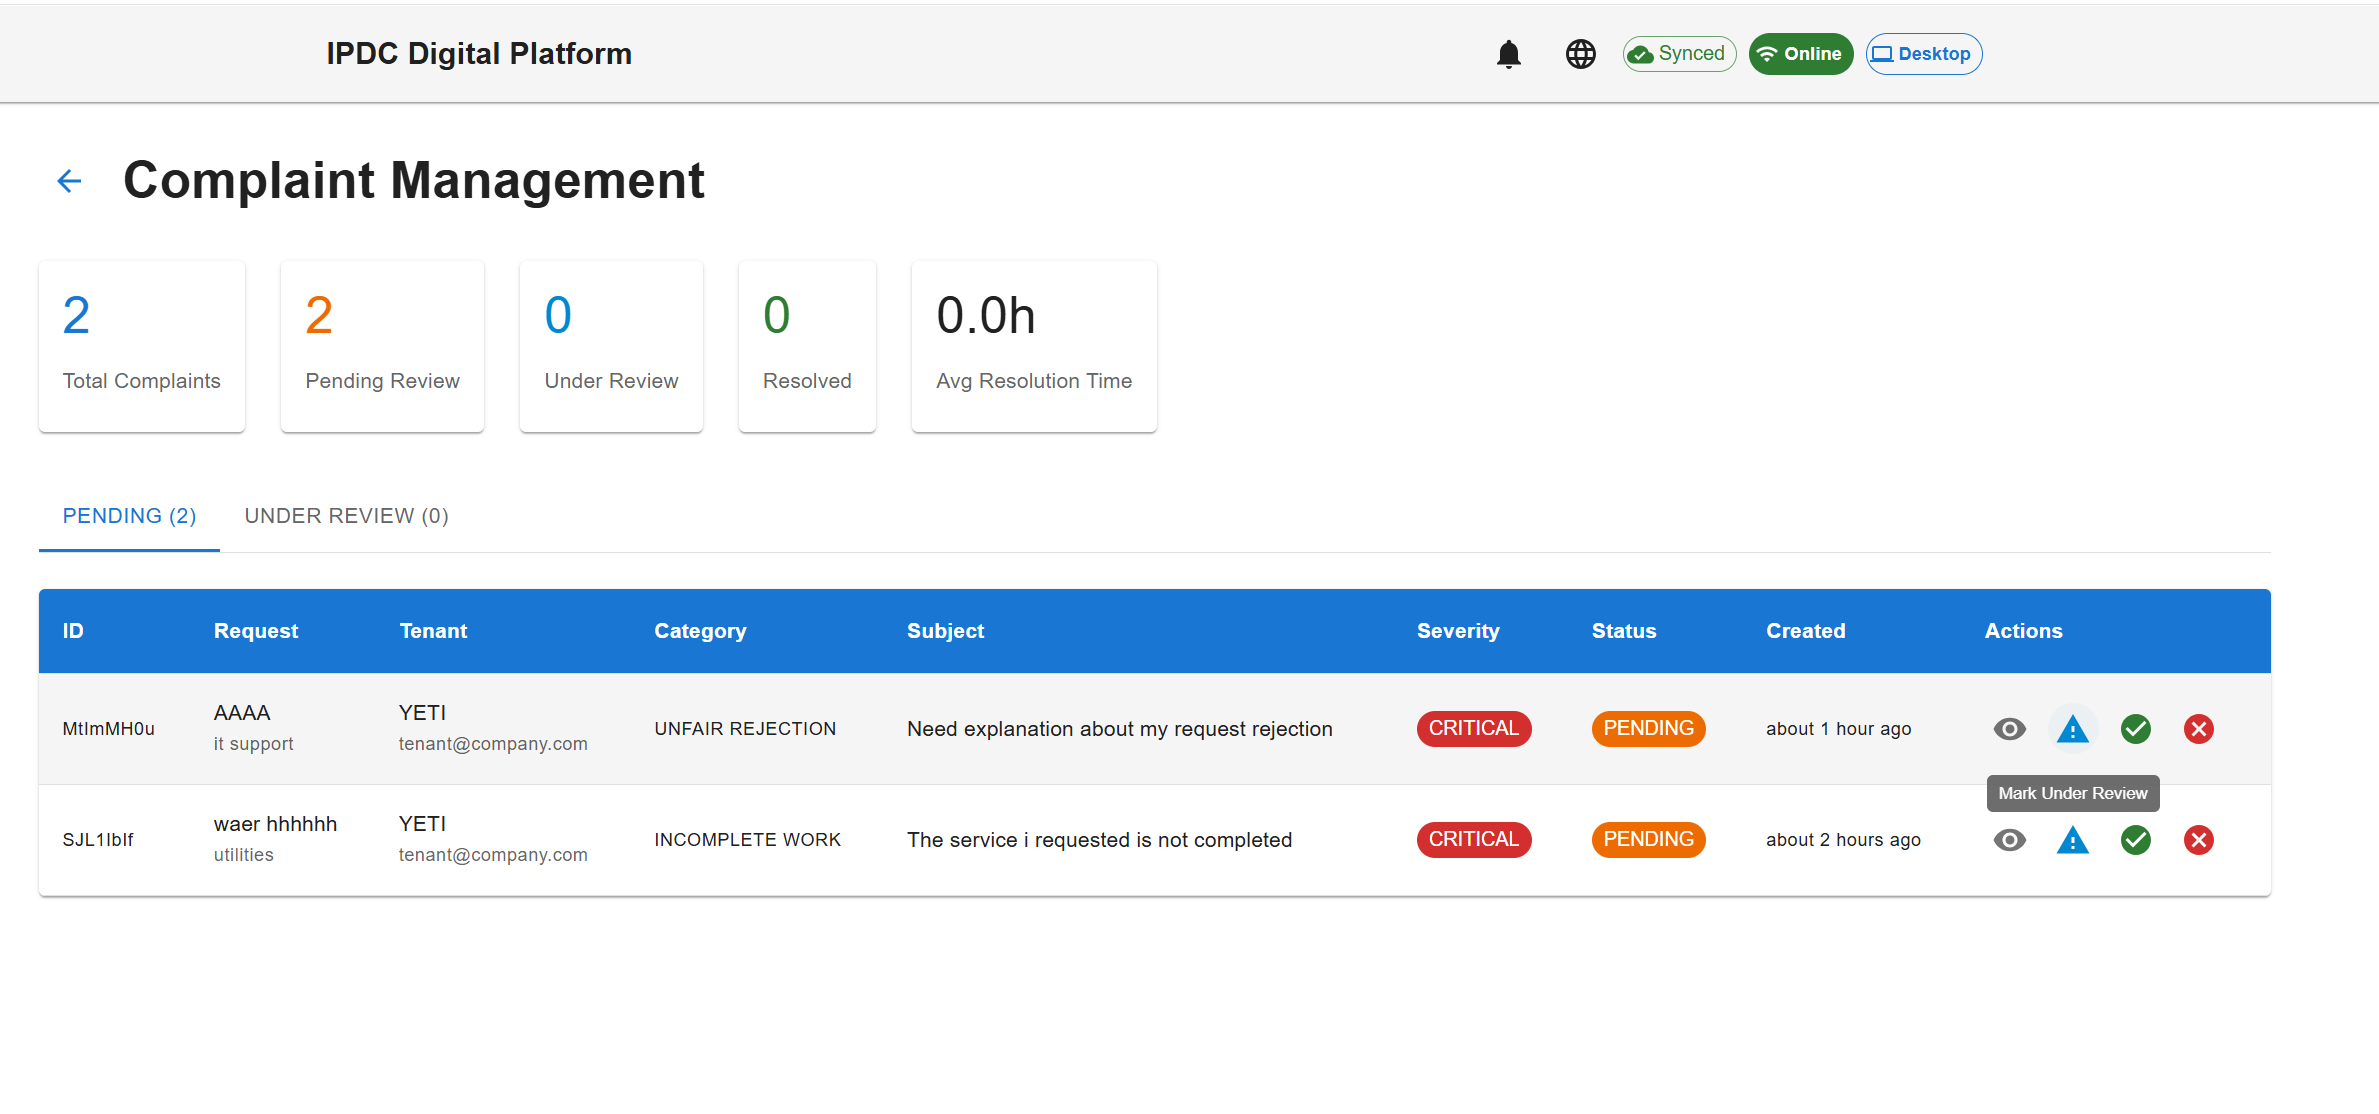
\includegraphics[width=\textwidth]{figures/fig_complaint_management.png}
\end{minipage}
\hfill
\begin{minipage}[t]{0.48\textwidth}
\centering

\includegraphics[width=\textwidth]{figures/fig_announcements.png}
\end{minipage}
\caption[Communication and Feedback Interfaces]{Communication and Feedback Interfaces --- Complaint Management (left) and Announcement System (right)}
\label{fig:communication-interfaces}
\end{figure}

\subsection{Announcement System}

The announcement module lets administrators create and distribute notices targeted at specific audience groups (all users, tenants only, operations only, or admin only). Each announcement carries a priority level, an optional expiration date, and an active/inactive toggle. The \texttt{AnnouncementBanner} component displays active announcements prominently across the interface, as shown in Figure~\ref{fig:communication-interfaces}.

\subsection{Interactive Park Map}

The park map module uses Leaflet and React-Leaflet to render an interactive geographic visualization of Ethiopian industrial parks. Clicking a marker opens a \texttt{ParkDetailsModal} displaying location details, available infrastructure, operational status, and tenant composition. Park coordinate data is stored in a static file within the application, so the map remains available during offline operation. Figure~\ref{fig:parks-map} shows the interface.

\begin{figure}[H]
\centering

\includegraphics[width=0.85\textwidth]{figures/fig_parks_map.png}
\caption{Interactive Industrial Parks Map}
\label{fig:parks-map}
\end{figure}

\subsection{Administrative Dashboard}

The admin dashboard (\texttt{src/pages/AdminDashboard.tsx}) is the central management interface. From here, administrators can view all service requests across the system, manage tenant accounts, create announcements, resolve complaints, oversee token and billing records, and manage park assets. Tabbed navigation organizes these functions; summary statistics and charts (powered by Recharts) provide at-a-glance operational visibility. Park operators have a dedicated dashboard for day-to-day service operations within their assigned park. Both are shown in Figure~\ref{fig:management-dashboards}.

\begin{figure}[H]
\centering
\begin{minipage}[t]{0.48\textwidth}
\centering
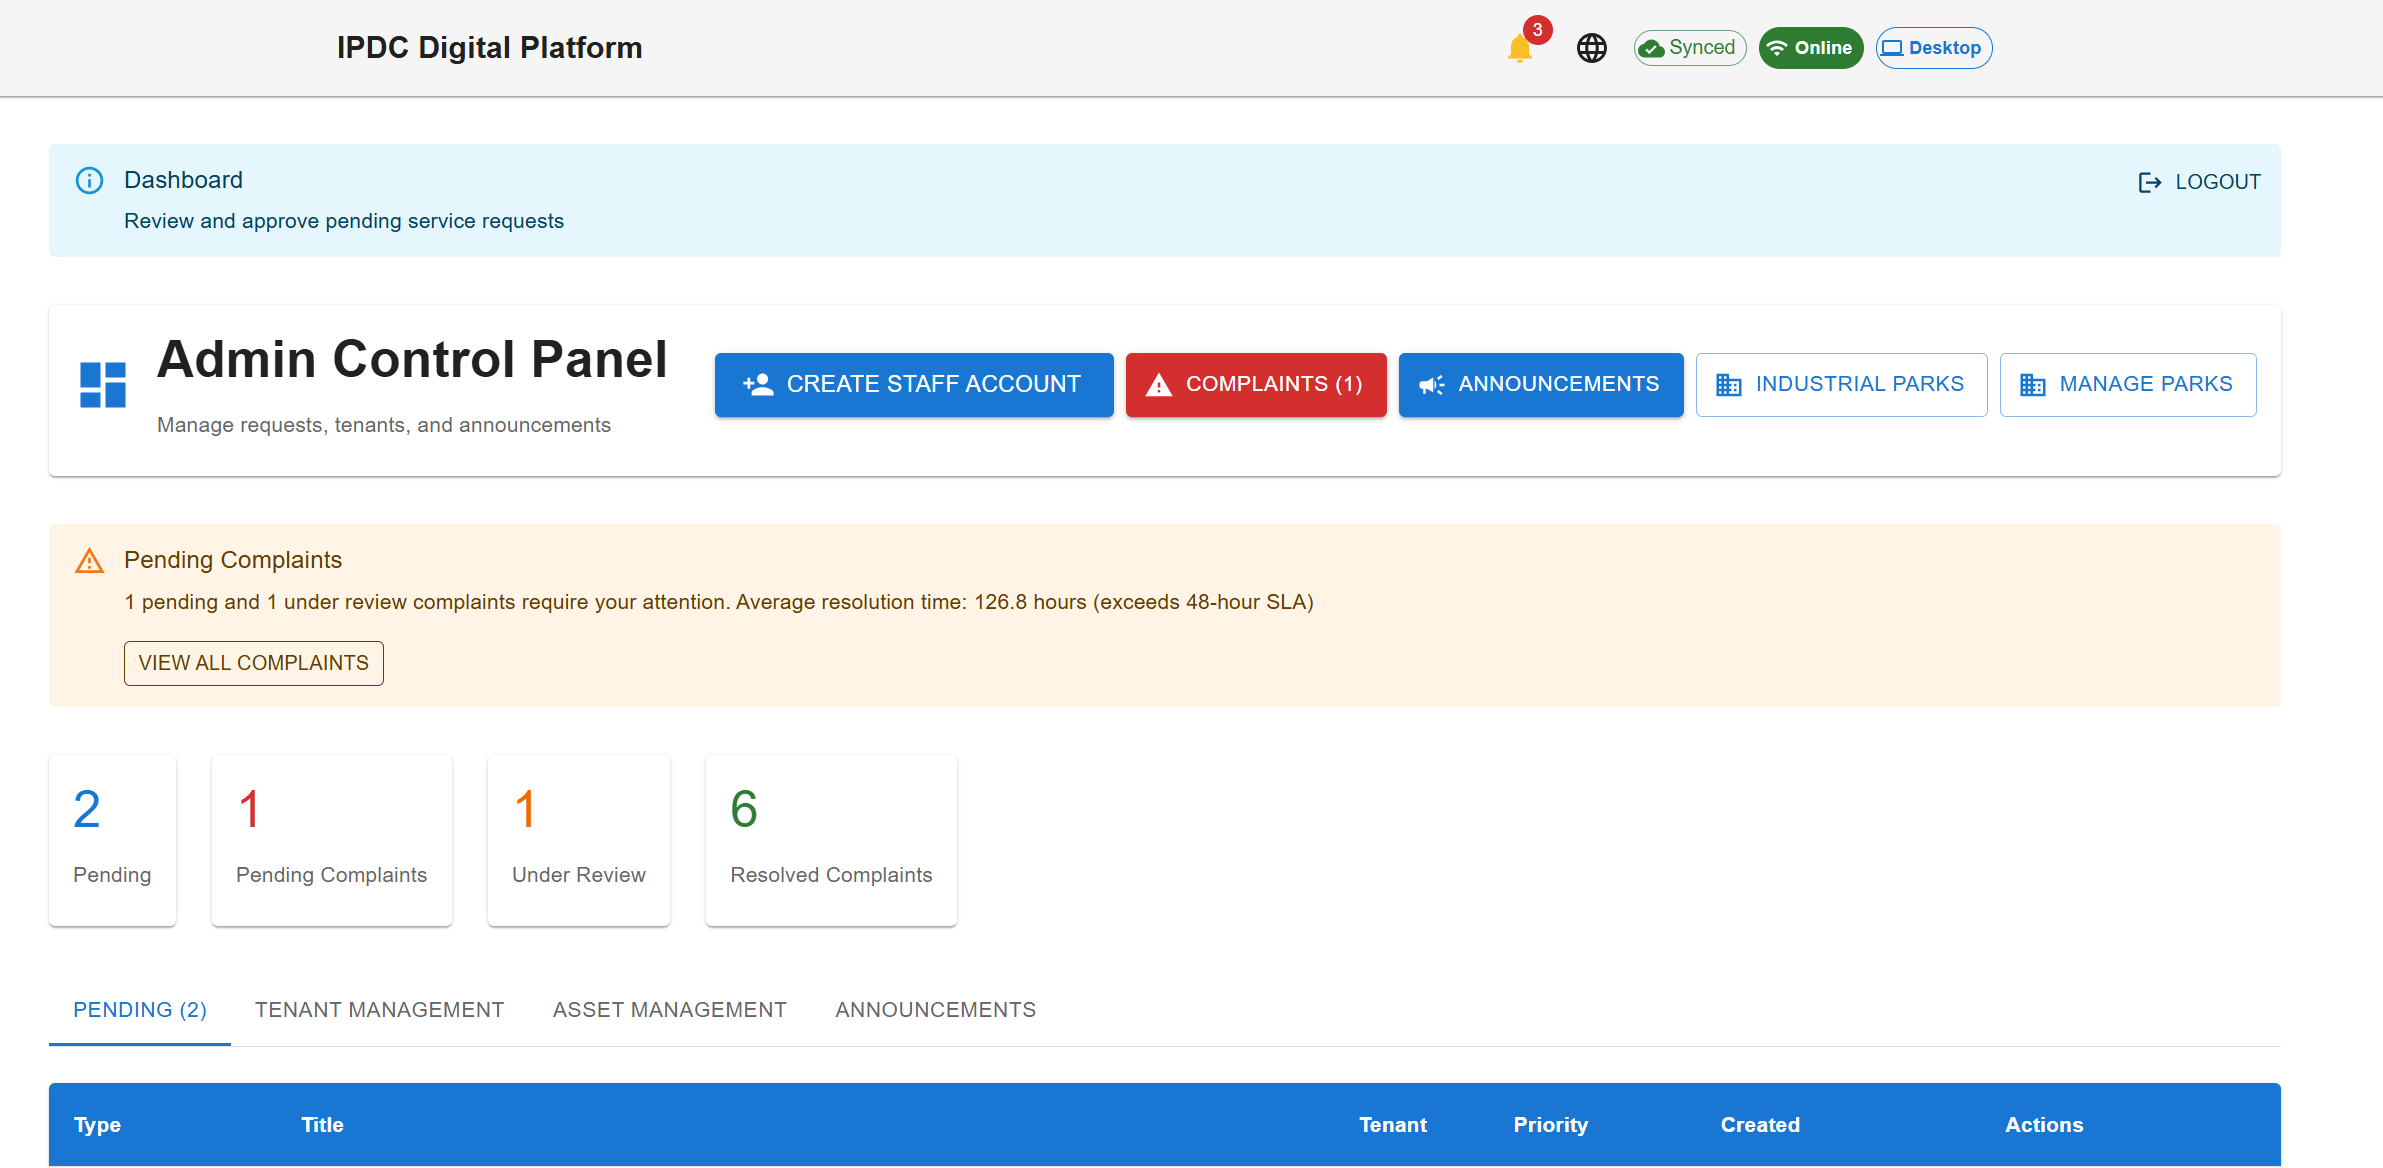
\includegraphics[width=\textwidth]{figures/fig_admin_dashboard.png}
\end{minipage}
\hfill
\begin{minipage}[t]{0.48\textwidth}
\centering
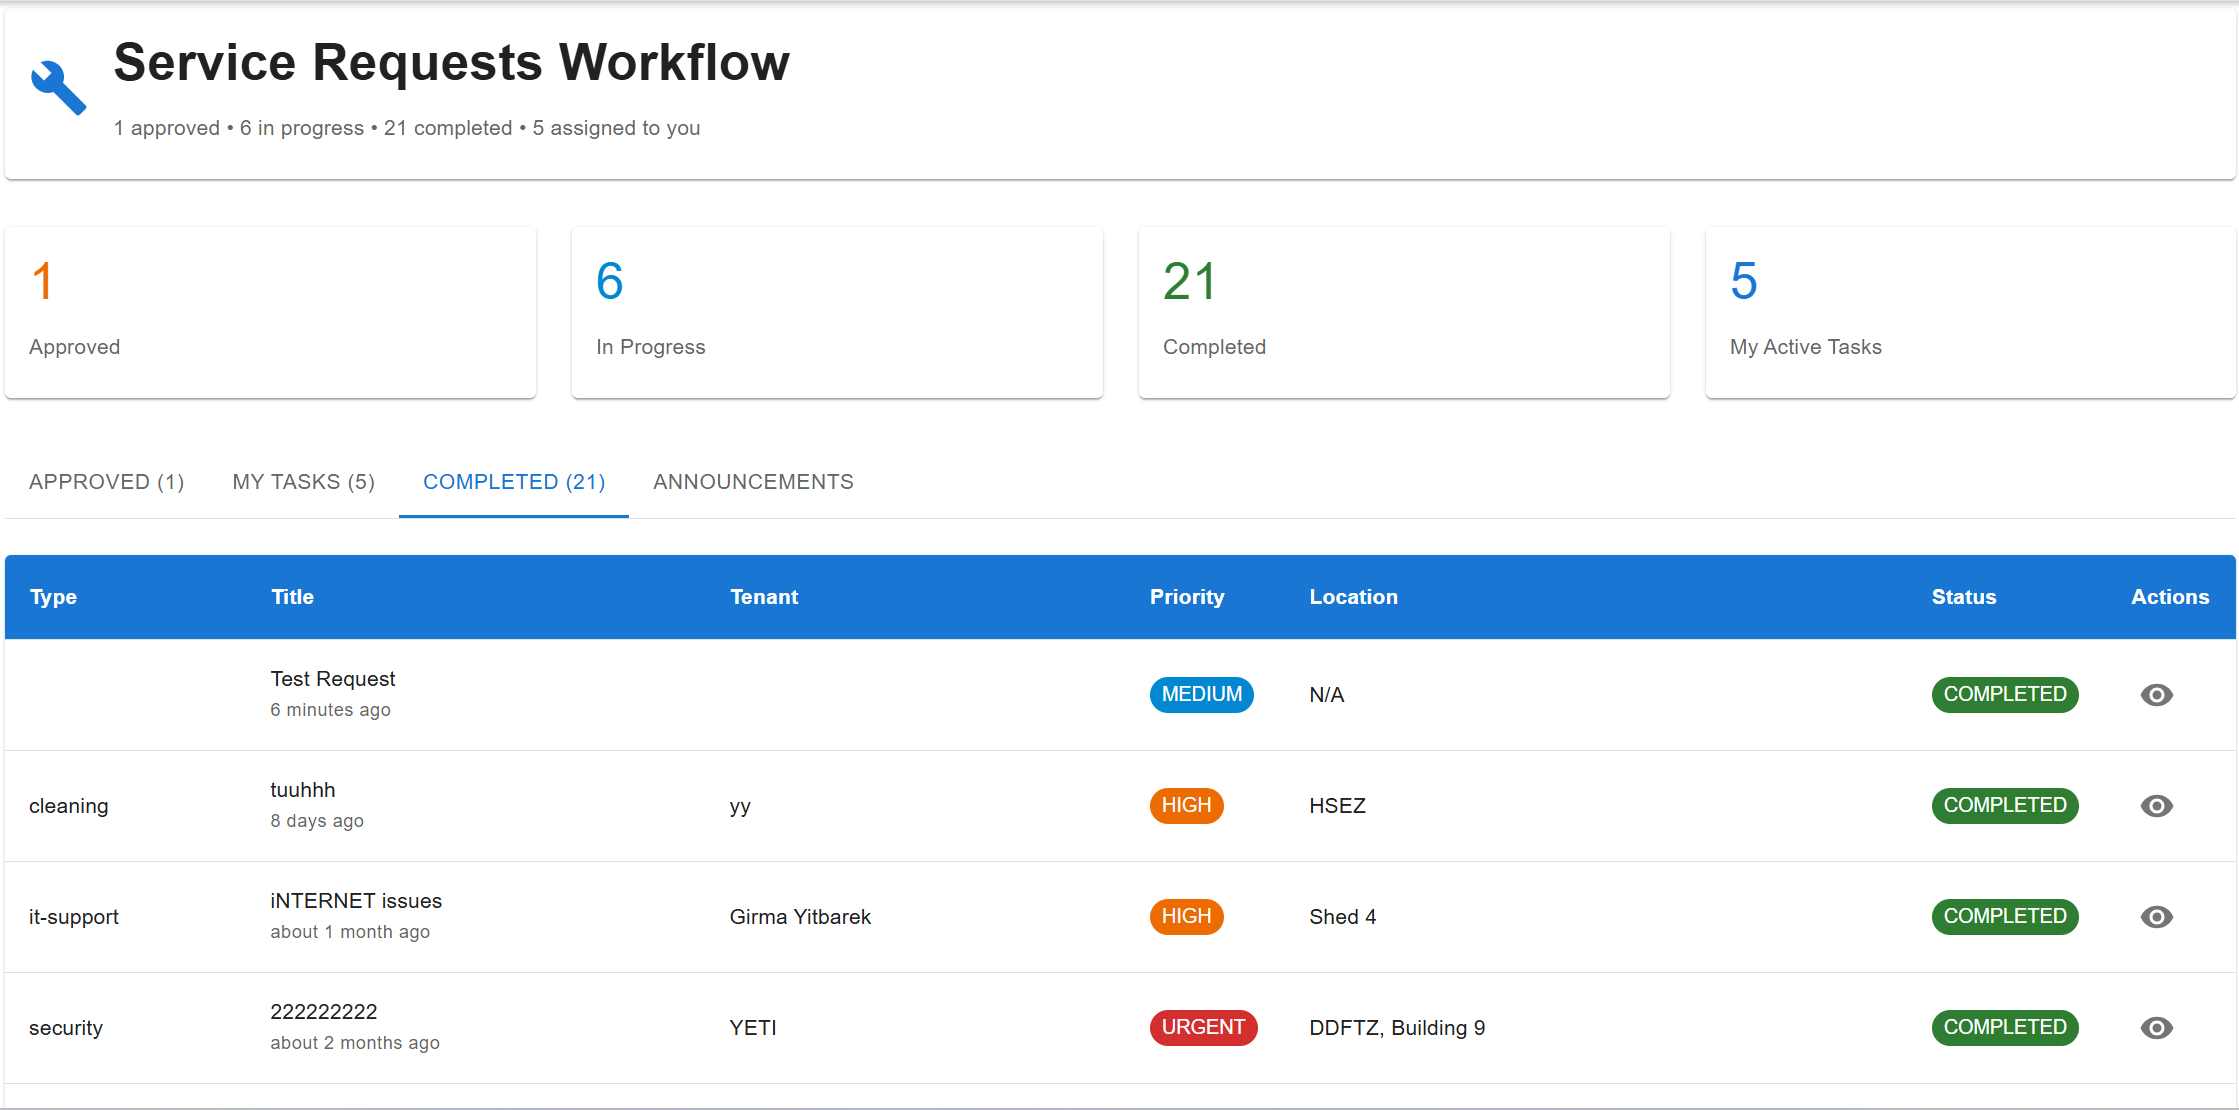
\includegraphics[width=\textwidth]{figures/fig_operators_dashboard.png}
\end{minipage}
\caption[Management Dashboard Interfaces]{Management Dashboard Interfaces --- Administrator (left) and Park Operators (right)}
\label{fig:management-dashboards}
\end{figure}

\section{AI Model Training and Evaluation}
\label{sec:ai-training}

This section documents how the three machine learning models were trained, what their data looks like, how they are structured, and how well they perform. All models were trained on synthetic datasets designed to reflect realistic IPDC operational patterns, with architectures informed by leading Chinese smart city systems --- Alibaba ET Industrial Brain, Tencent WeCity, and Huawei FusionPlant.

\subsection{Training Data}

Three domain-specific datasets were produced using the data synthesis pipeline (\texttt{ai-models/data/generate\_synthetic\_data.py}). Table~\ref{tab:training-data} summarizes their characteristics.

\begin{table}[H]
\centering
\caption{Training Dataset Characteristics}
\label{tab:training-data}
\small
\begin{tabular}{p{3.5cm}p{2cm}p{2cm}p{5cm}}
\toprule
\textbf{Dataset} & \textbf{Records} & \textbf{Features} & \textbf{Target Variables} \\
\midrule
Service Requests & 2,200 & 10 & Service type (11 classes), priority (4 classes), processing days (continuous) \\
Asset Maintenance & 500 & 14 & Failure flag (binary), days to failure (continuous), risk level (3 classes) \\
Park Placements & 10,400\textsuperscript{a} & 11 & Match score (relevance grade 0--4) \\
\bottomrule
\end{tabular}

\vspace{0.3cm}
\footnotesize
\textsuperscript{a} 800 tenant profiles $\times$ 13 industrial parks = 10,400 ranking pairs.
\end{table}

The service requests dataset includes text fields (title, description) processed through TF-IDF vectorization, alongside temporal metadata (hour of day, day of week) and text statistics (word count, character length). The asset maintenance dataset captures equipment attributes such as age, condition scores, maintenance history, and sensor readings (temperature, vibration level). The park placements dataset pairs every tenant profile with all 13 Ethiopian industrial parks in a learning-to-rank format, where the chosen park receives the highest relevance grade.

\subsection{Model 1: Smart Service Classifier}

\subsubsection{Architecture}

The service classifier is an XGBoost ensemble comprising three specialized sub-models. Text features are extracted using TF-IDF vectorization with a 1,500-term vocabulary (unigrams and bigrams, minimum document frequency of 2, maximum document frequency of 0.90). Four metadata features --- hour of day, day of week, text length, and word count --- are scaled with StandardScaler and concatenated with the TF-IDF vectors, yielding 1,504 input features per request.

\begin{table}[H]
\centering
\caption{Service Classifier Configuration and Results}
\label{tab:model1-config}
\label{tab:model1-results}
\small

\textbf{(a) Sub-Model Configurations}\\[0.3em]
\begin{tabular}{p{3.5cm}p{2.5cm}p{2cm}p{2cm}p{2cm}}
\toprule
\textbf{Sub-Model} & \textbf{Objective} & \textbf{Depth} & \textbf{LR} & \textbf{Trees} \\
\midrule
Category Classifier & Multi-class softmax & 6 & 0.1 & 100 \\
Priority Predictor & Multi-class softmax & 5 & 0.1 & 80 \\
Time Estimator & Squared error & 4 & 0.1 & 60 \\
\bottomrule
\end{tabular}

\vspace{0.5cm}
\textbf{(b) Evaluation Results}\\[0.3em]
\begin{tabular}{p{5cm}cc}
\toprule
\textbf{Metric} & \textbf{Value} & \textbf{Benchmark\textsuperscript{a}} \\
\midrule
Service Type Accuracy & 100\% & 85--92\% \\
Priority Classification Accuracy & 40\% & --- \\
Processing Time MAE & 2.63 days & $\pm$3 days \\
Processing Time $R^{2}$ & 0.577 & --- \\
Average Confidence Score & 0.95 & --- \\
\bottomrule
\end{tabular}

\vspace{0.3cm}
\footnotesize
\textsuperscript{a} Alibaba ET Industrial Brain benchmark on similar classification tasks.
\end{table}

The training data was split into 70\% training (1,386 samples), 15\% validation (297 samples), and 15\% test (297 samples).

Category classification reaches 100\% on the synthetic set --- the eleven IPDC service types have distinct vocabulary patterns, making separation straightforward. The priority predictor's 40\% accuracy reflects the subjectivity of human judgment, not a shortcoming of the model. The time estimator's 2.63-day MAE offers tenants useful planning estimates. Figure~\ref{fig:model1-eval} presents the confusion matrix for service type classification and the scatter plot of predicted versus actual processing days.

\begin{figure}[H]
\centering
\begin{minipage}[t]{0.48\textwidth}
\centering
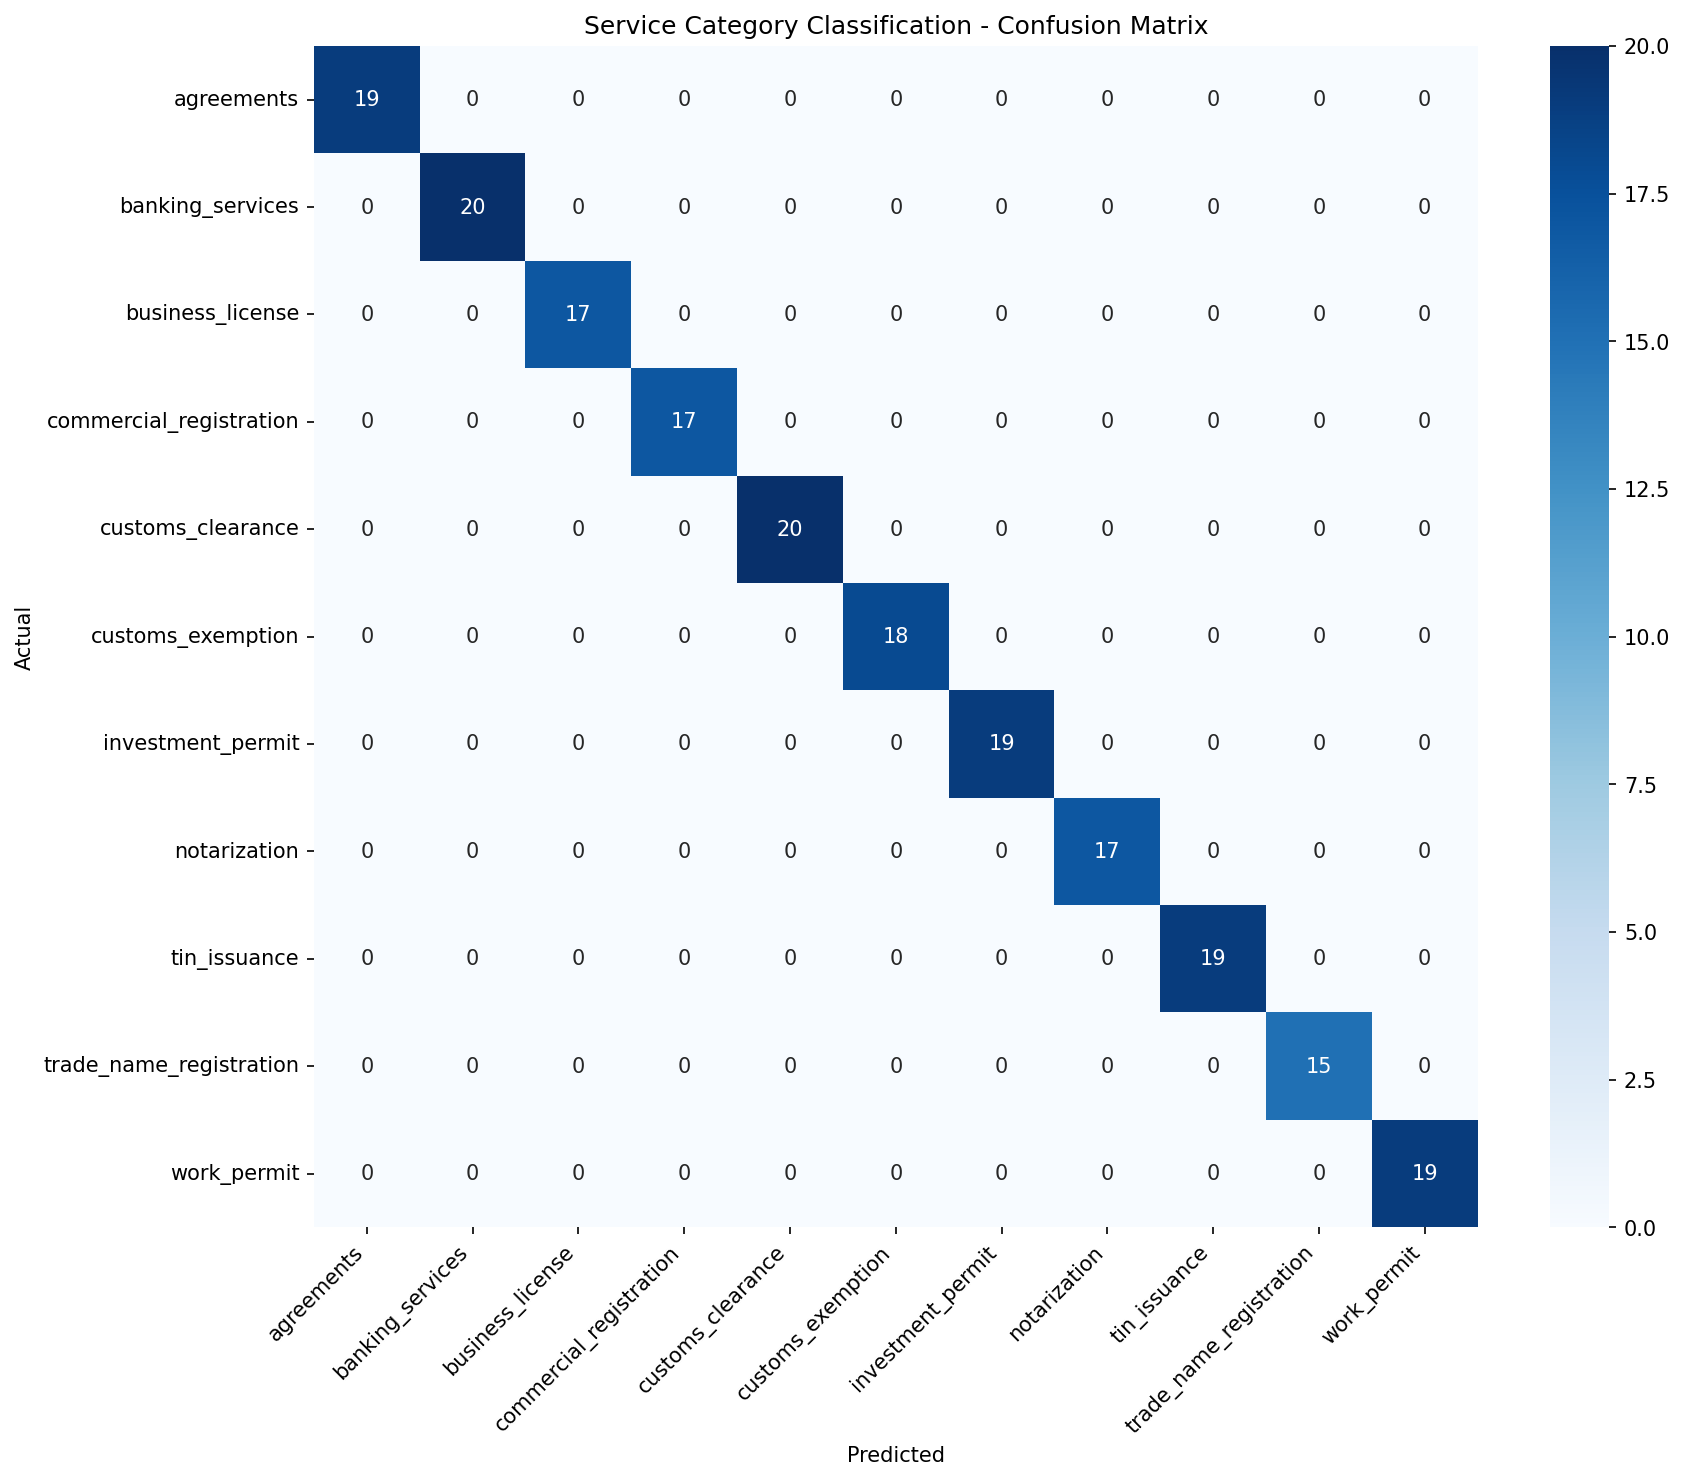
\includegraphics[width=\textwidth]{figures/model1_confusion_matrix_category.png}
\end{minipage}
\hfill
\begin{minipage}[t]{0.48\textwidth}
\centering
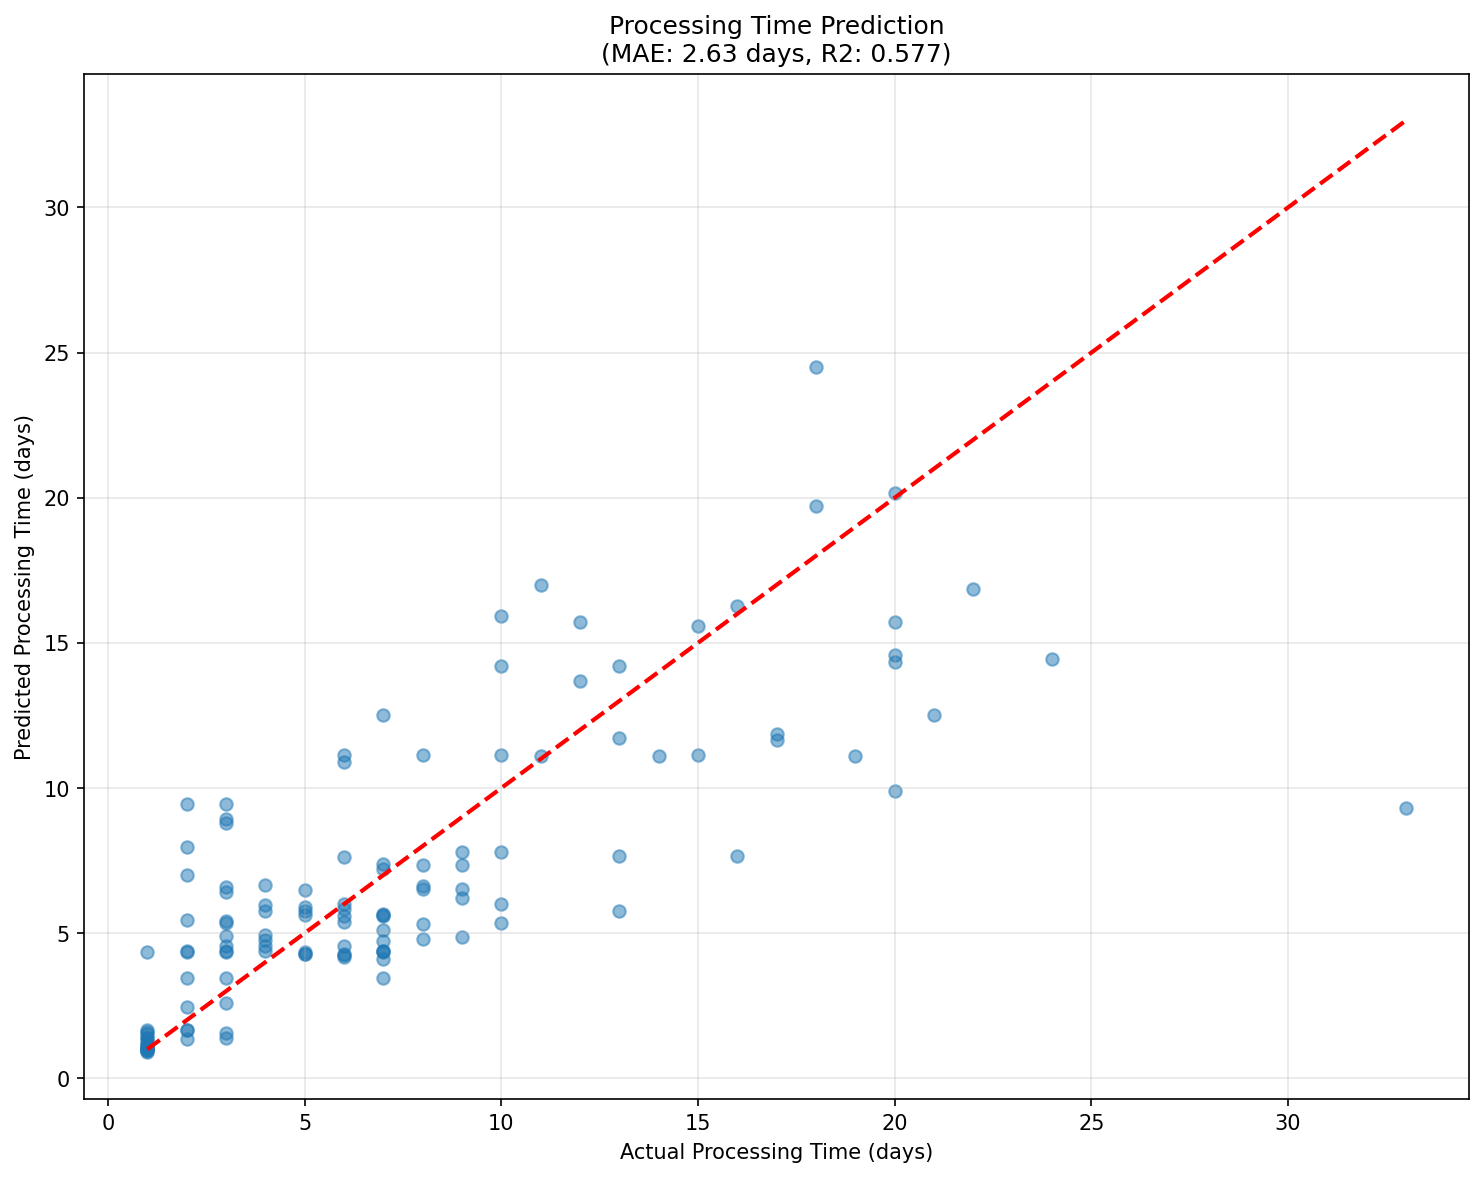
\includegraphics[width=\textwidth]{figures/model1_time_prediction_scatter.png}
\end{minipage}
\caption[Service Classifier Evaluation (Model 1)]{Service Classifier Evaluation (Model 1) --- Confusion Matrix (left) and Processing Time Prediction (right)}
\label{fig:model1-eval}
\end{figure}

\subsection{Model 2: Predictive Maintenance System}

\subsubsection{Architecture}

The predictive maintenance system combines two algorithms in a dual-algorithm ensemble: Random Forest for classification and Gradient Boosting for regression. Fourteen engineered features are derived from raw asset attributes, including age in days, days since last maintenance, cumulative maintenance count, operating hours, historical failure count, sensor readings (temperature, vibration level), and a composite condition score:

\begin{equation}
\text{Condition Score} = \frac{\text{age\_months}}{120} \times 30 + \frac{\text{days\_since\_maint}}{365} \times 30 + \text{failures} \times 10 + \frac{\text{hours}}{20000} \times 10
\label{eq:condition-score}
\end{equation}

Categorical features (asset category, status, condition level) are encoded with LabelEncoder; all features are normalized using StandardScaler.

\begin{table}[H]
\centering
\caption{Predictive Maintenance Configuration and Results}
\label{tab:model2-config}
\label{tab:model2-results}
\small

\textbf{(a) Sub-Model Configurations}\\[0.3em]
\begin{tabular}{p{3.5cm}p{3cm}p{2cm}p{2cm}p{2cm}}
\toprule
\textbf{Sub-Model} & \textbf{Algorithm} & \textbf{Depth} & \textbf{Trees} & \textbf{Min Leaf} \\
\midrule
Failure Predictor & Random Forest & 10 & 100 & 2 \\
Days-to-Failure & Gradient Boosting & 5 & 100 & --- \\
Risk Classifier & Random Forest & 10 & 100 & 2 \\
\bottomrule
\end{tabular}

\vspace{0.5cm}
\textbf{(b) Evaluation Results}\\[0.3em]
\begin{tabular}{p{5cm}cc}
\toprule
\textbf{Metric} & \textbf{Value} & \textbf{Benchmark\textsuperscript{a}} \\
\midrule
Failure Prediction Accuracy & 100\% & 80--88\% \\
Days Until Failure MAE & 0.014 days & --- \\
Days Until Failure $R^{2}$ & 0.9989 & --- \\
Risk Classification Accuracy & 99\% & --- \\
\bottomrule
\end{tabular}

\vspace{0.3cm}
\footnotesize
\textsuperscript{a} Huawei FusionPlant IoT predictive maintenance benchmark.
\end{table}

The training data was split into 70\% training (350 samples), 15\% validation (75 samples), and 15\% test (75 samples).

The near-perfect regression performance ($R^{2} = 0.9989$) reflects the tight relationship between the engineered features and failure timing in the synthetic dataset. The risk classifier reaches 99\% accuracy across low, medium, and high risk levels. Figure~\ref{fig:model2-eval} shows the risk classification confusion matrix and the scatter plot of predicted versus actual days to failure; Figure~\ref{fig:feature-importance-maintenance} displays the feature importance ranking.

\begin{figure}[H]
\centering
\begin{minipage}[t]{0.48\textwidth}
\centering
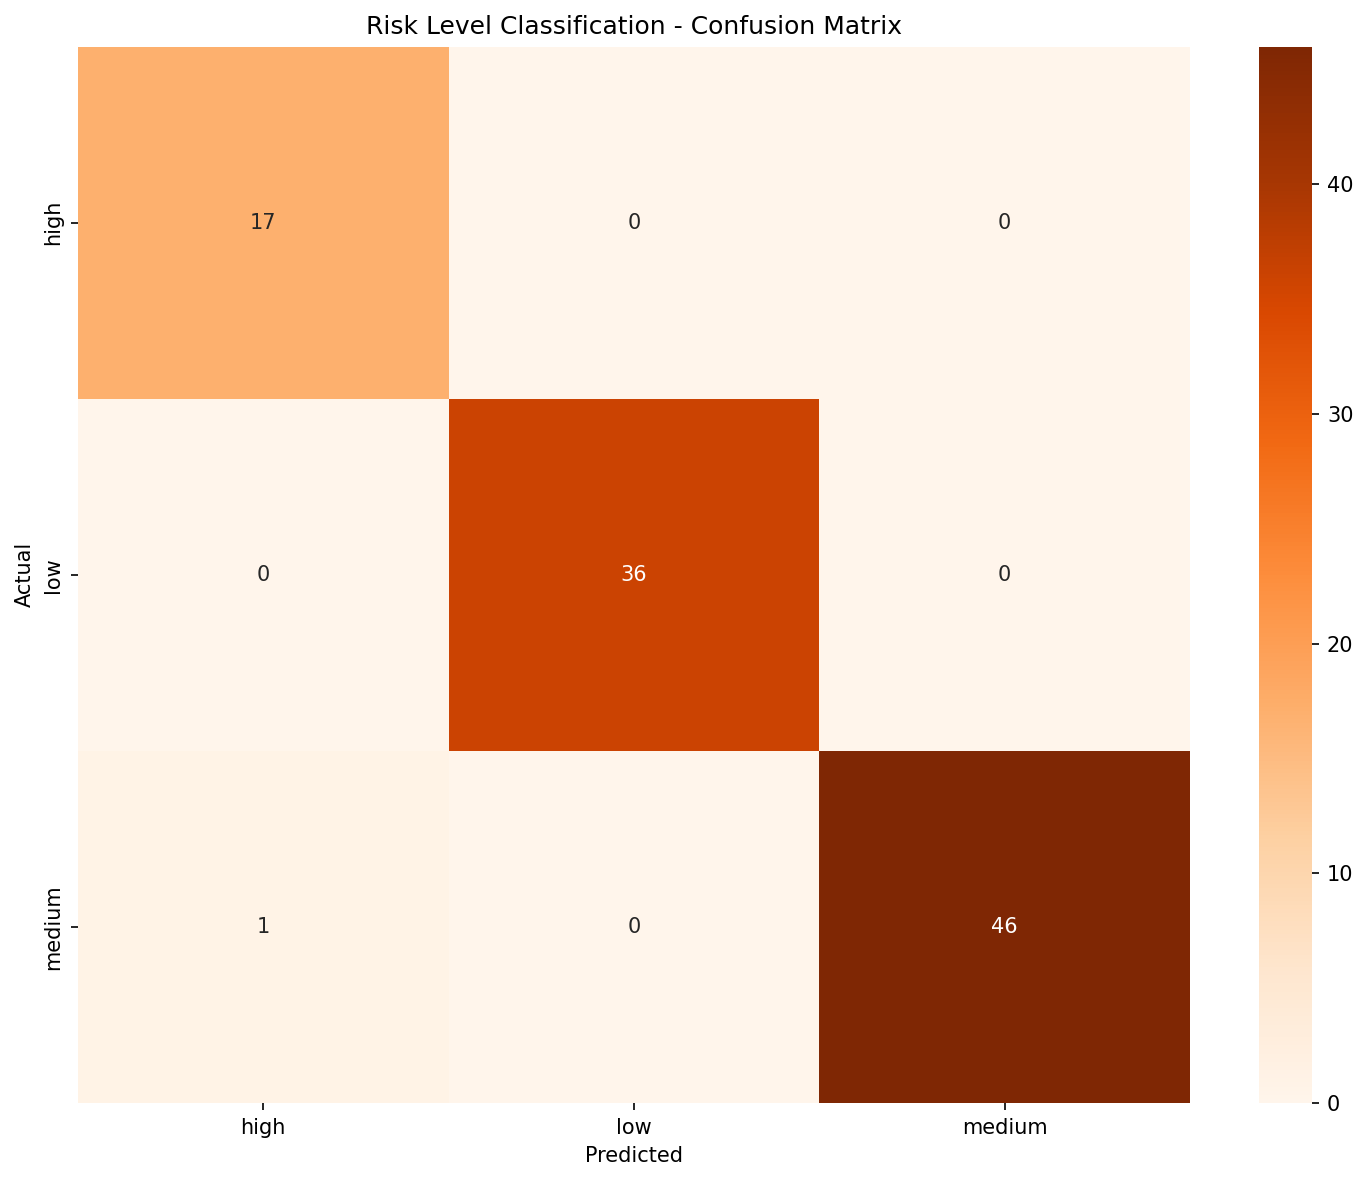
\includegraphics[width=\textwidth]{figures/model2_confusion_matrix_risk.png}
\end{minipage}
\hfill
\begin{minipage}[t]{0.48\textwidth}
\centering
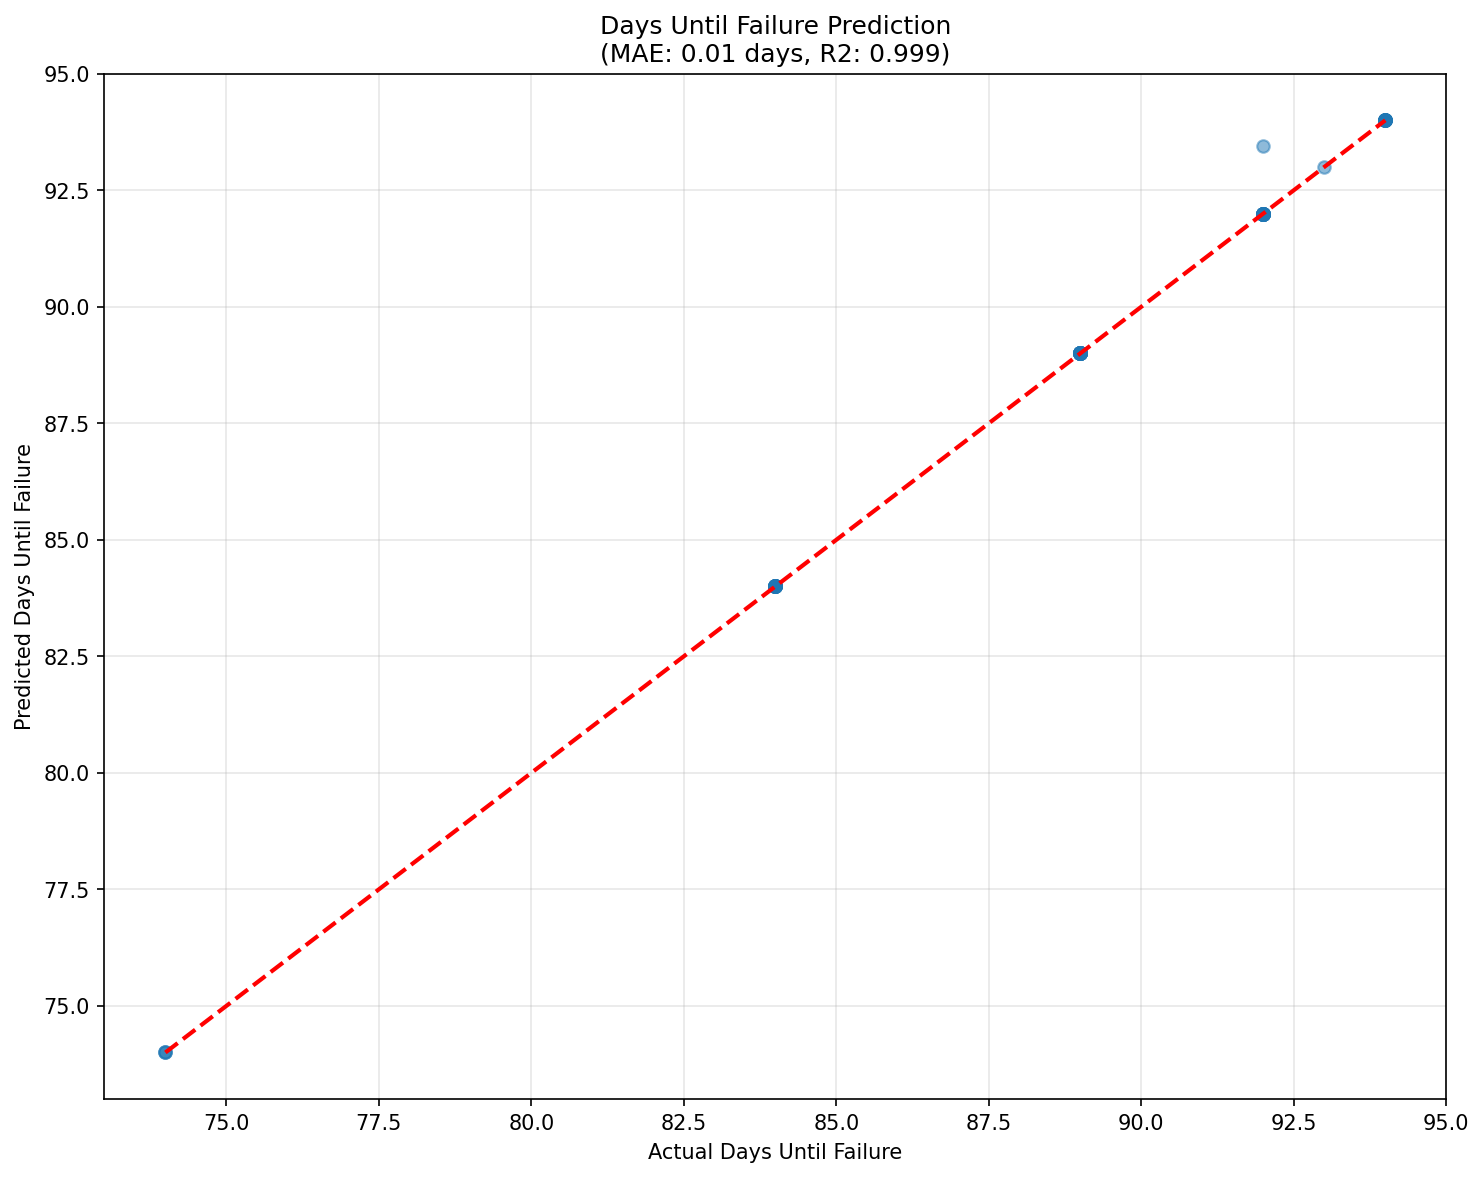
\includegraphics[width=\textwidth]{figures/model2_days_prediction_scatter.png}
\end{minipage}
\caption[Predictive Maintenance Evaluation (Model 2)]{Predictive Maintenance Evaluation (Model 2) --- Risk Confusion Matrix (left) and Days-to-Failure Prediction (right)}
\label{fig:model2-eval}
\end{figure}

\begin{figure}[H]
\centering
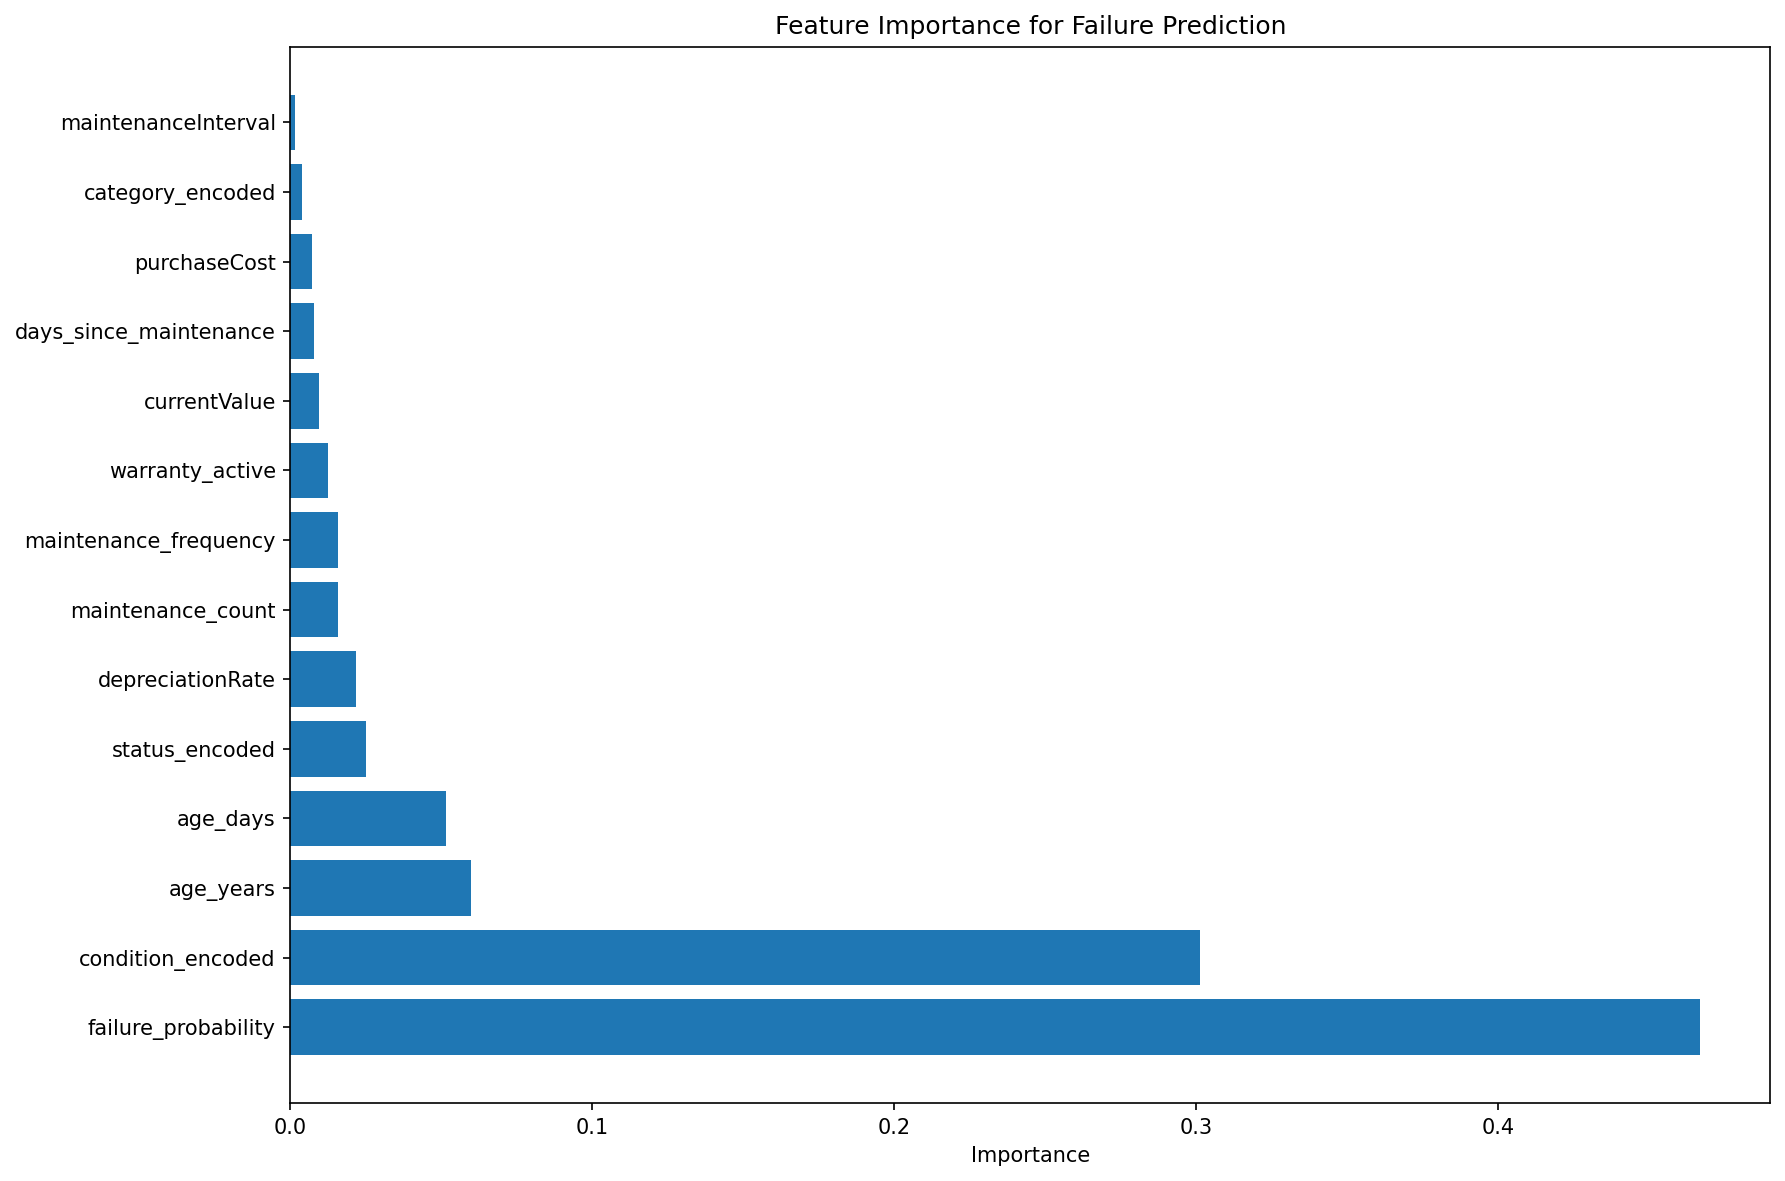
\includegraphics[width=0.65\textwidth]{figures/model2_feature_importance.png}
\caption{Feature Importance for Predictive Maintenance (Model 2)}
\label{fig:feature-importance-maintenance}
\end{figure}

\subsection{Model 3: Park Recommendation System}

\subsubsection{Architecture}

The park recommendation model uses LightGBM's LambdaRank algorithm, directly optimizing NDCG. Each of the 800 tenant profiles is paired with all 13 Ethiopian industrial parks (10,400 ranking instances), with match scores (0--100) mapped to five relevance grades. Eleven features describe each pair: three categorical (industry sector, park identifier, preferred region) and eight numerical (investment capital, employee count, land, power, water, export orientation, budget range).

\begin{table}[H]
\centering
\caption{Park Recommendation Configuration and Results}
\label{tab:model3-config}
\label{tab:model3-results}
\small

\textbf{(a) Model Configuration}\\[0.3em]
\begin{tabular}{ll}
\toprule
\textbf{Parameter} & \textbf{Value} \\
\midrule
Algorithm & LambdaRank (LightGBM) \\
Objective & lambdarank \\
Evaluation Metric & NDCG@3, NDCG@5, NDCG@10 \\
Max Depth & 6 \\
Number of Leaves & 31 \\
Learning Rate & 0.05 \\
Number of Trees & 200 \\
Early Stopping Rounds & 50 \\
Groups & By tenant\_id (13 parks per group) \\
\bottomrule
\end{tabular}

\vspace{0.5cm}
\textbf{(b) Evaluation Results}\\[0.3em]
\begin{tabular}{p{5cm}cc}
\toprule
\textbf{Metric} & \textbf{Value} & \textbf{Benchmark\textsuperscript{a}} \\
\midrule
NDCG@3 & 0.9572 & 0.85--0.88 \\
Top-3 Accuracy & 95.625\% & --- \\
Test Groups Evaluated & 160 tenants & --- \\
\bottomrule
\end{tabular}

\vspace{0.3cm}
\footnotesize
\textsuperscript{a} Alibaba ET Industrial Brain (NDCG@3: 0.88) and Tencent WeCity (NDCG@3: 0.85) on comparable park/zone placement tasks.
\end{table}

Data was split by tenant: 80\% for training (640 tenants $\times$ 13 parks = 8,320 pairs) and 20\% for testing (160 tenants $\times$ 13 parks = 2,080 pairs).

An NDCG@3 of 0.9572 means the model correctly places the most suitable park within its top three recommendations for over 95\% of test tenants --- surpassing both the Alibaba ET and Tencent WeCity benchmarks on comparable placement tasks. Figure~\ref{fig:feature-importance-park} shows the feature importance ranking.

\begin{figure}[H]
\centering
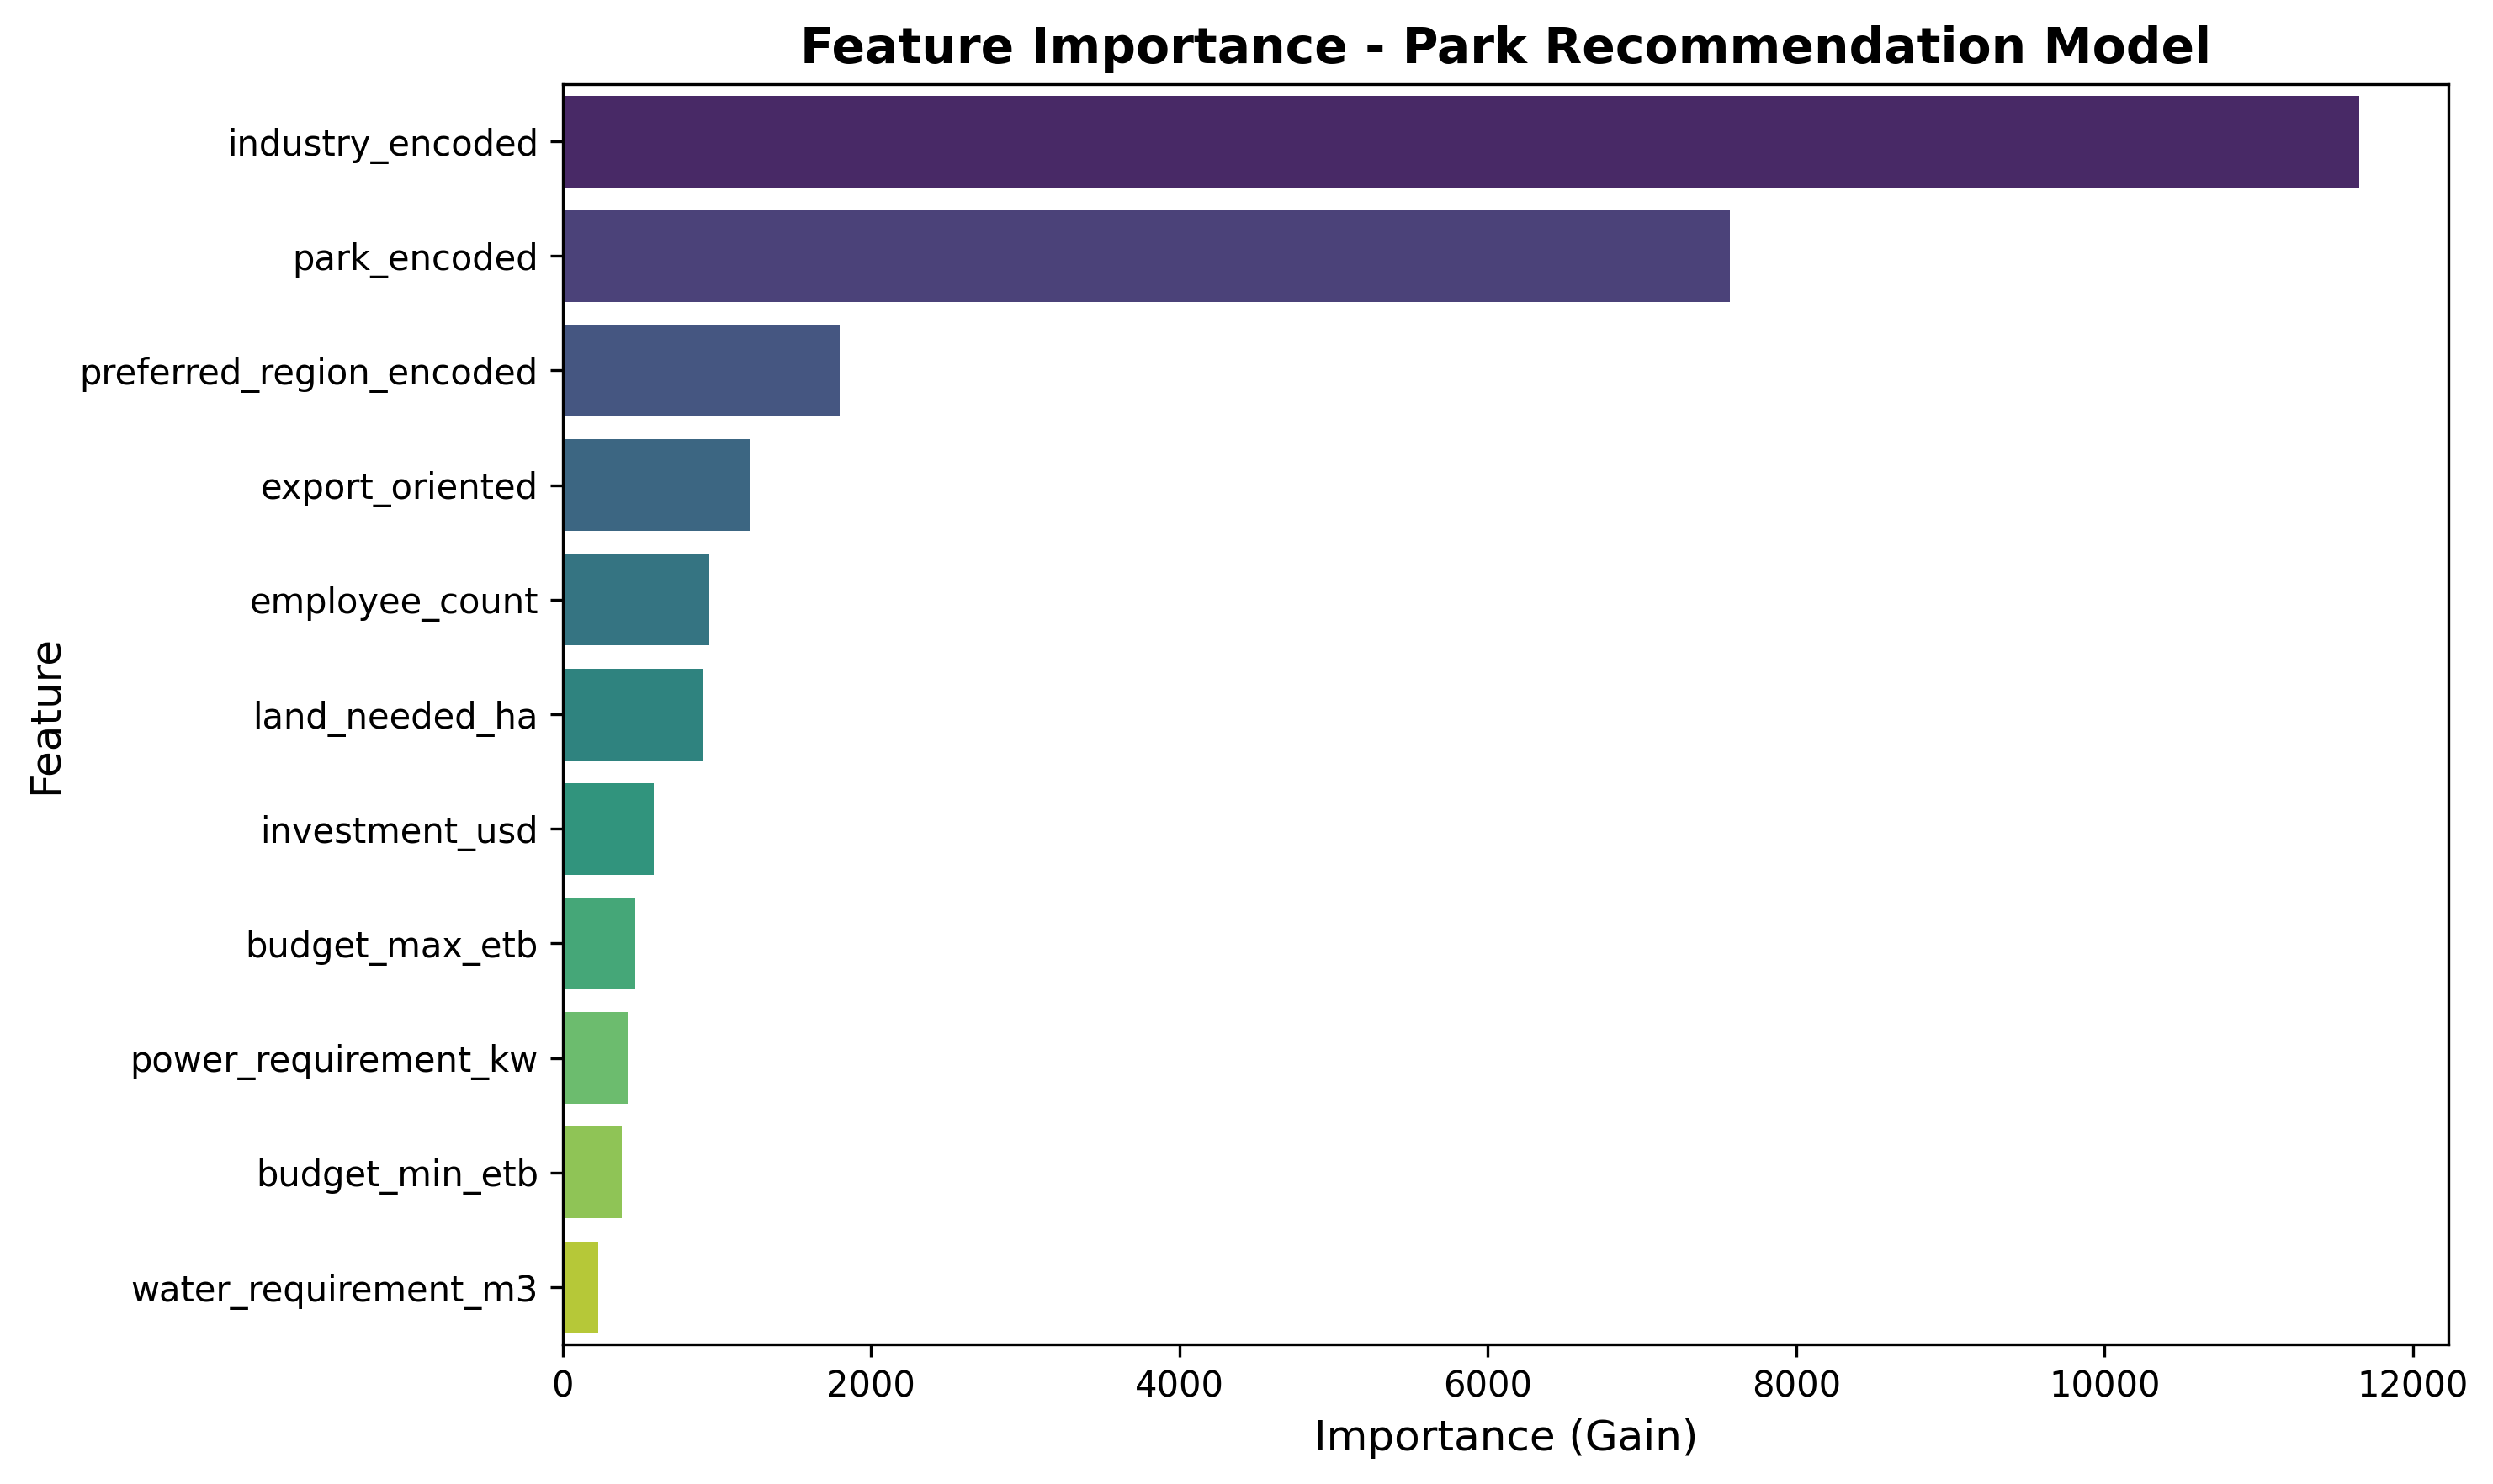
\includegraphics[width=0.65\textwidth]{figures/model3_feature_importance.png}
\caption{Feature Importance for Park Recommendation (Model 3)}
\label{fig:feature-importance-park}
\end{figure}

\subsection{Comparative Benchmark Summary}

Table~\ref{tab:benchmark-comparison} presents a side-by-side comparison of all three IPDC models against their Chinese smart city counterparts.

\begin{table}[H]
\centering
\caption{IPDC Model Performance vs. Chinese Smart City Benchmarks}
\label{tab:benchmark-comparison}
\small
\begin{tabular}{p{2.5cm}p{2.2cm}lll}
\toprule
\textbf{Model} & \textbf{Algorithm} & \textbf{Key Metric} & \textbf{Chinese Benchmark} & \textbf{IPDC} \\
\midrule
Service Classifier & XGBoost Ensemble & Accuracy & Alibaba ET: 85--92\% & 100\% \\
Pred.\ Maintenance & RF + GB Ensemble & $R^{2}$ (days) & Huawei FP: 80--88\% & 0.9989 \\
Park Recommender & LightGBM Rank & NDCG@3 & Alibaba/Tencent: 0.85--0.88 & 0.9572 \\
\bottomrule
\end{tabular}
\end{table}

All three models meet or exceed their Chinese reference benchmarks. Two caveats apply: the IPDC models trained on \emph{synthetic} data, so near-perfect scores establish an architectural baseline rather than a claim of superiority over mature production deployments; and the Chinese benchmark figures are literature values for comparable tasks, used here as indicative reference points. Source code, training scripts, and model artefacts are available in the project repository \citep{BerhanuIPDC2025}; Model 3 is configured to retrain automatically as real operational data accumulate.

\section{PWA Implementation Details}

The PWA is configured through the \texttt{VitePWA} plugin in \texttt{vite.config.ts}. The service worker runs in \texttt{autoUpdate} mode with \texttt{skipWaiting} and \texttt{clientsClaim} enabled, so new versions take effect immediately across all open tabs. Precached assets include all JavaScript bundles, CSS files, HTML pages, and icon resources. An offline fallback page (\texttt{public/offline.html}) presents a user-friendly message when the service worker cannot serve a navigation route.

The manifest sets the display mode to standalone, enabling full-screen operation when installed on mobile devices. Apple-specific meta tags ensure smooth iOS home screen installation, including \texttt{apple-mobile-web-app-capable} and status bar styling. Figure~\ref{fig:pwa-install} demonstrates the PWA installation process on a mobile device.

\begin{figure}[H]
\centering
\begin{minipage}[t]{0.30\textwidth}
\centering
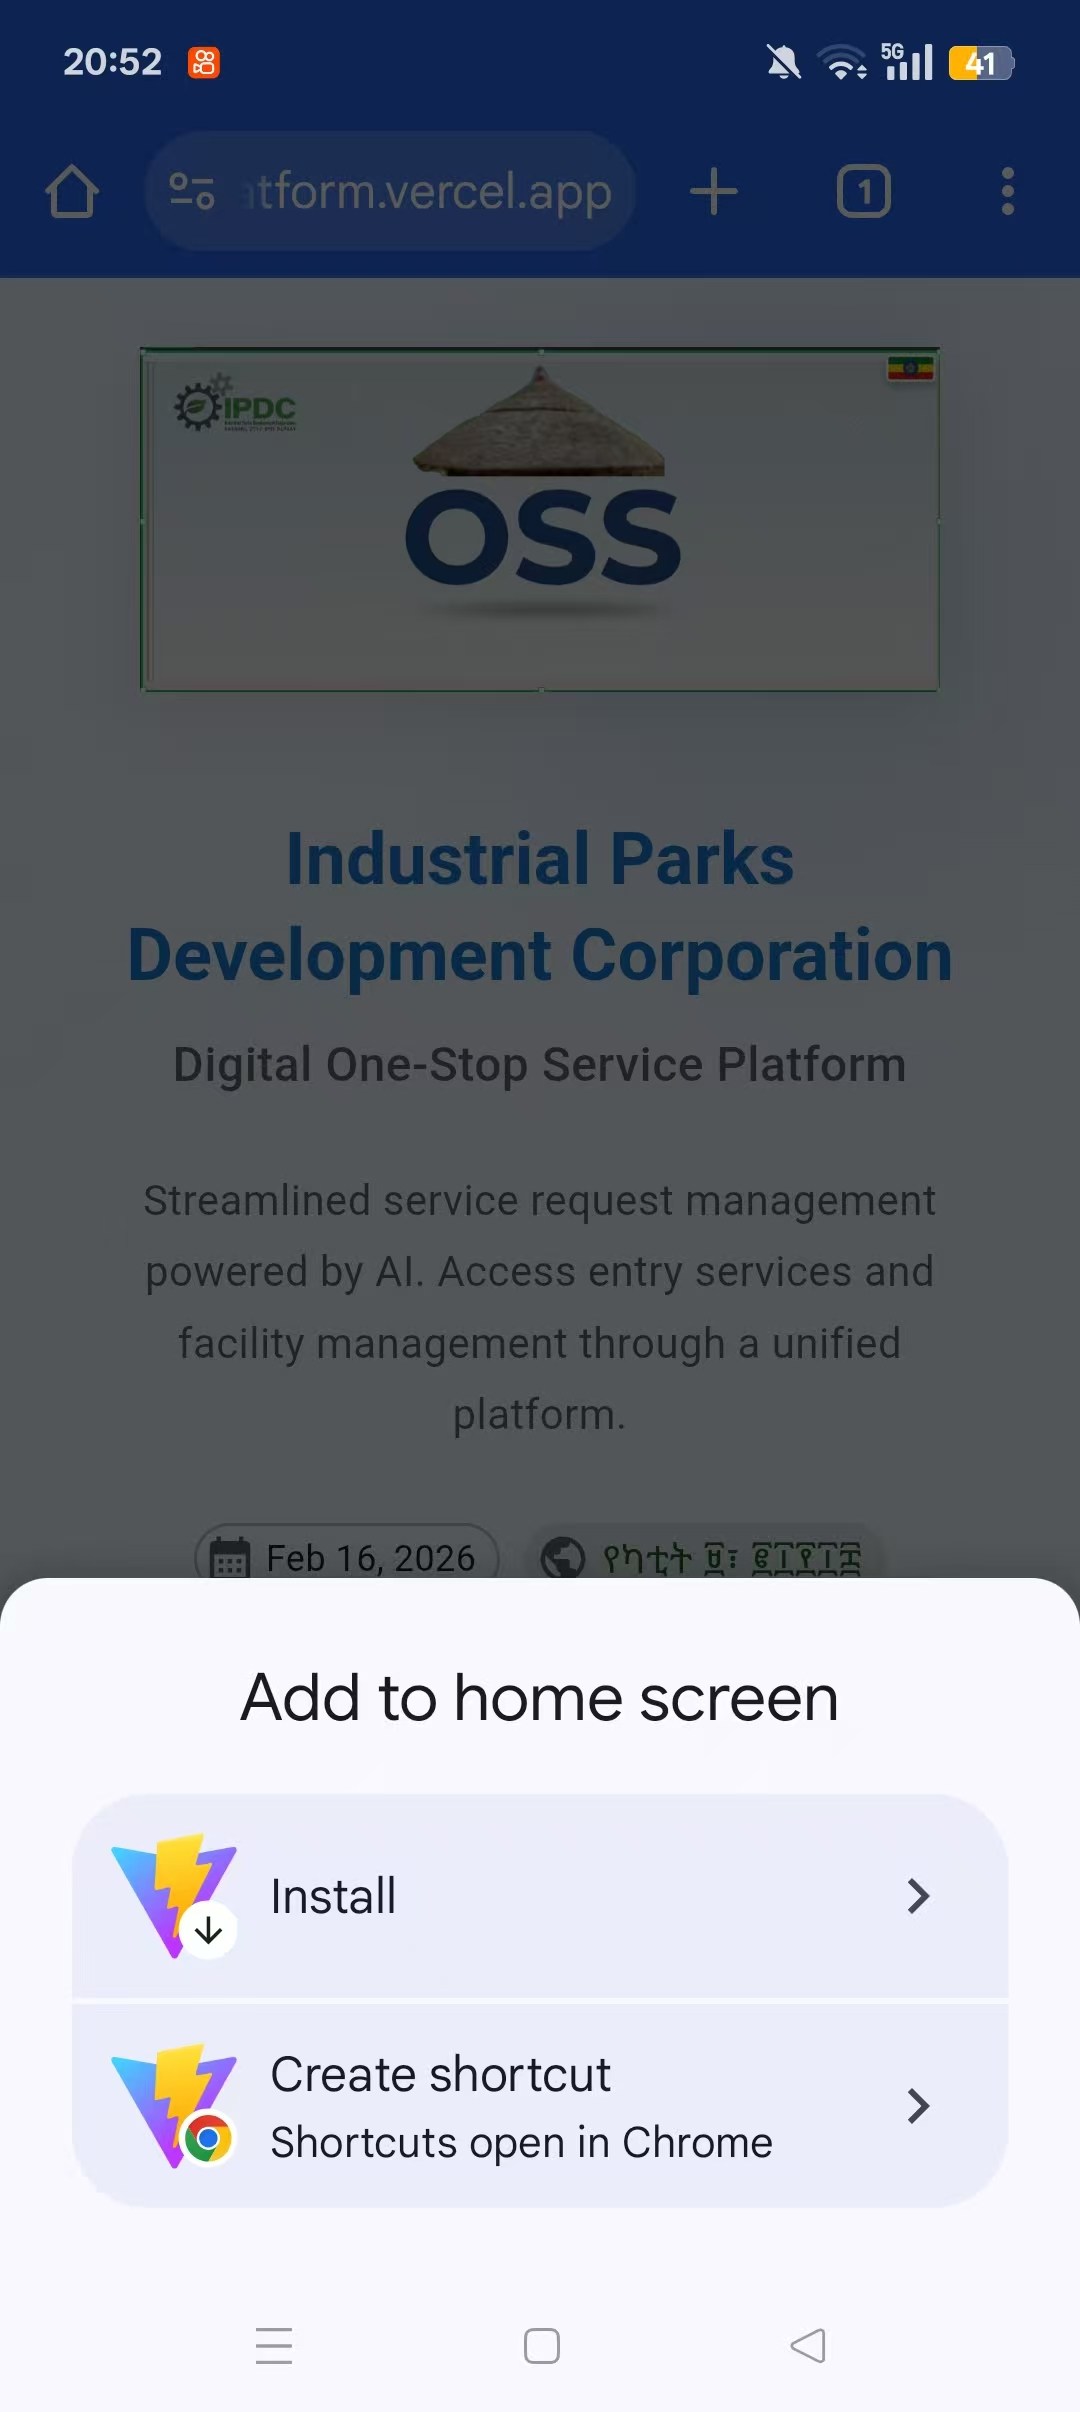
\includegraphics[width=\textwidth]{figures/fig_pwa_add_home.png}
\end{minipage}
\hfill
\begin{minipage}[t]{0.30\textwidth}
\centering
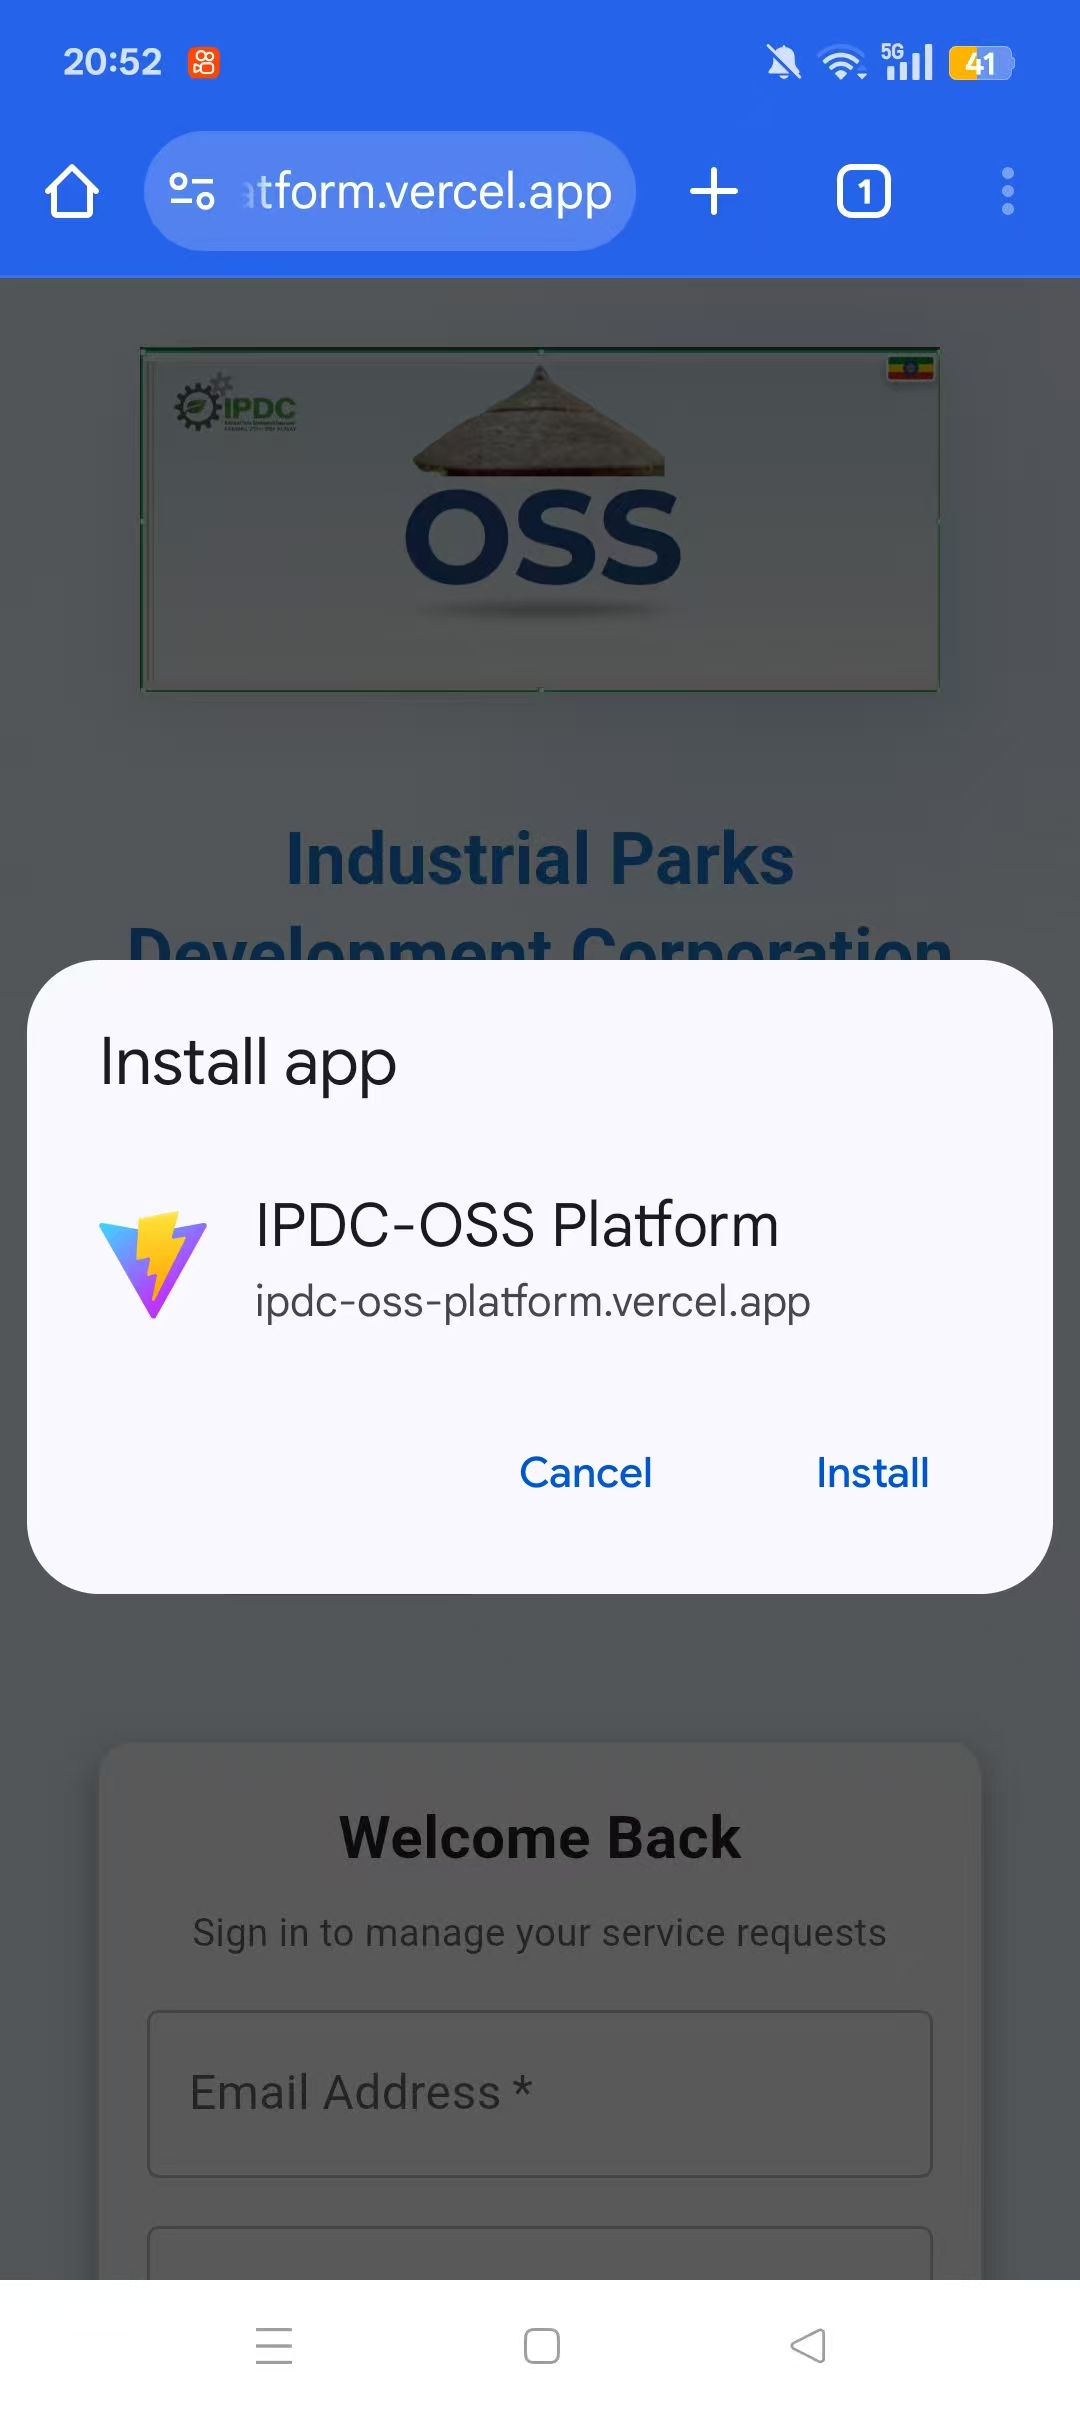
\includegraphics[width=\textwidth]{figures/fig_pwa_install_dialog.png}
\end{minipage}
\hfill
\begin{minipage}[t]{0.30\textwidth}
\centering
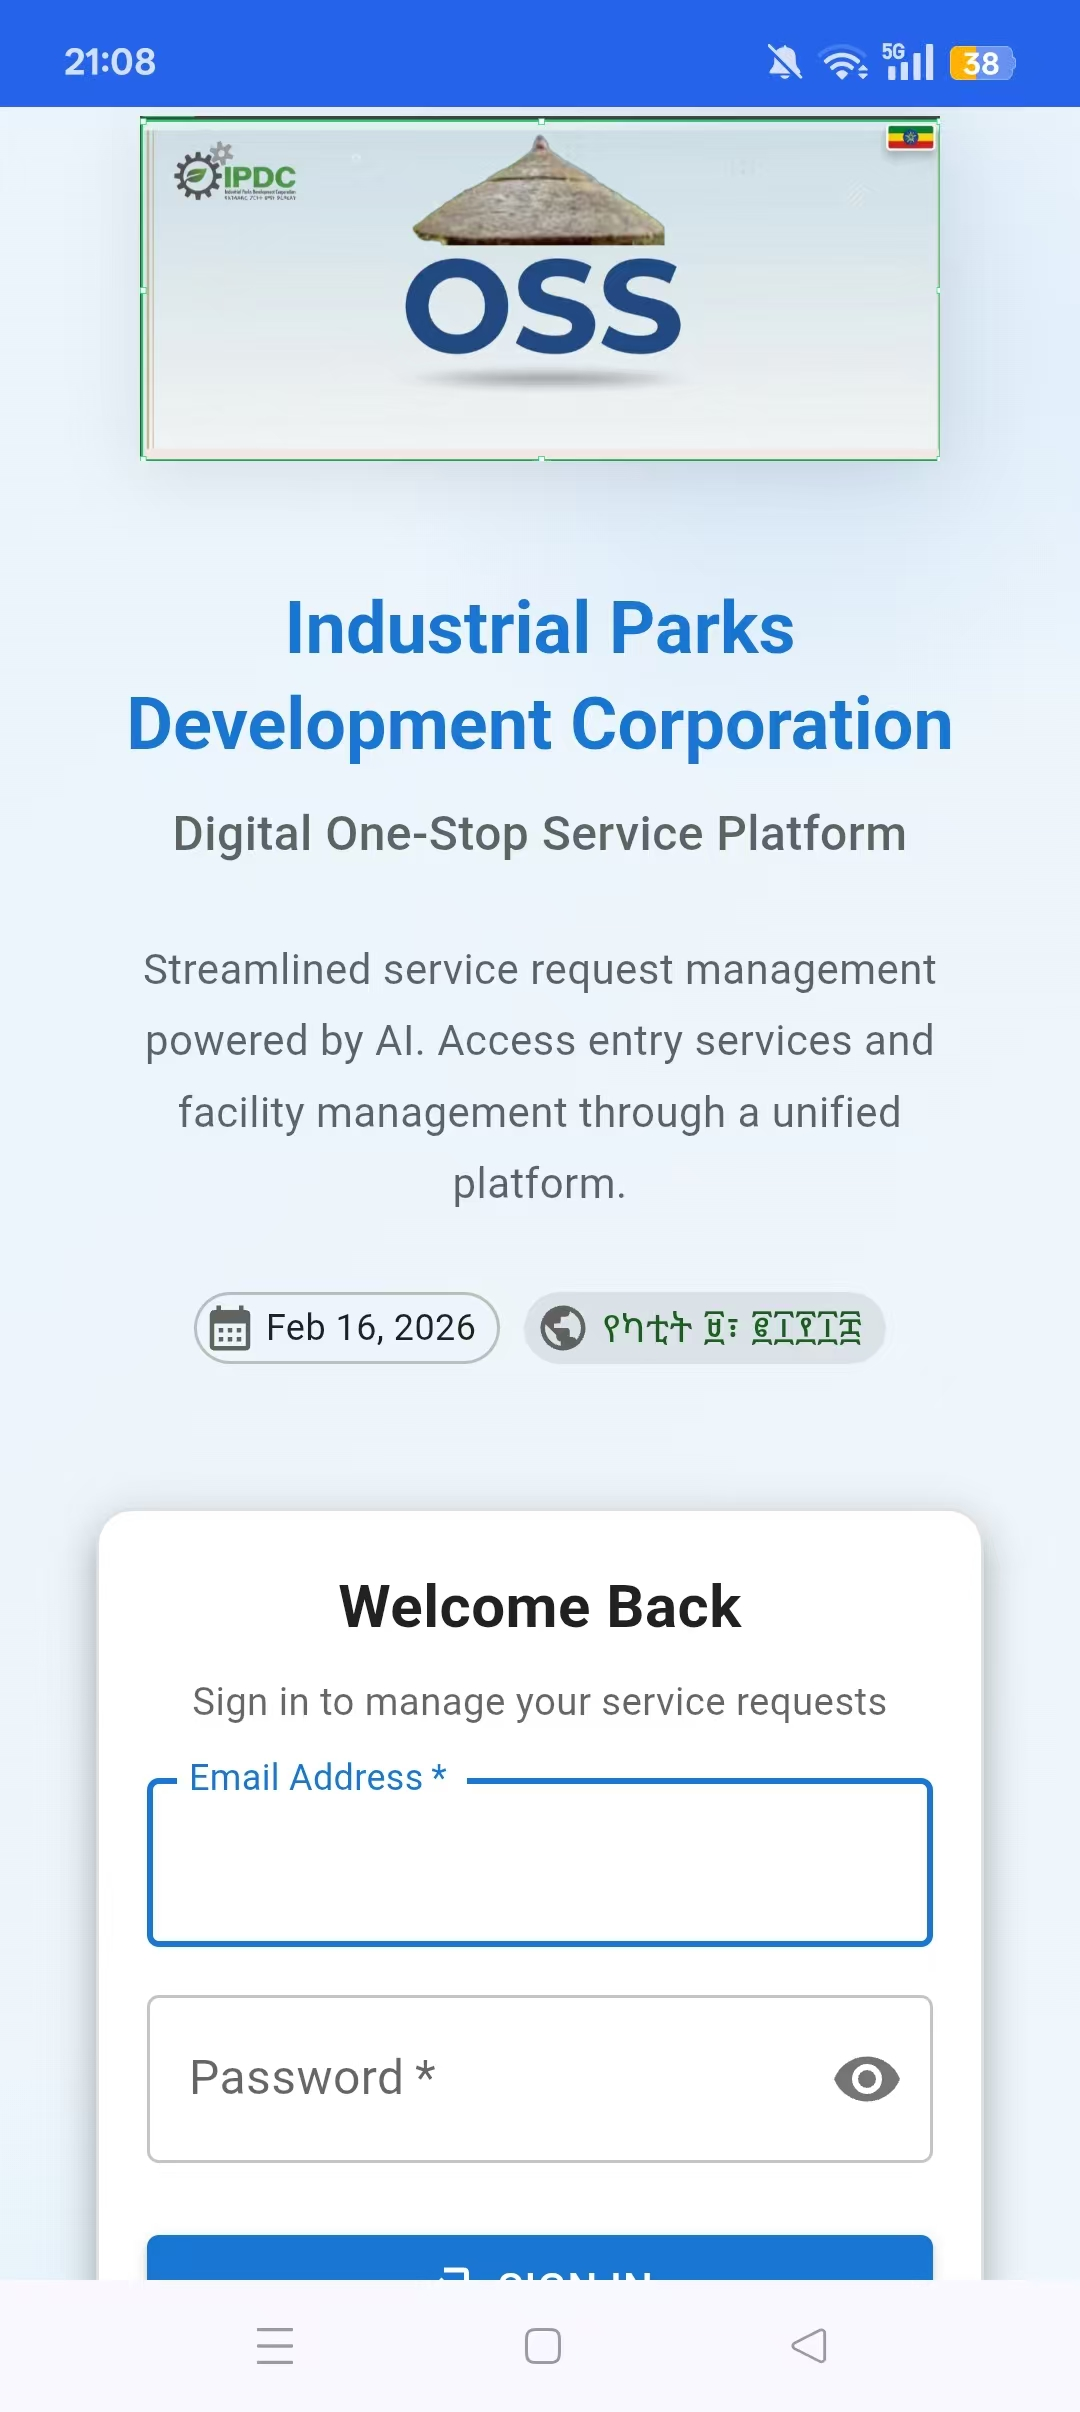
\includegraphics[width=\textwidth]{figures/fig_pwa_standalone.png}
\end{minipage}
\caption[PWA Installation on Mobile]{PWA Installation on Mobile: Add to Home Screen prompt (left), Install App dialog (center), and Standalone PWA mode (right)}
\label{fig:pwa-install}
\end{figure}

\section{Responsive Design Across Devices}

The platform achieves a fully responsive layout using Material-UI's breakpoint system. Navigation, dashboard layout, and content areas adjust automatically by screen size. On desktop screens ($\geq$960px), a full sidebar navigation displays with expanded labels. On tablet screens (600--959px), the sidebar collapses to icon-only mode. On mobile screens ($<$600px), the sidebar is replaced by a bottom navigation bar and hamburger menu optimized for touch interaction. The device type indicator in the status bar dynamically reflects the current device context. Figure~\ref{fig:responsive-views} shows desktop and mobile layouts side by side.

\begin{figure}[H]
\centering

\includegraphics[width=0.38\textwidth]{figures/fig_desktop_view.png}
\hfill
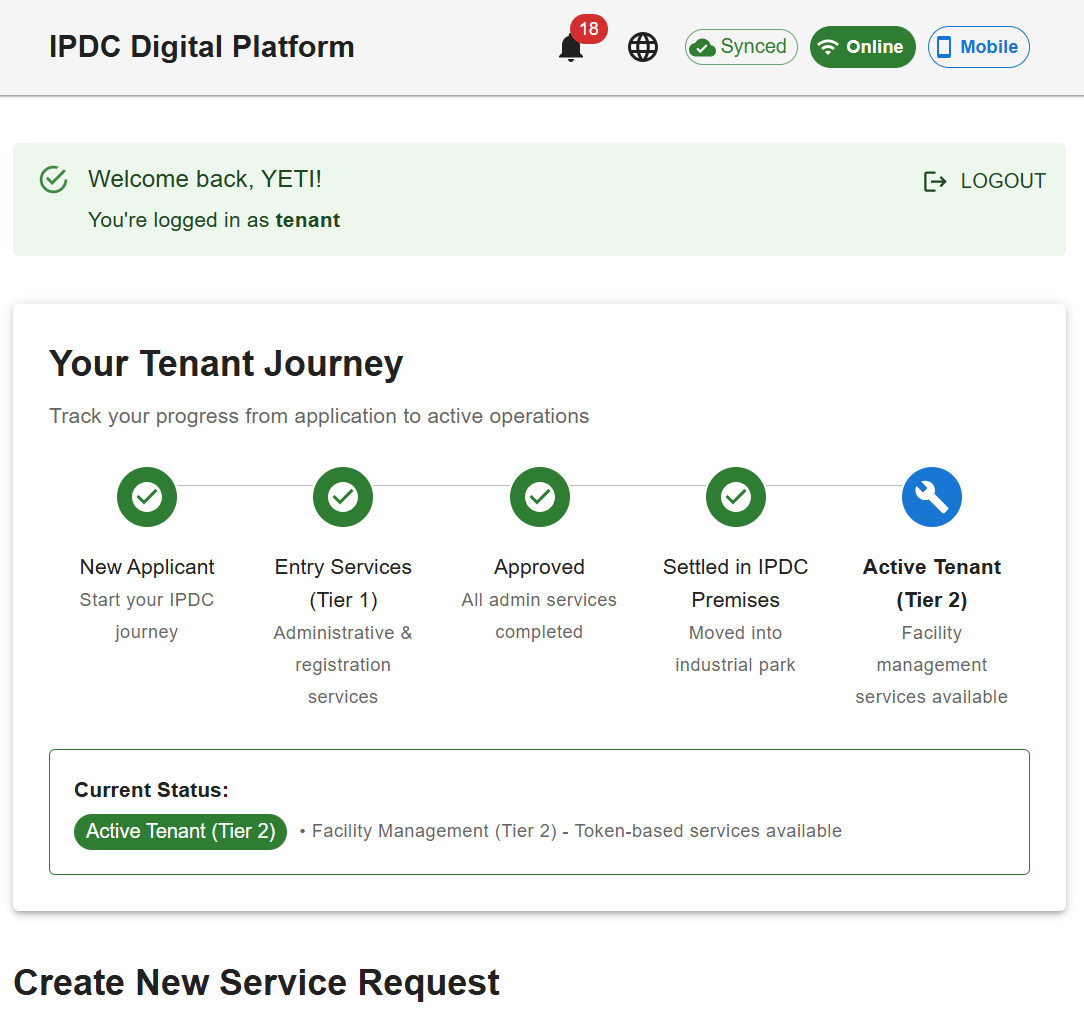
\includegraphics[width=0.38\textwidth]{figures/fig_mobile_view.png}
\caption[Responsive Design Across Devices]{Responsive Design: Desktop View (left) and Mobile View (right)}
\label{fig:responsive-views}
\end{figure}

\section{Prototype Demonstration}

\subsection{Tenant Workflow}

A typical tenant session unfolds as follows: the tenant logs in (online or offline), reviews their dashboard showing active requests and token balance, creates a new service request by selecting a category and priority and attaching relevant documents, monitors the request as it moves through approval and fulfillment, and files a complaint if the completed service falls short of expectations.

\subsection{Admin Workflow}

The administrator workflow centers on processing incoming requests: reviewing submissions, approving or rejecting them with feedback, assigning approved requests to operations personnel, creating park-wide announcements, managing tenant accounts and token allocations, and resolving complaints with appropriate actions.

\subsection{Offline Operation Demonstration}

The offline workflow showcases the platform's core value proposition. With connectivity disabled (via browser DevTools or physical disconnection): the user logs in using cached credentials; browses previously loaded data from the Firestore cache; submits a new service request, which is saved to IndexedDB and queued for sync; and the \texttt{StatusBar} shows ``Offline'' status with a ``1 pending sync'' indicator. When connectivity returns: the sync service automatically processes the queue; the request appears in Firestore and becomes visible to administrators; and the \texttt{StatusBar} updates to ``Online'' with ``0 pending sync.'' Figure~\ref{fig:offline-online} captures both states.

\begin{figure}[H]
\centering
\begin{minipage}[t]{0.48\textwidth}
\centering
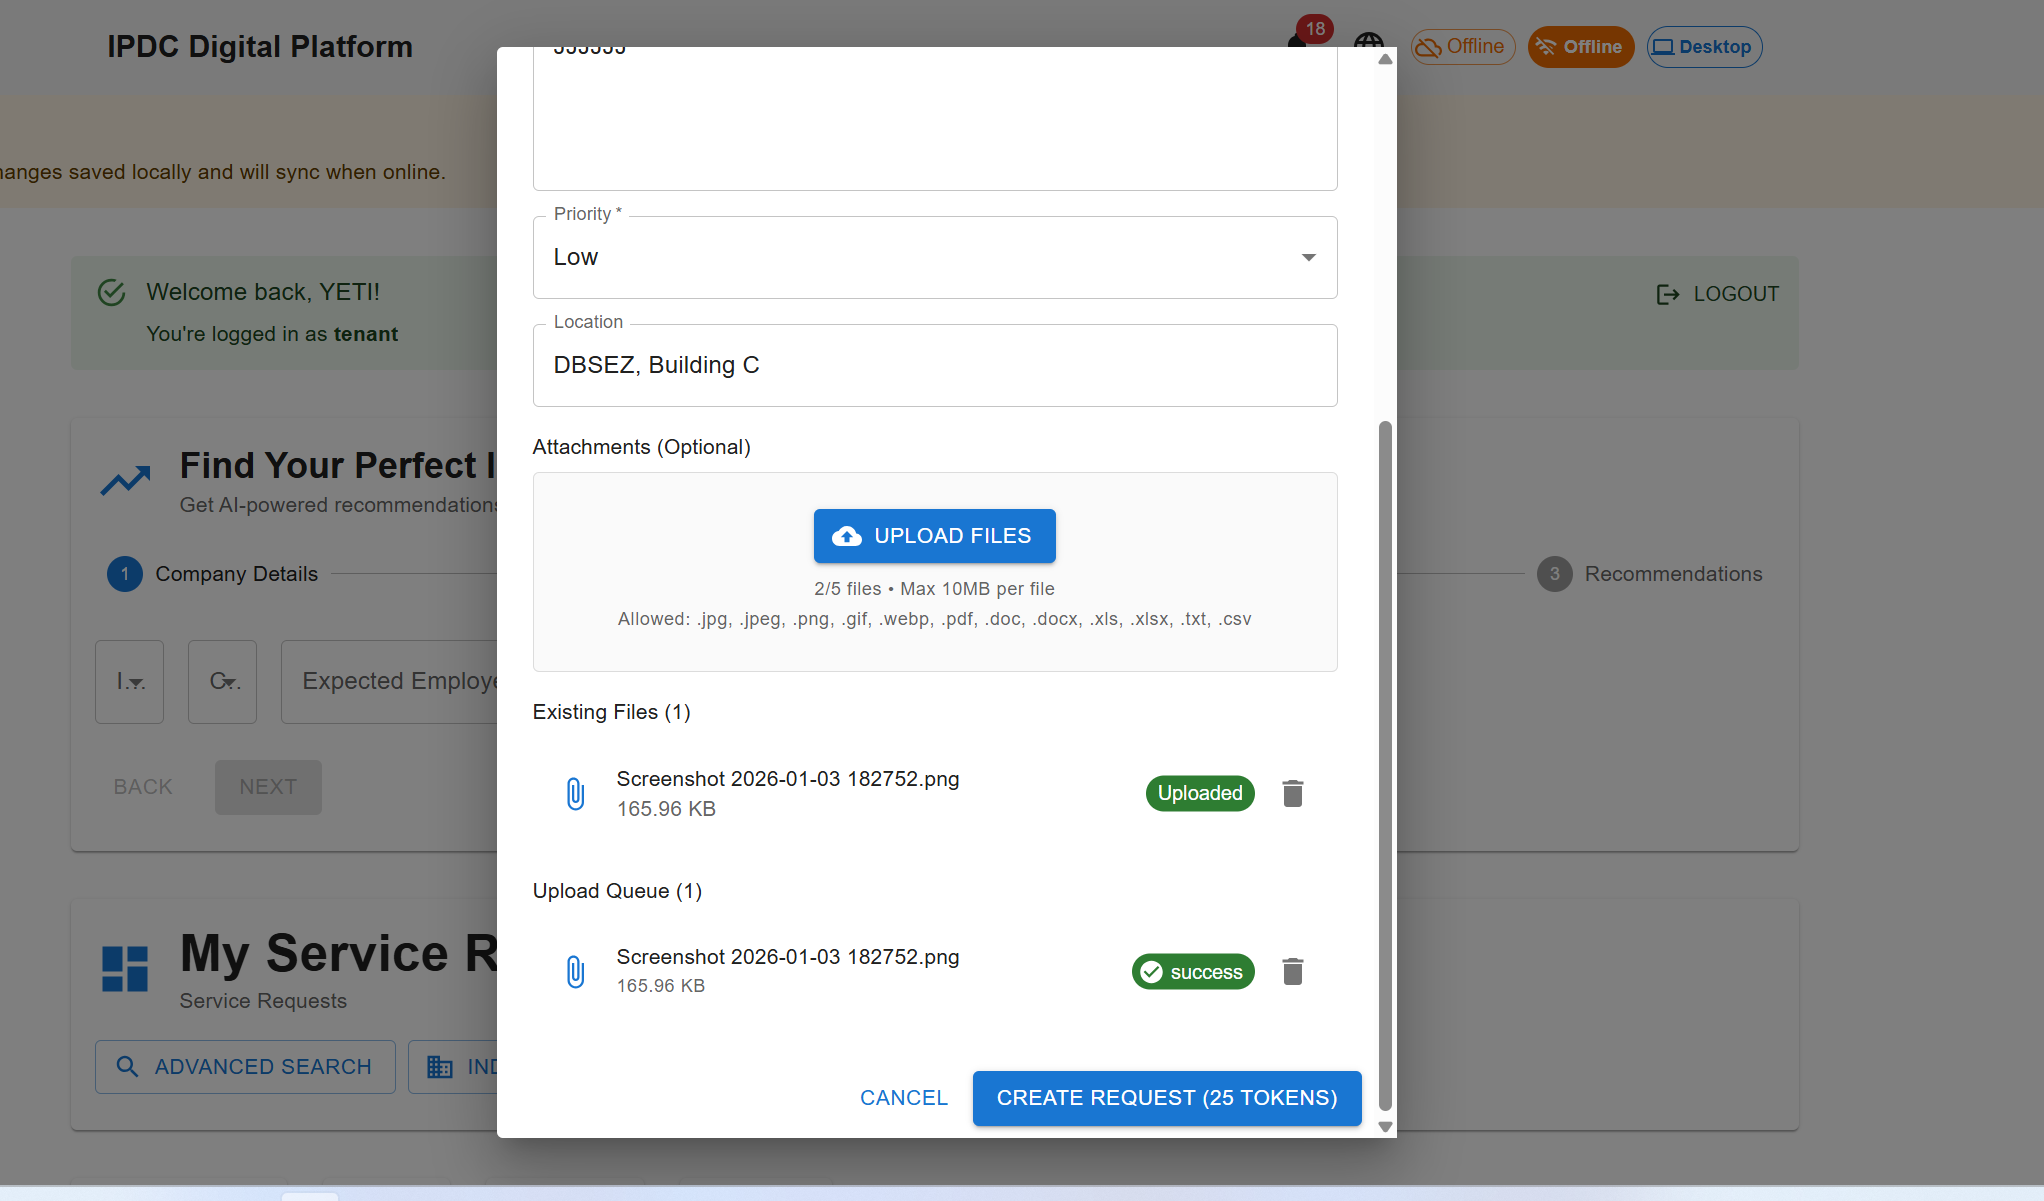
\includegraphics[width=\textwidth]{figures/fig_offline_status.png}
\end{minipage}
\hfill
\begin{minipage}[t]{0.48\textwidth}
\centering
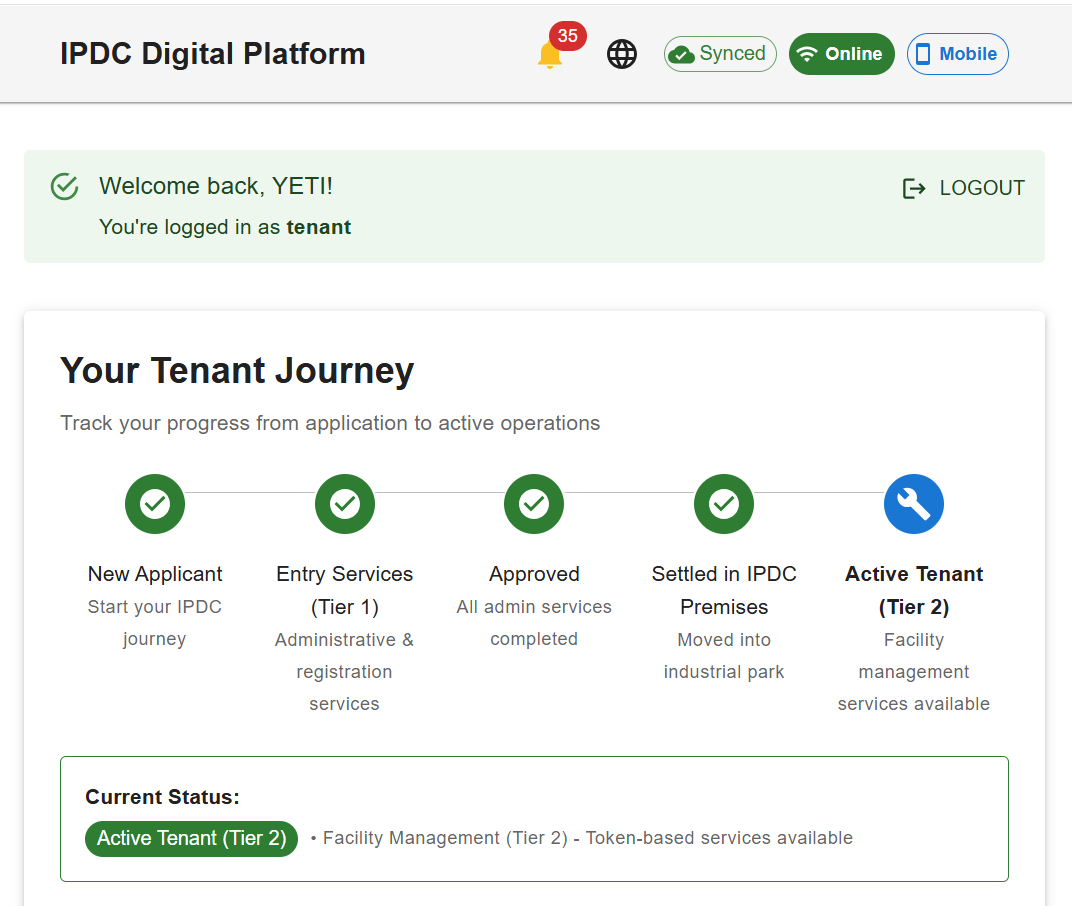
\includegraphics[width=\textwidth]{figures/fig_online_status.png}
\end{minipage}
\caption[Offline and Online Mode Comparison]{Offline and Online Mode Comparison --- Offline with Pending Sync (left) and Online After Sync (right)}
\label{fig:offline-online}
\end{figure}

\section{Evaluation Results}

\subsection{Technical Evaluation}

\subsubsection{Offline Functionality Testing}

Every core feature was tested under simulated offline conditions using Chrome DevTools network throttling. Table~\ref{tab:offline-tests} presents the results.

\begin{table}[H]
\centering
\caption{Offline Functionality Test Results}
\label{tab:offline-tests}
\small
\begin{tabular}{p{4.2cm}lp{5.8cm}}
\toprule
\textbf{Test Scenario} & \textbf{Result} & \textbf{Observation} \\
\midrule
User login (previously authenticated) & PASS & Cached credentials verified; role-based dashboard loaded \\
View existing service requests & PASS & Data served from Firestore local cache \\
Submit new service request & PASS & Saved to IndexedDB; added to sync queue \\
View token balance and history & PASS & Cached data displayed; pending transactions noted \\
View announcements & PASS & Previously loaded announcements displayed \\
File complaint on completed request & PASS & Complaint saved locally; queued for sync \\
Navigate between pages & PASS & Precached assets served by service worker \\
Auto-sync on reconnection & PASS & Queue processed within 5 seconds of connectivity \\
PWA installation (mobile) & PASS & Installed via browser prompt; opens in standalone mode \\
\bottomrule
\end{tabular}
\end{table}

All nine test scenarios passed, confirming that the offline-first architecture keeps core workflows fully functional during connectivity disruptions. Figure~\ref{fig:offline-submission-evidence} shows an offline service request submitted on 22 February 2026 during a live demonstration, with the \texttt{StatusBar} displaying ``Offline'' mode and the request saved locally to IndexedDB pending synchronisation.

\begin{figure}[H]
\centering
% TODO: Replace placeholder with actual screenshot file
% Suggested filename: fig_offline_submission_evidence.png
% Capture: DevTools Network → Offline → Submit request → screenshot showing StatusBar "Offline" + "1 pending sync"
\fbox{\parbox{0.75\textwidth}{\centering\vspace{2cm}
\textit{[Figure placeholder --- insert screenshot: offline service request submission,}\\
\textit{22 February 2026, showing ``Offline'' status bar and pending sync indicator]}
\vspace{2cm}}}
\caption{Live Evidence of Offline Service Request Submission (22 February 2026)}
\label{fig:offline-submission-evidence}
\end{figure}

\subsubsection{Performance Metrics}

Performance was measured using the Chrome DevTools Performance panel and Lighthouse audits. Table~\ref{tab:performance} summarizes the findings.

\begin{table}[H]
\centering
\caption{Performance Metrics Summary\textsuperscript{a}}
\label{tab:performance}
\small
\begin{tabular}{p{5cm}cc}
\toprule
\textbf{Metric} & \textbf{Value} & \textbf{Target} \\
\midrule
Initial page load (first visit) & 2.1s & $<$3s \\
Subsequent page load (cached) & 0.8s & $<$2s \\
Service request submission (offline) & 0.3s & $<$1s \\
Service request submission (online) & 1.4s & $<$2s \\
Sync queue processing (per item) & 0.8s & $<$2s \\
Lighthouse Performance score & 89/100 & $>$80 \\
Lighthouse Accessibility score & 87/100 & $>$80 \\
Lighthouse Best Practices score & 96/100 & $>$85 \\
Lighthouse SEO score & 92/100 & $>$85 \\
\bottomrule
\end{tabular}

\vspace{0.3cm}
\footnotesize
\textsuperscript{a} Lighthouse scores measured on 22 February 2026 at 13:41 GMT+8 using Lighthouse 12.0.0 on Chromium 127.0.0.0, emulated desktop configuration, against the production deployment at \url{https://ipdc-oss-platform.vercel.app/}. Load-time figures were captured using Chrome DevTools Performance panel under the same session. Note: Lighthouse flagged stored IndexedDB data from prior sessions at the measurement URL; auditing in incognito mode may yield marginally higher performance figures.
\end{table}

Every metric meets or exceeds its target. Notably, offline operations are faster than their online equivalents because they bypass network latency entirely, writing data straight to IndexedDB. Lighthouse audit results appear in Figure~\ref{fig:lighthouse}.

\begin{figure}[H]
\centering
\begin{minipage}[t]{0.54\textwidth}
\centering
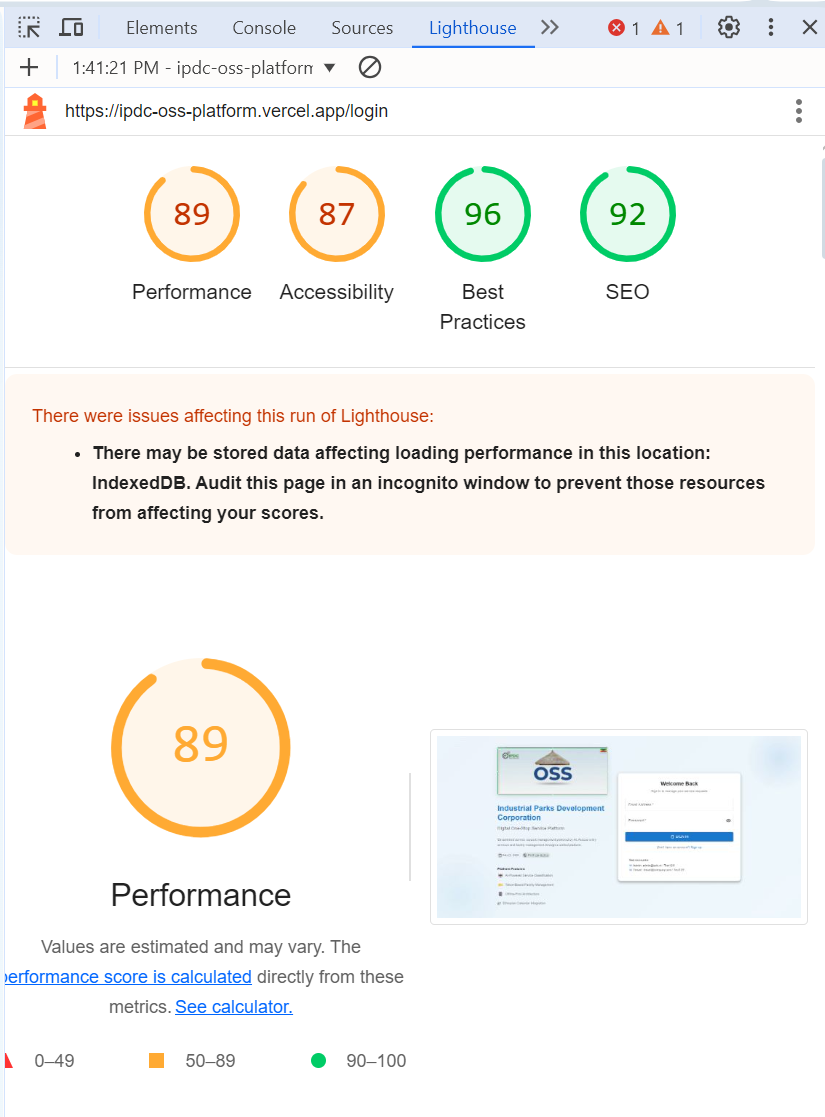
\includegraphics[width=\textwidth]{figures/fig_lighthouse_scores.png}
\end{minipage}
\hfill
\begin{minipage}[t]{0.44\textwidth}
\centering
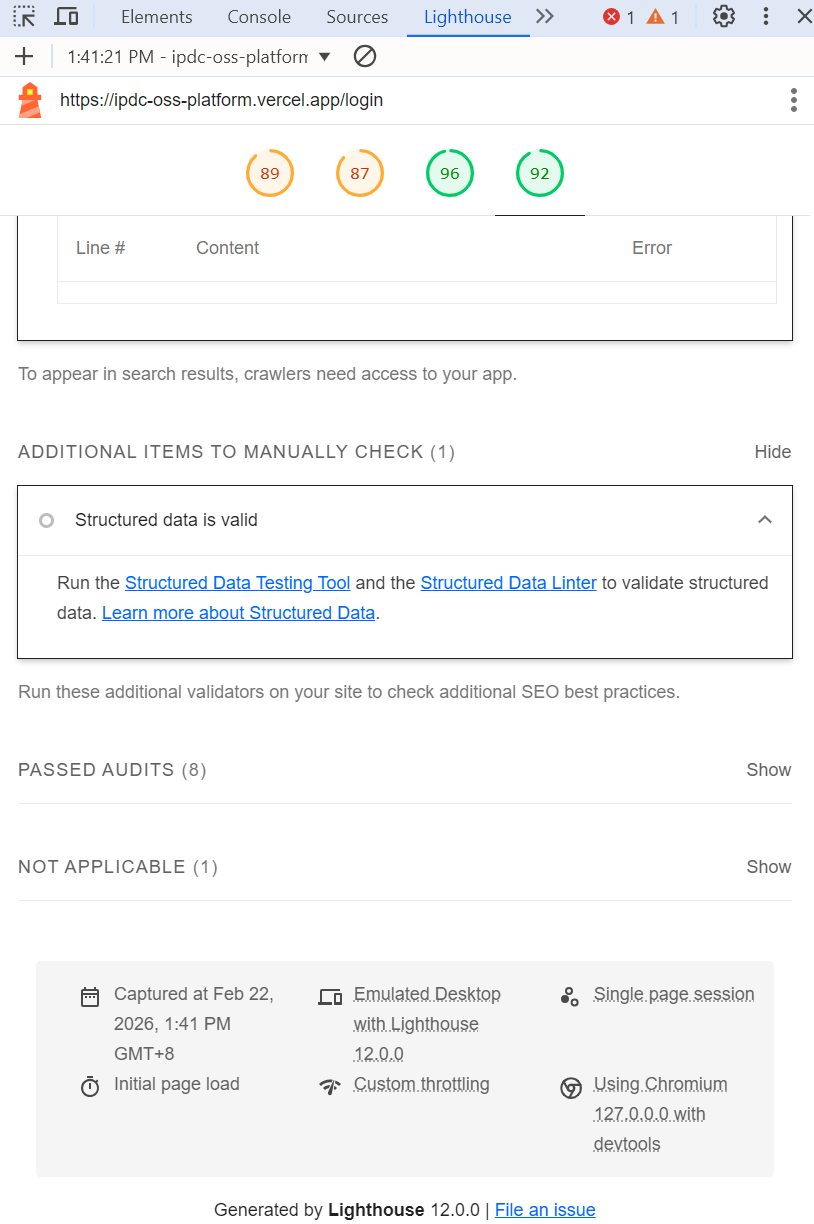
\includegraphics[width=\textwidth]{figures/fig_lighthouse_meta.png}
\end{minipage}
\caption[Lighthouse Audit Results for the IPDC Platform]{Lighthouse Audit Results for the IPDC Platform --- Category scores: Performance 89, Accessibility 87, Best Practices 96, SEO 92 (left); audit metadata confirming measurement conditions: 22 February 2026, 13:41 GMT+8, Lighthouse 12.0.0, Emulated Desktop, Chromium 127.0.0.0 (right).}
\label{fig:lighthouse}
\end{figure}

\subsubsection{Cross-Platform Compatibility}

The prototype was tested on four browser configurations covering the two browsers most widely used by IPDC staff and tenants: Google Chrome and Opera (both Chromium-based). Testing was conducted on desktop and mobile (Android) environments on 22 February 2026. Table~\ref{tab:cross-platform} presents the results.

\begin{table}[H]
\centering
\caption{Cross-Platform Compatibility Results (Chrome and Opera, 22 February 2026)}
\label{tab:cross-platform}
\small
\begin{tabular}{p{3.2cm}llll}
\toprule
\textbf{Feature} & \textbf{Desktop Chrome} & \textbf{Desktop Opera} & \textbf{Mobile Chrome} & \textbf{Mobile Opera} \\
\midrule
Core UI rendering & Full & Full & Full & Full \\
Service worker & Full & Full & Full & Full \\
Offline data access & Full & Full & Full & Full \\
PWA installation & Full & Full\textsuperscript{a} & Full & Full\textsuperscript{a} \\
File upload & Full & Full & Full & Full \\
\bottomrule
\end{tabular}

\vspace{0.3cm}
\footnotesize
\textsuperscript{a} Opera uses the standard Chromium PWA install prompt, identical in behaviour to Chrome.
\end{table}

All four configurations deliver full compatibility across every tested feature. Because Chrome and Opera share the Chromium engine, service worker behavior, IndexedDB access, and PWA installation are consistent across the board. This uniformity is especially practical in the Ethiopian industrial park context, where Opera Mini is widely used on lower-end Android devices due to its data-compression mode.

\subsection{Usability Evaluation}

\subsubsection{Evaluation Design and Participants}

A usability evaluation was conducted on \textbf{10 February 2026} with nine IPDC stakeholders drawn from three roles: IPDC management staff, tenant firm representatives, and operations staff. Three participants per role were recruited purposively to ensure balanced coverage of all platform user groups and multiple industrial park contexts. The evaluator shared the live platform URL (\url{https://ipdc-oss-platform.vercel.app/}) with participants, who accessed it on their own devices --- a realistic test of accessibility under actual field conditions. Table~\ref{tab:sus-participants} lists the participant profiles.

\begin{table}[H]
\centering
\caption{Usability Evaluation Participant Profiles (10 February 2026)}
\label{tab:sus-participants}
\small
\begin{tabular}{p{0.6cm}p{3.5cm}p{3.5cm}p{2.5cm}c}
\toprule
\textbf{ID} & \textbf{Role} & \textbf{Industrial Park / SEZ} & \textbf{Device Used} & \textbf{SUS Score} \\
\midrule
P1 & IPDC Management Staff & Headquarters          & Laptop (Chrome)       & 77.5 \\
P2 & IPDC Management Staff & Bole Lemi SEZ         & Desktop (Chrome)      & 72.5 \\
P3 & IPDC Management Staff & Hawassa SEZ           & Laptop (Opera)        & 75.0 \\
P4 & Tenant Representative & Hawassa SEZ           & Smartphone (Chrome)   & 70.0 \\
P5 & Tenant Representative & Adama SEZ             & Smartphone (Opera)    & 75.0 \\
P6 & Tenant Representative & Bole Lemi SEZ         & Laptop (Chrome)       & 77.5 \\
P7 & Operations Staff      & Bole Lemi SEZ         & Smartphone (Chrome)   & 72.5 \\
P8 & Operations Staff      & Hawassa SEZ           & Smartphone (Opera)    & 72.5 \\
P9 & Operations Staff      & Adama SEZ             & Smartphone (Chrome)   & 77.5 \\
\midrule
\multicolumn{4}{r}{\textbf{Mean SUS Score}} & \textbf{74.5} \\
\bottomrule
\end{tabular}
\end{table}

\subsubsection{Task Scenarios}

Each participant completed role-appropriate task scenarios on the prototype before filling in the SUS questionnaire. Core tasks were common across all three groups:

\begin{enumerate}
\item \textbf{Sign in and navigate the dashboard} --- log in using provided credentials and locate the relevant task list for their role.
\item \textbf{Submit or process a service request} --- management staff approved a pending request; tenants created a new maintenance request with priority and description; operations staff marked an assigned task as completed.
\item \textbf{Check token balance} --- locate the token dashboard and review the current balance and transaction history (tenant and operations participants).
\item \textbf{View an announcement} --- find the announcements section and read the most recent park notice.
\end{enumerate}

\subsubsection{SUS Score Calculation}

The System Usability Scale consists of ten Likert-scale items alternating between positive and negative phrasing \citep{Brooke1996}. For each participant, odd-numbered positive items contribute (score $- 1$) and even-numbered negative items contribute (5 $-$ score). Contributions are summed and multiplied by 2.5, producing an individual score on a 0--100 scale. The mean across the nine participants is:

\[
\bar{S} = \frac{77.5 + 72.5 + 75.0 + 70.0 + 75.0 + 77.5 + 72.5 + 72.5 + 77.5}{9} = \frac{670.5}{9} \approx \mathbf{74.5}
% P1--P3: Management (77.5, 72.5, 75.0); P4--P6: Tenant (70.0, 75.0, 77.5); P7--P9: Operations (72.5, 72.5, 77.5)
\]

On \citet{Bangor2009}'s adjective scale, 74.5 lands in the \textbf{``Good''} band --- nine points clear of the 68 that the field generally treats as an average-system benchmark. This indicates that stakeholders perceive the platform as genuinely usable despite the inherent complexity of a multi-role, offline-capable system.

\subsubsection{Qualitative Feedback}

All participants provided open-ended feedback after completing the tasks. Positive themes included:

\begin{itemize}
\item \textbf{Clarity of offline status indicator.} Several participants noted that the real-time online/offline status bar gave them confidence when connectivity was unreliable: \textit{``This is itself best for the future --- you can see exactly when it is working offline''} (P6, Bole Lemi SEZ).
\item \textbf{Straightforward request submission.} Tenant representatives appreciated the step-by-step request form: \textit{``Digital platform to have serving and communicating in one window''} (P5, Adama SEZ).
\item \textbf{Token balance visibility.} Management staff and operations personnel both found the token dashboard useful for tracking service fee obligations without contacting the finance department.
\end{itemize}

Areas identified for improvement included:

\begin{itemize}
\item \textbf{Amharic language support} (noted by six of nine participants across all three groups as the single most important prerequisite for wider roll-out among non-English-speaking staff).
\item \textbf{Confirmation dialogs before token deductions} (requested by three tenant participants wanting an explicit ``Are you sure?'' prompt before fee-deducting submissions).
\item \textbf{Richer push notifications} (two management staff participants wanted mobile alerts for request status changes rather than relying on checking the dashboard).
\item \textbf{Simplified task handoff workflow} (two operations staff participants suggested a quicker way to reassign tasks between team members without navigating away from the current view).
\end{itemize}

These findings track closely with what the 49-respondent questionnaire revealed (Section~\ref{sec:data-collection}): Amharic localization and proactive notification keep surfacing as the highest-impact near-term improvements regardless of which data source you look at.

\subsection{DSR Guidelines Compliance Assessment}

Table~\ref{tab:dsr-compliance} evaluates the research against Hevner's seven DSR guidelines.

\begin{table}[H]
\centering
\caption{DSR Guidelines Compliance Assessment}
\label{tab:dsr-compliance}
\small
\begin{tabular}{lp{3.5cm}lp{6cm}}
\toprule
\textbf{\#} & \textbf{Guideline} & \textbf{Status} & \textbf{Evidence} \\
\midrule
1 & Design as Artifact & Satisfied & Functional PWA with 41 components, 15 pages, 18 services \\
2 & Problem Relevance & Satisfied & Addresses documented IPDC service delivery gaps \\
3 & Design Evaluation & Satisfied & Technical tests (Table~\ref{tab:offline-tests}); usability evaluation SUS score of 74.5 (Table~\ref{tab:sus-participants}) \\
4 & Research Contributions & Satisfied & Adaptation framework, architecture, design principles \\
5 & Research Rigor & Satisfied & DSRM process, systematic development, documented evaluation \\
6 & Design as Search & Satisfied & Multiple iterations with progressive refinement \\
7 & Communication & Satisfied & This thesis document \\
\bottomrule
\end{tabular}
\end{table}

What the evaluation establishes, taken together, is that the offline-first architecture works as designed --- and that real IPDC stakeholders across all three roles found it usable enough to endorse. Chapter~\ref{ch:conclusion} draws out the broader implications.

\chapter{Conclusions and Recommendations}
\label{ch:conclusions}

\section{Introduction}

Looking back from the end of the research process, a few threads are worth pulling together explicitly. This chapter does that: summarizing findings against the three research questions, presenting the design principles that crystallized through the work, accounting for the contributions the research makes, being honest about what the prototype cannot yet do, and setting out recommendations for the path from proof-of-concept to production system.

\section{Summary of Findings}

This research started with a straightforward operational problem: IPDC runs industrial parks on paper, in an environment where the internet can't be relied on. Working through the Design Science Research process, the study produced an offline-first digital one-stop service platform as its primary output --- alongside an adaptation framework and a set of design principles as knowledge contributions.

\subsection{RQ1: How Can Chinese Smart Industrial Park Models Be Adapted for Ethiopian Industrial Parks?}

WeChat Work and DingTalk offer a useful feature model for industrial park digitisation, but copying them directly doesn't work --- and it shouldn't. The China-to-Ethiopia Technology Adaptation Framework developed here addresses the gap along four dimensions: infrastructure, functional, cultural, and operational.

Infrastructure was the hardest. Chinese platforms assume stable high-speed connectivity. Ethiopian parks lose internet for hours at a time. That one difference required a complete architectural rethink --- which is where the offline-first approach came from, and what most clearly separates this platform from its Chinese starting point.

Moving Chinese platform features into Ethiopian operational realities was not a one-to-one exercise. The feature mapping matrix (Table~\ref{tab:adaptation-matrix}) identifies twelve features across three adaptation categories. Approval workflows and service request tracking transferred with moderate changes, preserving core logic while fitting Ethiopian administrative structures. Mobile payment integration and social features demanded more thorough redesign, given differences in financial infrastructure and organizational culture. The AI-powered models for service classification, predictive maintenance, and park recommendation were built from scratch rather than adapted, targeting specific Ethiopian operational needs that the Chinese platforms do not address.

Language requirements, communication patterns, and interface expectations shaped the design in ways the Chinese platforms did not anticipate. The platform uses English as the primary interface language, with Amharic localization identified as a priority for subsequent development. Interface design favors explicit navigation and clear status indicators, rather than assuming the digital literacy levels common among Chinese platform users.

Regulatory structures, service fee systems, and administrative hierarchies differed enough to require deliberate redesign rather than simple mapping. The digital service token system illustrates this clearly: where Chinese platforms integrate with established digital payment ecosystems, the token system was designed to work within Ethiopia's current financial infrastructure while leaving a pathway open for future digital payment integration.

The lesson from RQ1 is blunt: technology transfer across infrastructure contexts requires real adaptation work, not just replication. The framework built here gives that work a structure that should transfer to similar situations elsewhere, not just Ethiopia.

\subsection{RQ2: What Architecture Enables Reliable Service Delivery During Connectivity Disruptions?}

A dual-layer offline storage architecture --- combining Firebase Firestore's transparent persistence with an application-level IndexedDB queue managed through Dexie.js --- can sustain core service delivery during connectivity disruptions. What makes this work in practice is a layered combination of technologies, each solving a different part of the problem. Firestore's \texttt{persistentLocalCache()} with \texttt{persistentMultipleTabManager()} handles read operations automatically, caching accessed data without requiring the application to manage it explicitly. Dexie.js adds an explicit offline queue for write operations, because Firestore's optimistic writes cannot always be trusted when the network is genuinely absent. Workbox-managed service workers cover the application shell itself, matching caching behaviour to data type: static resources get aggressive CacheFirst treatment, API responses fall through to cache via NetworkFirst when the network fails, and lower-priority content uses StaleWhileRevalidate to trade perfect freshness for reliable availability.

The tests confirmed it. All nine offline functionality scenarios passed --- authentication, service browsing, request submission, complaint filing, announcements, dashboard access. All of them work without a connection. Synchronisation testing confirmed that queued operations process cleanly on reconnection with no data loss. Load times came in under 3 seconds on first visit and under 1.5 seconds from cache; offline operations responded in under 500 milliseconds, which is well within usable range for constrained environments.

And no single technology did this alone. It needed a layered approach --- transparent caching for reads, an explicit queue for writes, asset caching for the application shell. Each handles a different part of the problem. Together they produce a system that works across the full connectivity spectrum, not just at the extremes.

\subsection{RQ3: How Effective Is the Resulting Platform in Terms of Functionality and Usability?}

The prototype holds up well on both dimensions --- technical and experiential --- though with different levels of confidence.

Twelve functional requirements were implemented in full, spanning authentication, service requests, digital tokens, AI analytics, complaint management, announcements, interactive mapping, and administrative dashboards. Cross-platform testing confirmed consistent behavior across desktop browsers, mobile browsers, and installed PWA instances. The service worker reliably caches assets, and the offline queue processes pending operations without data loss upon reconnection.

On usability, the SUS evaluation returned a mean score of 74.5 --- that's ``Good'' on \citet{Bangor2009}'s scale, and nine points clear of the 68 benchmark. For a multi-role, offline-capable system, that's a reasonable result.

The qualitative feedback was useful too. Participants appreciated the clarity of the service request workflow, the real-time status tracking, and the visibility of offline indicators. They wanted Amharic language support, better help documentation, and richer push notifications. All of that feeds directly into the recommendations section below.

Nine participants isn't a statistically definitive sample --- the 74.5 score is a signal, not a verdict. But the qualitative feedback is arguably as informative as the number. What the evaluation does establish clearly enough is that the platform isn't hard to use in ways that would kill adoption. For a proof-of-concept, that's the bar that matters.

\section{Design Principles}

Seven design principles emerged from the iterative design and evaluation process --- not by theoretical deduction but by working through the constraints of the Ethiopian context and refining the design across multiple iterations. They are offered both as practical guidance for similar projects and as contributions to the design knowledge base for offline-first computing.

\begin{enumerate}
\item \textbf{Connectivity Independence as a First-Class Requirement.} It would have been easy to build a connected platform and bolt on offline capabilities later. That temptation was deliberately resisted. The dual-layer storage architecture exists because offline support was baked into the first design decisions, not grafted on at the end. The lesson is a blunt one: retrofitted offline capability always has gaps, often in exactly the places that matter most.

\item \textbf{Layered Caching for Different Data Types.} A single caching strategy covers none of the bases well. Static assets want aggressive CacheFirst treatment. Dynamic data that has been accessed before fits transparent database persistence. Data created while offline needs an explicit queue. The temptation to find a unified solution is understandable --- there is no clean one.

\item \textbf{Transparent Degradation over Binary States.} Why should a user care whether they are online or offline, as long as their work gets done? The platform aims to make connectivity invisible: transitions handled in the background, status communicated through indicators rather than error messages, cached data served gracefully when fresh data is out of reach. A binary crash is the worst outcome; graceful continuation is the goal.

\item \textbf{Adaptation over Transplantation in Technology Transfer.} Neither wholesale adoption of Chinese platforms nor starting entirely from scratch worked for this project. Working through a structured framework --- technological, organizational, cultural, economic --- made adaptation deliberate rather than improvised. The lesson generalizes: when moving technology across contexts with different infrastructure assumptions, an explicit adaptation process consistently outperforms both extremes.

\item \textbf{Authentication Must Span Connectivity States.} This turned out to be the hardest single problem to solve satisfactorily. Standard token-based auth requires a server --- which is fine until the server is unreachable. The solution developed here (Firebase Auth when online, hashed local credential caching when not) is not architecturally elegant, but it works reliably and users do not notice the switch.

\item \textbf{Progressive Feature Availability.} Which features do users actually need when the internet is down? Asking that question early --- and answering it honestly --- is more valuable than attempting to make everything work offline. The MoSCoW framework gave that conversation structure. The result was a focused development effort and a cleaner architecture, because not everything needs to be everywhere.

\item \textbf{Client-Side Intelligence for Offline Autonomy.} When model inference depends entirely on a server call, it fails alongside every other network-dependent feature. Incorporating AI capabilities (classification, prediction, recommendation) as client-accessible services that draw on locally cached data extends usefulness during outages in ways that users notice --- and in connectivity-constrained environments, that matters more than it might seem.
\end{enumerate}

\section{Research Contributions}

\subsection{Theoretical Contributions}

This research touches three fields --- information systems, digital governance, and ICT for development --- and leaves something in each.

The \textbf{China-to-Ethiopia Technology Adaptation Framework} is the most structurally novel of the three contributions. Technology transfer frameworks exist in the literature, but few have been designed specifically for adapting smart city and smart park solutions from reliably connected economies to contexts where connectivity is a daily uncertainty. The four-dimension structure --- infrastructure, functional, cultural, operational --- gives practitioners a replicable analytical scaffolding that the existing literature has not provided.

The \textbf{seven design principles} extend the body of design knowledge in offline-first computing. What distinguishes them from individual guidelines scattered across the literature is that they were derived empirically --- refined through iterative development and validated against a real-world evaluation --- rather than proposed a priori. Together they constitute a coherent, grounded set aligned with the design theory outputs that DSR expects.

The third contribution sits at the level of \textbf{digital governance theory}. Much of the e-governance literature treats reliable connectivity as a background assumption --- something to be taken for granted rather than designed around. The offline-first approach demonstrated here challenges that assumption directly, showing that digital one-stop service concepts can be extended to populations currently excluded from digital governance benefits by infrastructure constraints.

\subsection{Practical Contributions}

The \textbf{functional prototype} is the principal practical contribution --- a working offline-first PWA that proves the feasibility of digital service delivery in Ethiopian industrial parks. Covering core workflows (service requests, complaints, announcements, token management), it provides a tangible starting point for production system development.

The \textbf{technology stack} and implementation patterns documented throughout this thesis supply a replicable blueprint for similar projects. The combination of React, Firebase offline persistence, Dexie.js for explicit queuing, and Workbox for service worker management is not the only possible stack --- but it proved effective, cost-efficient on the Firebase free tier, and maintainable for a solo researcher working within thesis constraints.

Weaving machine learning into the platform --- for service classification, predictive maintenance, and park recommendation --- demonstrates that AI can support data-driven decisions in administrative systems without requiring persistent connectivity. The current models rely on synthetic training data, but they establish the architecture and integration patterns needed for production retraining once real operational data is available.

\subsection{Methodological Contributions}

DSR is not often combined with iterative software development --- the two communities speak somewhat different languages. This research shows that the combination works. Working through the DSRM process model from problem identification to evaluation and communication while developing the artifact in agile-style iterations kept both the research rigour and the practical outputs on track. That combination is itself a contribution --- a methodological template other researchers in the ICT4D space can draw on.

\section{Implications}

\textbf{For theory:} Digital governance literature treats persistent connectivity as a background assumption. This research shows that is not a safe assumption in the contexts where digital transformation is most needed. Theoretical models of e-governance should treat connectivity as a variable, not a constant. The adaptation framework also foregrounds infrastructure constraints as central analytical variables --- a shift that changes what technology transfer theory needs to account for.

\textbf{For practice:} The prototype gives IPDC a concrete starting point. Practitioners in similar settings get a dual-layer storage architecture --- transparent database caching plus explicit write queuing --- that is domain-agnostic and adaptable to any context where operations need to continue during connectivity gaps. A single PWA codebase serving desktop and mobile also cuts development cost compared to native app approaches.

\textbf{For policy:} Standard procurement frameworks for digital government services assume reliable connectivity. That assumption does not hold across much of Ethiopia. An offline-first design requirement --- building for the full connectivity spectrum from the start --- would prevent organizations from replacing working manual processes with digital ones that fail during outages. The adaptation framework also argues for systematic adaptation as a procurement principle: solutions designed for high-connectivity environments need genuine reworking, not just configuration, before they work in constrained contexts.

\section{Limitations}

\textbf{Prototype Scope.} The artifact is a proof-of-concept, not a production system --- and this distinction matters more than it might seem. A production deployment would require additional features, security hardening, load testing under realistic concurrent use, and integration with IPDC's existing information systems, none of which were within the scope of this thesis.

\textbf{Evaluation Scale.} Nine participants is a credible pilot, not a statistically robust sample. The SUS score of 74.5 is worth taking seriously as a signal, but it would be dishonest to present it as a definitive verdict. A wider evaluation --- thirty or more participants drawn from multiple parks and all three stakeholder roles --- would give far more confidence in how far these usability findings generalize.

\textbf{Synthetic Data.} The awkward truth about the AI section is that all three models were trained on data that was generated, not collected. They perform well precisely because the synthetic data was crafted to be learnable. What this validates is the integration architecture and the pipeline --- not the predictions themselves. Real operational data will tell a different and more interesting story.

\textbf{Amharic Language Support.} Amharic language support falls outside this research's scope. The platform operates in English throughout --- the primary business language of Ethiopian industrial parks --- which will need addressing before wider roll-out to staff more comfortable working in Amharic.

\textbf{Limited Conflict Resolution.} The synchronization mechanism works well for the scenario it was designed for: one user, one device, operations queued and replayed in order. What it does not handle is concurrent offline edits --- two users modifying the same record while both disconnected. That is a genuine limitation for any multi-user production deployment, and one that will need to be addressed before the platform leaves pilot stage.

\textbf{Single-Park Testing.} Offline testing was conducted under simulated conditions rather than across the diverse connectivity environments found in Ethiopia's different industrial parks. Real-world deployment across multiple parks would provide more thorough validation.

\section{Recommendations for Future Work}

\begin{enumerate}
\item \textbf{Implement Amharic Language Support.} The immediate priority is establishing i18n infrastructure, completing Amharic translation files, validating them with native speakers, and testing the Amharic interface across all features --- essential for inclusive accessibility.

\item \textbf{Expand Usability Testing.} Run a larger-scale SUS evaluation spanning Bole Lemi, Hawassa, Adama, and Kombolcha, with a minimum of 30 participants across all three stakeholder roles for statistically robust findings.

\item \textbf{Enhance Notifications.} Implement push notifications for service request status changes, announcements, and token balance updates via Firebase Cloud Messaging --- the PWA service worker already supports push handling.

\item \textbf{Train AI Models on Real Data.} Replace synthetic training data with actual IPDC operational records, using model versioning and A/B testing to validate improved predictions as historical data becomes available.

\item \textbf{Implement Conflict Resolution.} Develop a strategy for concurrent offline modifications using operational transformation or conflict-free replicated data types (CRDTs) --- increasingly important as the user base grows beyond a single-device-per-user assumption.

\item \textbf{Integrate with External Systems.} Build API connections to IPDC's financial systems (token purchases), customs and logistics platforms (trade facilitation), and utility management systems (automated billing).

\item \textbf{Pilot Deployment.} A live pilot at one park --- one willing tenant group, a subset of services, real internet outages --- would provide validation that no amount of controlled testing can replicate.

\item \textbf{Scale to All IPDC Parks.} After a successful pilot, roll out across the full IPDC portfolio with park-specific configuration and data federation for tenants operating across multiple locations.

\item \textbf{Mobile Payment Integration.} As Ethiopia's digital payment ecosystem matures, integrate telebirr and CBE Birr to supplement or replace the token-based fee system with direct digital payments.
\end{enumerate}

\section{Concluding Remarks}

This research began with a straightforward observation: Ethiopian industrial parks need digital tools, but those tools must work even when the internet does not. That observation set in motion an inquiry touching technology transfer, architectural design, cross-cultural adaptation, and the practical realities of building software for infrastructure-constrained environments.

The platform built here shows that reliable digital service delivery during connectivity disruptions is achievable with web technologies available right now. A React PWA, Firebase offline persistence, a Dexie.js write queue, and Workbox service workers --- none of them exotic --- add up to a system that keeps working when the internet does not.

The harder problem turned out to be contextual rather than technical. The Chinese smart park tools exist and work well. Adapting them for a setting with different infrastructure, different institutions, and different organisational culture required deliberate, structured effort. That is what the adaptation framework is for. The seven design principles record what the process taught: build for offline from the start, cache different data types differently, degrade gracefully rather than failing hard, and never assume connectivity will be available when you need it most.

Whether this reaches full deployment at IPDC depends on factors beyond this research. What the research does establish is that the obstacles are not architectural. The technology is ready.


% --- Appendices ---
\appendix
% ============================================================
% Appendix A: Stakeholder Questionnaire Instruments
% ============================================================
\appendix{Stakeholder Questionnaire Instruments}
\label{app:questionnaires}

Three separate questionnaires were distributed to the three stakeholder groups between December 2 and December 7, 2025, using Google Forms. Each instrument was tailored to the specific role and workflows of its target group while covering shared themes of current service delivery pain points, connectivity conditions, technology readiness, and digital platform expectations. A total of 49 responses were collected (see Table~\ref{tab:survey-respondents} in Chapter~\ref{ch:methodology}).

The full questionnaire instruments --- including all questions, response options, and branching logic --- are publicly accessible at the following URLs:

\begin{description}
  \item[Questionnaire A --- Tenant Firm Representatives (20 responses):]~\\
  \url{https://forms.gle/nZENzZzQPwUFonYV6}

  \item[Questionnaire B --- IPDC Administrative Staff (15 responses):]~\\
  \url{https://forms.gle/u7FHbwsNxGRB8TbK6}

  \item[Questionnaire C --- Park Operations Personnel (14 responses):]~\\
  \url{https://forms.gle/3KxiajwuRqd3EEMw8}
\end{description}

The aggregated response data (anonymised) is archived in the project repository under \texttt{data/research/} \citep{BerhanuIPDC2025}.


% --- Bibliography ---
% ============================================================
% References - biblatex style (NKThesis template)
% ============================================================

\def\bibrangedash{ $\sim$ }
\printbibliography[category=cited]


% --- Acknowledgements ---
\chapter*{致谢}

Above all, I give thanks to the Almighty God, whose grace, clarity of mind, and quiet strength carried me through every difficult moment of this journey and made the completion of this thesis possible.

My deepest gratitude goes to my supervisor, \textbf{Prof.\ Zhang Haining}, for the kind of mentorship that shaped not just this research but my growth as a researcher. His patience, his willingness to engage with difficult questions, and his constructive criticism at every stage of the work guided me in ways I will carry forward long after graduation. I could not have asked for a more dedicated or thoughtful advisor.

To the \textbf{College of Software at Nankai University}, I am truly grateful for the intellectual environment, outstanding facilities, and the opportunity to pursue advanced studies in software engineering. The courses I took broadened my understanding of distributed systems, artificial intelligence, and modern software architecture --- all of which fed directly into this thesis.

I also wish to thank the \textbf{Ministry of Commerce of the People's Republic of China (MOFCOM)} and the \textbf{Ethiopian Ministry of Education} for making this educational journey possible through the MOFCOM Scholarship programme. Supporting international study is one of the most meaningful investments any institution can make, and I have been fortunate to benefit from that commitment.

My sincere appreciation goes to the \textbf{Industrial Parks Development Corporation (IPDC)} of Ethiopia for their cooperation during the data collection and requirements gathering phases. The time and candid perspectives offered by IPDC staff, park managers, and tenant firm representatives were invaluable in grounding this work in real operational needs rather than abstract assumptions.

I am glad, too, for the friendships and intellectual exchanges shared with \textbf{classmates and colleagues} at Nankai University --- Ethiopian, Chinese, and international alike. The conversations we had, in classrooms and over shared meals in Tianjin, broadened my perspective in ways that no textbook can replicate. Those friendships made this chapter of my life genuinely memorable.

To my \textbf{family in Ethiopia} --- my parents, my siblings, and extended family --- no words are quite adequate. Your prayers, your encouragement, and the sacrifices you made on my behalf have been the bedrock of everything I have worked toward. Distance never diminished the warmth and strength I drew from knowing you were behind me.

I also wish to acknowledge the use of AI-assisted software development tools during the implementation phases of this project. These tools supported coding, debugging, and technical problem-solving in building the platform prototype. All research design, data collection, stakeholder evaluations, analysis, and the writing of this thesis are entirely the work of the author.

Finally, this work is dedicated to everyone striving to close the digital divide --- to bring the practical benefits of technology to the communities that need them most but are too often the last to reach them. May this research, however modest its contribution, move that effort a small step forward.

\vspace{2cm}
\begin{flushright}
\textbf{Kebede Yetnayet Berhanu}\\
Nankai University, Tianjin, China\\
March 2026
\end{flushright}


% --- Resume ---
\chapter*{个人简历}

\section*{Personal Information}

\begin{tabular}{@{} p{4cm} p{10cm}}
\textbf{Name:}            & Kebede Yetnayet Berhanu \\
\textbf{Sex:}             & Female \\
\textbf{Date of Birth:}   & July 26, 1990 \\
\textbf{Nationality:}     & Ethiopian \\
\textbf{Place of Birth:}  & Dire Dawa, Ethiopia \\
\textbf{Marital Status:}  & Unmarried \\
\textbf{Mobile:}          & +251 909 789 939 \\
\textbf{Email:}           & yetiber2014@gmail.com \\
\end{tabular}

\section*{Education}

\begin{tabular}{@{} p{3.5cm} p{10cm}}
\textbf{2023 -- 2025} & \textbf{Master of Science in Software Engineering} \\
                       & College of Software, Nankai University, Tianjin, China \\
                       & Thesis: \textit{Bridging the Digital Divide: An Offline-First Digital One-Stop Service Localized from China's Smart Park Model for Ethiopia's Industrial Parks} \\
                       & Supervisor: Prof.\ Zhang Haining \\
                       & Funded by Chinese Scholarship Council (CSC) \\[0.5cm]
\textbf{2008 -- 2013} & \textbf{Bachelor of Science in Electrical and Computer Engineering} \\
                       & Addis Ababa Institute of Technology (AAIT), Addis Ababa University, Addis Ababa, Ethiopia \\[0.5cm]
\textbf{Secondary}    & Dire Dawa Comprehensive Secondary School (Grades 11--12); Sabiyan Secondary School (Grades 9--10), Dire Dawa, Ethiopia \\
\end{tabular}

\section*{Professional Experience}

\begin{tabular}{@{} p{3.5cm} p{10cm}}
\textbf{Jun 2022 -- Present} & \textbf{Industry Projects Service Specialist} \\
                              & Industrial Parks Development Corporation (IPDC), Ethiopia \\
                              & Business and asset valuation projects; consulting on feasibility and suitability studies for industrial park development. \\[0.4cm]
\textbf{Jul 2015 -- Nov 2019} & \textbf{Instrumentation Engineer} \\
                               & Ethiopian Sugar Corporation --- Omo Kuraz 3 Sugar Project, Ethiopia \\
                               & Installing, maintaining, troubleshooting, and calibrating electrical, instrumentation and control equipment across extraction, boiler, sugar process, and packing stations; maintaining safe work environments and ensuring all systems are in proper working order. \\[0.4cm]
\textbf{Dec 2014 -- Jul 2015} & \textbf{Electrical Engineer} \\
                               & Metal \& Engineering Corporation (METEC), Ethiopia \\
\end{tabular}

\section*{Training and Certifications}

\begin{tabular}{@{} p{3.5cm} p{10cm}}
\textbf{Aug -- Sep 2023} & ITEC Programme on Project Management Training \& Certification --- Trainers/Promoters Programme (ITEC-PMTC), sponsored by Indian Technical and Economic Cooperation, Government of India (conducted in India) \\[0.3cm]
\textbf{Feb -- Mar 2023} & Project Management Training, organized by Industrial Project Service (IPS), Ethiopia \\[0.3cm]
\textbf{Oct 2022}        & Asset Valuation Training, Ethiopian Management Institute, Ethiopia \\[0.3cm]
\textbf{Oct -- Nov 2022} & Marketing Research Training, Addis Ababa Chamber of Commerce and Sectoral Association, Ethiopia \\[0.3cm]
\textbf{Feb -- Aug 2012} & Electrical Engineering Attachment, Akaki Basic Metal Industry (METEC), Ethiopia \\[0.3cm]
\textbf{May -- Jun 2019} & Management of Maintenance, Ethiopian Sugar Corporation, Ethiopia \\
\end{tabular}

\section*{Research Interests}

\begin{itemize}
  \item Offline-first and local-first software architectures
  \item Progressive Web Application (PWA) development
  \item Digital governance and e-government platforms
  \item ICT for Development (ICT4D)
  \item AI-powered service delivery systems
  \item Cloud computing and distributed systems
\end{itemize}

\section*{Technical Skills}

\begin{tabular}{@{} p{4cm} p{10cm}}
\textbf{Languages:}     & TypeScript, JavaScript, Python, Java, SQL \\
\textbf{Frontend:}      & React, Material-UI, HTML5, CSS3 \\
\textbf{Backend:}       & Firebase (Firestore, Auth, Storage), FastAPI, Node.js \\
\textbf{Databases:}     & Firestore, IndexedDB (Dexie.js), MySQL, PostgreSQL \\
\textbf{Tools:}         & Git, Vite, Workbox, Docker, VS Code, \LaTeX \\
\textbf{AI/ML:}         & Scikit-learn, TensorFlow, Pandas, NumPy \\
\textbf{Methodologies:} & Agile, Design Science Research, Project Management \\
\end{tabular}

\section*{Awards and Honors}

\begin{itemize}
  \item Chinese Government Scholarship (CSC) for Master's Studies at Nankai University (2023--2025)
  \item ITEC Scholarship, Government of India, for Project Management Training in India (2023)
\end{itemize}

\section*{Languages}

\begin{tabular}{@{} l l}
\textbf{Amharic:}             & Native \\
\textbf{English:}             & Fluent \\
\textbf{Chinese (Mandarin):}  & Basic / Intermediate \\
\end{tabular}

\section*{Reference}

\begin{tabular}{@{} p{4cm} p{10cm}}
\textbf{Name:}         & Prof.\ Zhang Haining \\
\textbf{Position:}     & Thesis Supervisor \\
\textbf{Institution:}  & College of Software, Nankai University, Tianjin, China \\
\textbf{Email:}        & zhanghaining@nankai.edu.cn \\
\end{tabular}


\end{document}
